% -*- Mode:TeX -*-

%% The documentclass options along with the pagestyle can be used to generate
%% a technical report, a draft copy, or a regular thesis.  You may need to
%% re-specify the pagestyle after you \include  cover.tex.  For more
%% information, see the first few lines of mitthesis.cls. 

%\documentclass[12pt,vi,twoside]{mitthesis}
%%
%%  If you want your thesis copyright to you instead of MIT, use the
%%  ``vi'' option, as above.
%%
%\documentclass[12pt,twoside,leftblank]{mitthesis}
%%
%% If you want blank pages before new chapters to be labelled ``This
%% Page Intentionally Left Blank'', use the ``leftblank'' option, as
%% above. 

\documentclass[12pt,twoside,leftblank]{mitthesis}
%\usepackage{lgrind}
\usepackage[usenames,dvipsnames]{color}
\usepackage{listings}
\usepackage{url}
\usepackage{graphicx}
\pagestyle{plain}

%% This bit allows you to either specify only the files which you wish to
%% process, or `all' to process all files which you \include.
%% Krishna Sethuraman (1990).

%\typein [\files]{Enter file names to process, (chap1,chap2 ...), or `all' to
%process all files:}
%\def\all{all}
%\ifx\files\all \typeout{Including all files.} \else \typeout{Including only \files.} \includeonly{\files} \fi

\begin{document}

% -*-latex-*-
% $Log: cover.tex,v $
% Revision 1.8  2008/05/13 15:02:15  jdreed
% Degree month is June, not May.  Added note about prevdegrees.
% Arthur Smith's title updated
%
% Revision 1.7  2001/02/08 18:53:16  boojum
% changed some \newpages to \cleardoublepages
%
% Revision 1.6  1999/10/21 14:49:31  boojum
% changed comment referring to documentstyle
%
% Revision 1.5  1999/10/21 14:39:04  boojum
% *** empty log message ***
%
% Revision 1.4  1997/04/18  17:54:10  othomas
% added page numbers on abstract and cover, and made 1 abstract
% page the default rather than 2.  (anne hunter tells me this
% is the new institute standard.)
%
% Revision 1.4  1997/04/18  17:54:10  othomas
% added page numbers on abstract and cover, and made 1 abstract
% page the default rather than 2.  (anne hunter tells me this
% is the new institute standard.)
%
% Revision 1.3  93/05/17  17:06:29  starflt
% Added acknowledgements section (suggested by tompalka)
% 
% Revision 1.2  92/04/22  13:13:13  epeisach
% Fixes for 1991 course 6 requirements
% Phrase "and to grant others the right to do so" has been added to 
% permission clause
% Second copy of abstract is not counted as separate pages so numbering works
% out
% 
% Revision 1.1  92/04/22  13:08:20  epeisach

% NOTE:
% These templates make an effort to conform to the MIT Thesis specifications,
% however the specifications can change.  We recommend that you verify the
% layout of your title page with your thesis advisor and/or the MIT 
% Libraries before printing your final copy.
\title{Understanding and Controlling Non-Determinism in Linux Services}

\author{Syed Aunn Hasan Raza}
% If you wish to list your previous degrees on the cover page, use the 
% previous degrees command:
%       \prevdegrees{A.A., Harvard University (1985)}
% You can use the \\ command to list multiple previous degrees
%       \prevdegrees{B.S., University of California (1978) \\
%                    S.M., Massachusetts Institute of Technology (1981)}
\prevdegrees{S.B., Computer Science and Engineering, M.I.T., May 2010}
\department{Department of Electrical Engineering and Computer Science}

% If the thesis is for two degrees simultaneously, list them both
% separated by \and like this:
% \degree{Doctor of Philosophy \and Master of Science}
\degree{Master of Engineering in Electrical Engineering and Computer Science}

% As of the 2007-08 academic year, valid degree months are September, 
% February, or June.  The default is June.
\degreemonth{June}
\degreeyear{2011}
\thesisdate{June 21, 2011}

%% By default, the thesis will be copyrighted to MIT.  If you need to copyright
%% the thesis to yourself, just specify the `vi' documentclass option.  If for
%% some reason you want to exactly specify the copyright notice text, you can
%% use the \copyrightnoticetext command.  
%\copyrightnoticetext{\copyright IBM, 1990.  Do not open till Xmas.}

% If there is more than one supervisor, use the \supervisor command
% once for each.
\supervisor{Dr. Saman P. Amarasinghe}{Professor}

% This is the department committee chairman, not the thesis committee
% chairman.  You should replace this with your Department's Committee
% Chairman.
\chairman{Dr. Christopher J. Terman}{Chairman, Masters of Engineering Thesis Committee}

% Make the titlepage based on the above information.  If you need
% something special and can't use the standard form, you can specify
% the exact text of the titlepage yourself.  Put it in a titlepage
% environment and leave blank lines where you want vertical space.
% The spaces will be adjusted to fill the entire page.  The dotted
% lines for the signatures are made with the \signature command.
\maketitle

% The abstractpage environment sets up everything on the page except
% the text itself.  The title and other header material are put at the
% top of the page, and the supervisors are listed at the bottom.  A
% new page is begun both before and after.  Of course, an abstract may
% be more than one page itself.  If you need more control over the
% format of the page, you can use the abstract environment, which puts
% the word "Abstract" at the beginning and single spaces its text.

%% You can either \input (*not* \include) your abstract file, or you can put
%% the text of the abstract directly between the \begin{abstractpage} and
%% \end{abstractpage} commands.

% First copy: start a new page, and save the page number.
\cleardoublepage
% Uncomment the next line if you do NOT want a page number on your
% abstract and acknowledgments pages.
% \pagestyle{empty}
\setcounter{savepage}{\thepage}
\begin{abstractpage}
% $Log: abstract.tex,v $
% Revision 1.1  93/05/14  14:56:25  starflt
% Initial revision
% 
% Revision 1.1  90/05/04  10:41:01  lwvanels
% Initial revision
% 
%
%% The text of your abstract and nothing else (other than comments) goes here.
%% It will be single-spaced and the rest of the text that is supposed to go on
%% the abstract page will be generated by the abstractpage environment.  This
%% file should be \input (not \include 'd) from cover.tex.
Server virtualization enables data centers to run many VMs on individual hosts -- 
this reduces costs, simplifies administration and facilitates management.
Improvements in hardware and virtualization technology,
coupled with the use of virtualization for desktop machines with modest 
steady-state resource utilization, are expected to allow
individual hosts to run thousands of VMs at the same time.
Such high {\em VM densities per host} would allow data centers
to reap unprecedented cost-savings in the future.

Unfortunately, hosts running many VMs 
can be throttled due to unusually high CPU and
memory pressure generated when such VMs 
boot up concurrently. Over provisioning hardware
to avoid prohibitively high boot latencies that result from
these -- often daily -- {\em boot storms} 
is clearly expensive.

The aim of this thesis is to investigate whether a hypervisor could theoretically exploit the overlap in 
the instruction streams of concurrently booting VMs to reduce CPU pressure in boot storms. 
This idea, which we name {\em silhouette execution}, would allow hypervisors
to use the CPU in a scalable way, much like {\em transparent page sharing}
allows a hypervisor to use its limited memory in a scalable fashion.

To evaluate silhouette execution, we studied user-space
instruction streams from a few Linux services using dynamic instrumentation.
We statistically profiled the extent of nondeterminism in program execution, and   
compiled the reasons behind any execution differences.
Though there is significant overlap in the user-mode instruction streams
of Linux services, our simple simulations show that silhouette
execution would {\em increase} CPU pressure by 13\% for 100 VMs and 6\% for 1000 VMs.
We present a few strategies for reducing synthetic differences in execution in user-space
programs; our simulations show that silhouette execution can reduce CPU pressure on a host by a factor
of $8\times$ for 100 VMs and a factor of $19\times$ for 1000
VMs once these strategies are used. We believe that the insights provided in this thesis on controlling
execution differences in concurrently booting VMs via
dynamic instrumentation are a prelude to a successful future implementation of {\em silhouette execution}.





\end{abstractpage}

% Additional copy: start a new page, and reset the page number.  This way,
% the second copy of the abstract is not counted as separate pages.
% Uncomment the next 6 lines if you need two copies of the abstract
% page.
% \setcounter{page}{\thesavepage}
% \begin{abstractpage}
% % $Log: abstract.tex,v $
% Revision 1.1  93/05/14  14:56:25  starflt
% Initial revision
% 
% Revision 1.1  90/05/04  10:41:01  lwvanels
% Initial revision
% 
%
%% The text of your abstract and nothing else (other than comments) goes here.
%% It will be single-spaced and the rest of the text that is supposed to go on
%% the abstract page will be generated by the abstractpage environment.  This
%% file should be \input (not \include 'd) from cover.tex.
Server virtualization enables data centers to run many VMs on individual hosts -- 
this reduces costs, simplifies administration and facilitates management.
Improvements in hardware and virtualization technology,
coupled with the use of virtualization for desktop machines with modest 
steady-state resource utilization, are expected to allow
individual hosts to run thousands of VMs at the same time.
Such high {\em VM densities per host} would allow data centers
to reap unprecedented cost-savings in the future.

Unfortunately, hosts running many VMs 
can be throttled due to unusually high CPU and
memory pressure generated when such VMs 
boot up concurrently. Over provisioning hardware
to avoid prohibitively high boot latencies that result from
these -- often daily -- {\em boot storms} 
is clearly expensive.

The aim of this thesis is to investigate whether a hypervisor could theoretically exploit the overlap in 
the instruction streams of concurrently booting VMs to reduce CPU pressure in boot storms. 
This idea, which we name {\em silhouette execution}, would allow hypervisors
to use the CPU in a scalable way, much like {\em transparent page sharing}
allows a hypervisor to use its limited memory in a scalable fashion.

To evaluate silhouette execution, we studied user-space
instruction streams from a few Linux services using dynamic instrumentation.
We statistically profiled the extent of nondeterminism in program execution, and   
compiled the reasons behind any execution differences.
Though there is significant overlap in the user-mode instruction streams
of Linux services, our simple simulations show that silhouette
execution would {\em increase} CPU pressure by 13\% for 100 VMs and 6\% for 1000 VMs.
We present a few strategies for reducing synthetic differences in execution in user-space
programs; our simulations show that silhouette execution can reduce CPU pressure on a host by a factor
of $8\times$ for 100 VMs and a factor of $19\times$ for 1000
VMs once these strategies are used. We believe that the insights provided in this thesis on controlling
execution differences in concurrently booting VMs via
dynamic instrumentation are a prelude to a successful future implementation of {\em silhouette execution}.





% \end{abstractpage}

\cleardoublepage

\section*{Acknowledgments}
I would like to thank Professor Saman Amarasinghe for his huge role in both this project 
and my wonderful undergraduate experience at MIT. Saman was my professor for 6.005 (Spring 2008), 
6.197/6.172 (Fall 2009) and 6.035 (Spring 2009). These three exciting semesters 
not only convinced me of his unparalleled genius, they also ignited my interest in computer systems.  
Over the past year, as I have experienced the highs and lows of research, I have 
really benefited from Saman's infinite insight, encouragement and patience. 
 
As an M-Eng student, I have been blessed to work with two truly inpsirational and gifted people from the COMMIT group:
Marek Olszewski and Qin Zhao. Marek and Qin's expertise and brilliance is probably only eclipsed by their humility and 
helpfulness. I have learned more from them than I probably realize, and their knowledge of Dynamic Instrumentation 
and Operating Systems is invaluable and, frankly, immensely intimidating. 
I hope to emulate (or even approximate) their excellence some day.

This past year, I have also had the opportunity to work with Professor Srini Devadas, 
Professor Fraans Kaashoek, and Professor Dina Katabi as a Teaching Assistant for 6.005 and 6.033. It has been an extraordinarily
rewarding experience, and I have learned tremendously from simply interacting with these peerless individuals. Professor
Dina Katabi was especially kind to me for letting me work in G916 over the past few months.

I would like to thank Abdul Munir, whom I have known since my first day at MIT; 
I simply don't deserve the unflinchingly loyal and supportive friend I have found in him. 
I am also indebted to Osama Badar, Usman Masood, Brian Joseph, and Nabeel Ahmed
for their unrelenting support and encouragement; this past year would have been especially 
boring without the never-ending arguments and unproductive `all-nighters' that accompany our friendship. 
I also owe a debt of gratitude to my partners-in-crime Prannay Budhraja, Ankit Gordhandas, Daniel Firestone 
and Maciej Pacula, who have been great friends and collaborators over the past few years. 

I am humbled by the countless sacrifices made by my family in order for me to be where I am today. 
My father has been the single biggest inspiration and support in my life since childhood.
He epitomizes, for me, the meaning of selflessness and resilience in life. 
This thesis, my work and few achievements were enabled by -- and dedicated to -- him, my mother and my two siblings Ali and Zahra. Ali has been a calming influence during my years at MIT; the strangest
(and most unproductive) obsessions unite us, ranging from Chinese \emph{Wuxia} fiction to,
more recently, \emph{The Game of Thrones}. Zahra's high-school problems
have been a welcome distraction over the past year; they have also allowed me to appear
smarter than I truly am.

Finally, I would like to thank my wife Amina for her unwavering love and support throughout my stay at MIT, 
for improving and enriching my life every single day since I have known her, and for
knowing me better than even I know myself. 
Through her, I have also met two exceptional individuals, Drs. Fatima and Anwer Basha,
  whom I have already learnt a lot from.  \newline 

\begin{quote}
\emph{``It is impossible to live without failing at something, unless you live so cautiously that you might as well not have
lived at all -- in which case, you fail by default.''} \newline
J.K. Rowling, Harvard Commencement Speech 2008
\end{quote}

%%%%%%%%%%%%%%%%%%%%%%%%%%%%%%%%%%%%%%%%%%%%%%%%%%%%%%%%%%%%%%%%%%%%%%
% -*-latex-*-

\pagestyle{plain}
  % -*- Mode:TeX -*-
%% This file simply contains the commands that actually generate the table of
%% contents and lists of figures and tables.  You can omit any or all of
%% these files by simply taking out the appropriate command.  For more
%% information on these files, see appendix C.3.3 of the LaTeX manual. 
\tableofcontents
\newpage
\listoffigures
\newpage
\listoftables


%% This is an example first chapter.  You should put chapter/appendix that you
%% write into a separate file, and add a line \include{yourfilename} to
%% main.tex, where `yourfilename.tex' is the name of the chapter/appendix file.
%% You can process specific files by typing their names in at the 
%% \files=
%% prompt when you run the file main.tex through LaTeX.
\chapter{Introduction}
\section{Motivation}
Server virtualization is increasingly used in data centers to 
reduce operating costs, improve performance scalability and 
simplify administrative tasks. One reason for the success of
server virtualization is the marriage of isolation and resource 
utilization: it is now possible to assign a dedicated server 
to each application, while reducing wasted cycles by consolidating 
many such virtual servers on a powerful host computer. Over
the next few years, one can expect companies such as VMWare 
to improve the cost-effectiveness of server virtualization by
investing in technologies such as \emph{memory overcommitment} 
that boost virtual machine density per host.

Given the success of server virtualization, many companies are now  
looking to use virtualization for their desktop computers.
In a Virtual Desktop Infrastructure (VDI), desktop operating systems 
and applications are hosted in virtual machines that reside in a data 
center. Users access virtual desktops from a desktop PC or
thin client using a remote display protocol, and get almost the
same experience as if applications were loaded on their local systems.
However, because applications are centrally managed, 
VDI makes desktop administration and management simpler: applications
can quickly be added, deleted, upgraded and patched. 
In fact, because desktop VMs may require less resources than 
server VMs, even higher VM density per host (on the order of 
hundreds) may be achievable through desktop virtualization.

While a high VM density per host is desireable in general for
effective resource utilization, it can be problematic
in certain scenarios. In particular, correlated spikes
in the CPU/memory usage of the virtual machines could suddenly overwhelm hosts.
For instance, \emph{VM bootstorms} can occur after some software is installed
or updated, requiring hundreds or thousands of VMs to reboot at the same time.
Bootstorms can be particularly frequent in VDI because 
most users typically show up to work at roughly the same time
in the morning. 

To avoid VM bootstorms from causing the latency of booting machines
to be prohibitively high, data centers typically 
use staggered updates or reboots and, in the case of VDI,
simply leave computers turned on overnight to avoid morning
bootstorms. Data deduplication can relieve the pressure exerted by
concurrent reboots on the memory subsystem,
but reduced memory latency in turn can overwhelm the CPU,
fibre channel, bus infrastructure or controller resources of
the hosts. Data-centers often have to invest in expensive 
or extra-provisioned hardware to cope with bootstorms. 

With server virtualization and VDI gaining traction, it is
important to address the bootstorm problem in a way that does not 
involve simply skirting around it. For instance, staggered boots may not be 
possible if an urgent security update must be propagated to
all running VMs at once. Accidental boot-storms can happen too, 
however many precautions one may take. Furthermore,
in the case of VDI, leaving computers turned on overnight for the workforce
simply is a waste of clock cycles and energy. 

Data deduplication is partly effective because many VMs load
the same data from disk when they boot up.  There is a need 
for a systematic way to boot hundreds of potentially
identical VMs without throttling the hosts in a data-center.
If the identical VMs execute mostly the same set of instructions when they boot up,
perhaps there is a way to deduplicate \emph{execution} rather than just data?

\section{Goal of Thesis}

Data deduplication is partly effective because many VMs load
the same data from disk when they boot up.  There is a need 
for a systematic way to boot hundreds of potentially
identical VMs without throttling the hosts in a data-center.
If the identical VMs execute mostly the same set of instructions when they boot up,
perhaps there is a way to deduplicate \emph{execution} rather than just data?

Not pursuing a full solution to the bootstorm problem.

Area of inquiry: given different identical VM images, can we 
make the boot process more deterministic? If so, 
deduplication of execution may be a possibility.

1) Statistically understand non-determinism 
in the case of linux services.

2) Figure out the context in which non-determinism
arises and find ways to control it.

Motivated by boostorm problem, because not only can we
do a deduplication of execution, we can improve
page-sharing and improve deduplication of data as well,
by making execution more deterministic.

...but studying non-determinism is an interesting question in its
own right, as explained in the next section.

\section{Importance of Deterministic Execution}\label{ch1:whydeterminism}

Deterministic execution of programs can be beneficial in many
different scenarios, and has motivated the design of Kendo,
a system which enables deterministic multithreading
in applications\cite{}. Our tool complements Kendo because 
it focuses on deterministic execution of single-threaded services in Linux,
at the granularity of individual instructions and their side-effects in
memory.

The motivations for deterministic multhreading listed in
\cite{} apply to this thesis as well.

\subsection{Mainstream Computing and Security}


\subsection{Repeatability}
Users expect programs to produce the same outputs, given the same
inputs. For safety-critical systems, it may
be even better if we can guarantee that given the same inputs,
a program would always execute some {\em precise} 
set of instructions, in the same order, with
the same side-effects. Record/replay systems are not suitable for 
achieving such strong guarantees of repeatability, given the storage
overhead for logs and the typically enormous input space. 
Our system, like Kendo, requires minimal storage to achieve
single-threaded determinism. 

\subsection{Debugging}
Determinism is important for debugging, because developers
often need to reproduce erroneous behavior in
order to diagnose and fix it. Nondeterminism is typically
a major issue for debugging multithreaded applications,
and is a lesser issue for single-threaded
applications. Our work will help developers
easily reproduce erroneous behavior given
the same input for single-threaded applications. 
Record/replay systems have high overhead, so it is unlikely
that the initial buggy execution of a program was recorded.
Deterministic execution also precludes the need for storing
many gigabytes of logs needed for record/replay.

\subsection{Testing}
Deterministic execution in general facilitates testing,
because outputs and internal state can be checked at 
certain points with respect to expected values. Our version
of determinism allows for a particularly strong kind
of test case that may be necessary for safety-critical 
systems: with deterministic execution, a program 
must execute the exact same instructions 
across different executions, for the same inputs.
Test cases can check for deviations from 
the expected instruction sequences.

\section{Contributions}
% Challenges of Determinstic Execution :: Helloworld.c


\subsection{Thesis Organization}





% This is an example of how you would use tgrind to include an example
% of source code; it is commented out in this template since the code
% example file does not exist.  To use it, you need to remove the '%' on the
% beginning of the line, and insert your own information in the call.
%
%\tagrind[htbp]{code/pmn.s.tex}{Post Multiply Normalization}{opt:pmn}

% This is an example of how you would use tgrind to include an example
% of source code; it is commented out in this template since the code
% example file does not exist.  To use it, you need to remove the '%' on the
% beginning of the line, and insert your own information in the call.
%
%\tgrind[htbp]{code/be.s.tex}{Block Exponent}{opt:be}


%% This is an example first chapter.  You should put chapter/appendix that you
%% write into a separate file, and add a line \include{yourfilename} to
%% main.tex, where `yourfilename.tex' is the name of the chapter/appendix file.
%% You can process specific files by typing their names in at the 
%% \files=
%% prompt when you run the file main.tex through LaTeX.
\chapter{Execution Profile of Linux Services} \label{ch:boot}
This chapter first provides some background on the
Linux startup process (Section \ref{linuxboot}).  
It then describes how we collected user-level instruction
streams from some Linux services via dynamic instrumentation to 
measure nondeterminism in the Linux boot process (Section \ref{datacollection});
finally, it summarizes our results on the statistical nature
of nondeterminism in Linux services (Section \ref{bootresults}).

\section{The Linux Boot Process}\label{linuxboot}
When a computer boots up:
\begin{enumerate}
\item The BIOS (Basic Input/Output System) 
gets control and performs startup tasks for the specific hardware platform.
\item Next, the BIOS reads and executes code from a designated boot device 
that contains part of a Linux boot loader. Typically,
this smaller part (or phase 1) 
loads the bulk of the boot loader code (phase 2).
\item The boot loader may present the user with options for 
which operating system to load (if there are multiple available options).
In any case, the boot loader loads and decompresses the operating system
into memory; it sets up system hardware and
memory paging; finally, it transfers control to the kernel's
\texttt{start\_kernel()} function.
\item The \texttt{start\_kernel()} function performs the 
majority of system setup (including interrupts, remaining memory
 management, device initialization)
before spawning the \texttt{idle} process, the scheduler
and the user-space \texttt{init} process.
\item The scheduler effectively takes control of system management,
and kernel stays idle from now on unless externally called.
\item The \texttt{init} process executes scripts that set up all
non-operating system services and structures in order to allow 
a user environment to be created, and then presents the user with a login screen.
\end{enumerate}

\begin{figure}[h]
  \centering
  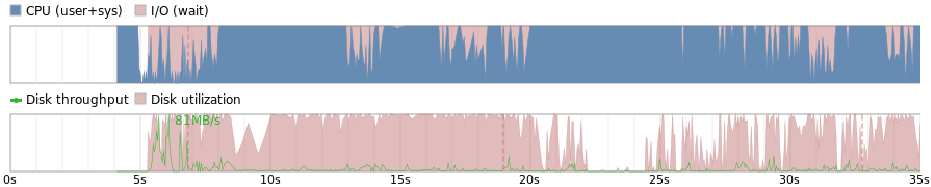
\includegraphics[scale=0.64, trim=1cm 0cm 1cm 0cm]{boot_first35seconds.png}
  \caption[CPU and disk activity for a booting Ubuntu VM in the first 35
  seconds after \texttt{init} is spawned]%
  {CPU and disk activity for a booting Ubuntu VM in the first 35 seconds after \texttt{init} is spawned.
  The first few seconds show no activity because
  the data collection daemon takes a few seconds to start.}
  \label{boot:first35}
\end{figure}

\begin{figure}[h]
  \center
  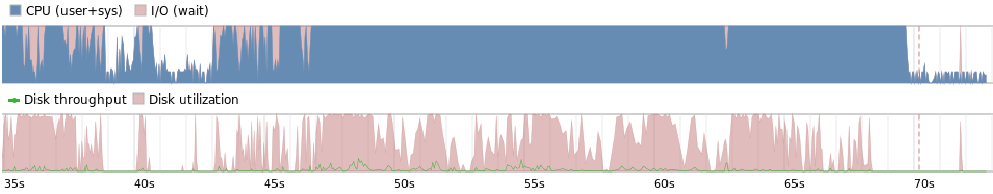
\includegraphics[scale=0.6, trim=1cm 0cm 1cm 0cm]{boot_last35seconds.png}
  \caption[(... continued) CPU and disk activity for a booting VM
  35 seconds after \texttt{init} is spawned. ]%
  {(... continued from Figure \ref{boot:first35}) CPU and disk activity for a booting Ubuntu VM 35 seconds after \texttt{init} is spawned.}
  \label{boot:last35}
\end{figure}

Figures \ref{boot:first35} and \ref{boot:last35}
illustrate the CPU usage and disk activity 
of an Ubuntu 10.10 VM that takes about 70 seconds
to complete the sixth step of the boot process (i.e. spawning 
the \texttt{init} process to set up the user environment).
The Linux kernel version is 2.6.35-27-generic
and the VM is configured with a single core processor
with 512 MB RAM. Generated using
the Bootchart utility \cite{mahkovec2005bootchart},
the figures illustrate that
the booting process involves high memory
and CPU overhead (5-70 seconds); they also 
show a glimpse of the well-known fact that memory and CPU
overhead typically dimishes greatly after the boot
process is completed and the machine is
ready for login (70+ seconds). This disparity
in CPU/memory usage is the source of the boot storm problem;
a single host can handle many VMs in
steady-state usage but gets crippled
when the same VMs boot up concurrently.

In the last step of the booting
process (step 6), \texttt{init} typically
runs many scripts located in 
specific directories such as \texttt{`/etc/rc'}
or \texttt{`/etc/init.d/'}. While the myriad Linux distributions
can have their own variants of \texttt{init} binaries
(e.g. \texttt{SysV}, or \texttt{systemd} or \texttt{Upstart}),
the \texttt{init} process always directly/indirectly launches several 
services and daemons to initialize the user desktop
environment. Figure \ref{boot:services} provides a
summary of the specific actions performed by \texttt{init} 
(through the subprocesses or daemons it launches)
for the same Ubuntu VM used for 
Figures \ref{boot:first35} and \ref{boot:last35}.

\begin{figure}[h]
  \center
  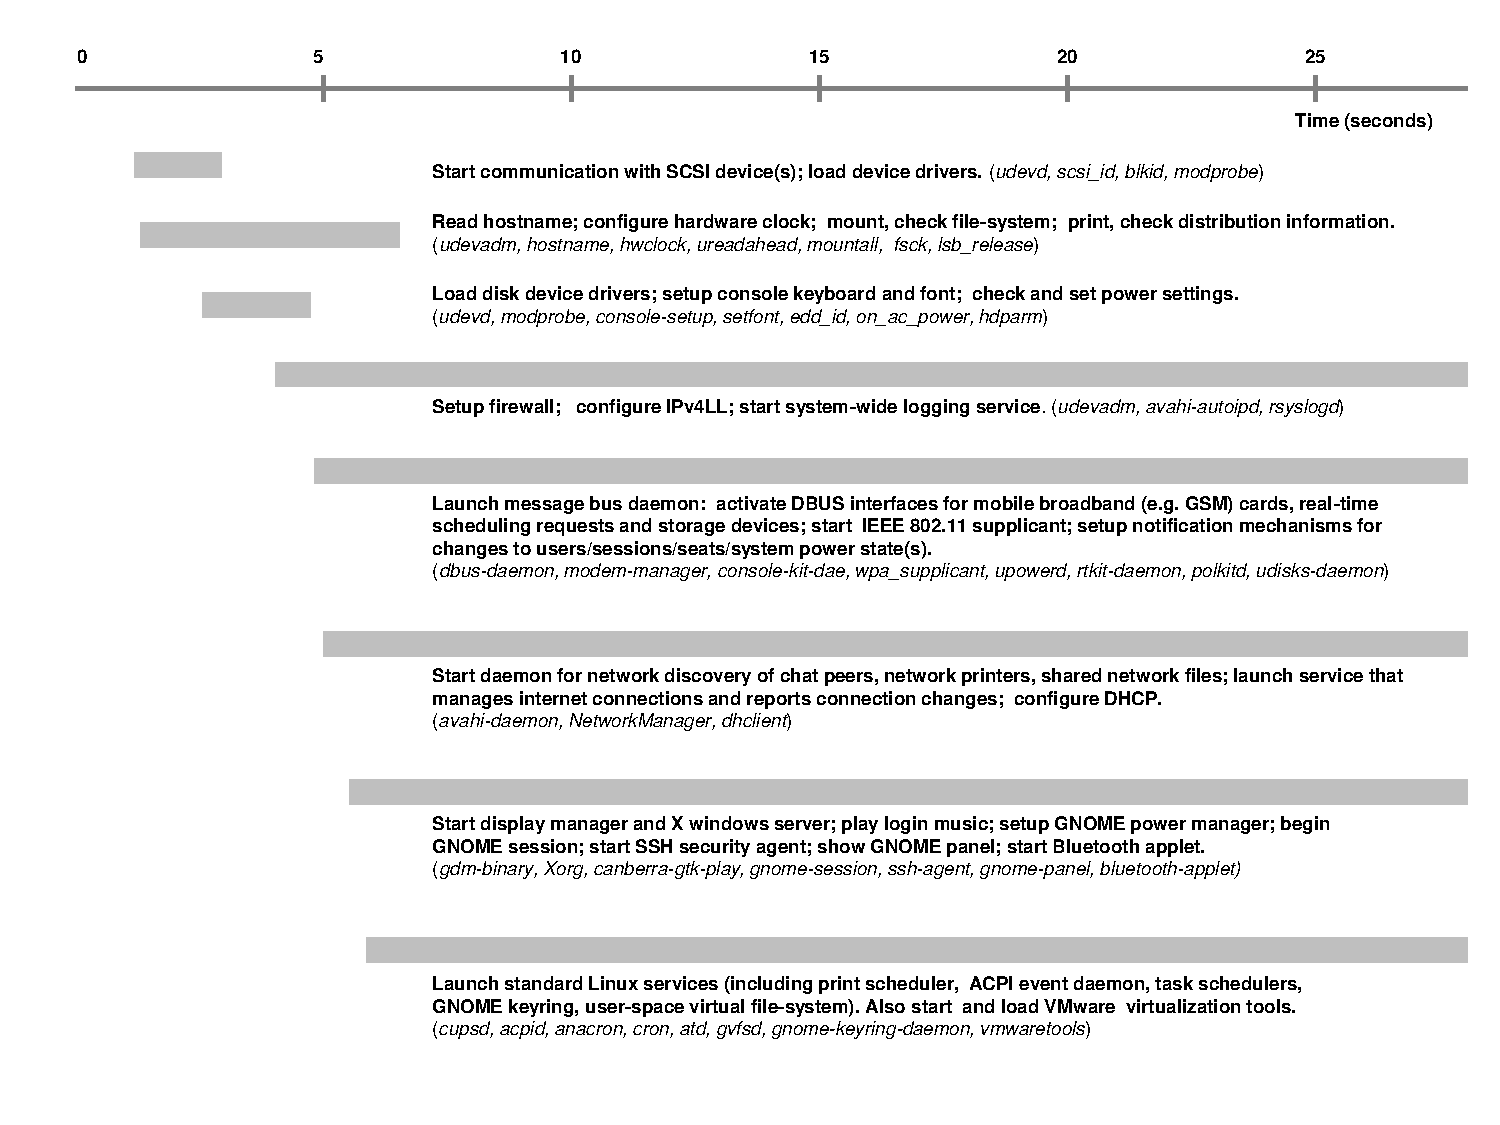
\includegraphics[width=1.0\textwidth, trim=0.5cm 1cm 1cm 1cm]{boottimeline.pdf}
  \caption[A summary of the actions performed by \texttt{init} for a booting VM]%
  {A summary of the actions performed by \texttt{init} for a booting VM;
  this figure has the same timeline (0-70 seconds) as Figures \ref{boot:first35} and 
  \ref{boot:last35}.}
  \label{boot:services}
\end{figure}

In fact, the \texttt{init} process actually launched 361 children processes (directly
and indirectly) over the 70 second period summarized by Figure \ref{boot:services}.
Most of them were ephemeral processes; several processes were repeatedly launched
in different contexts (e.g. \texttt{getty} or \texttt{grep}). The processes singled out
in Figure \ref{boot:services} are the ones that either 
stayed alive through most of the boot process till the end, performed important
boot actions, or spawned many sub-processes themselves.

\section{Data Collection Scheme} \label{datacollection}
\begin{figure}[h]
  \center
  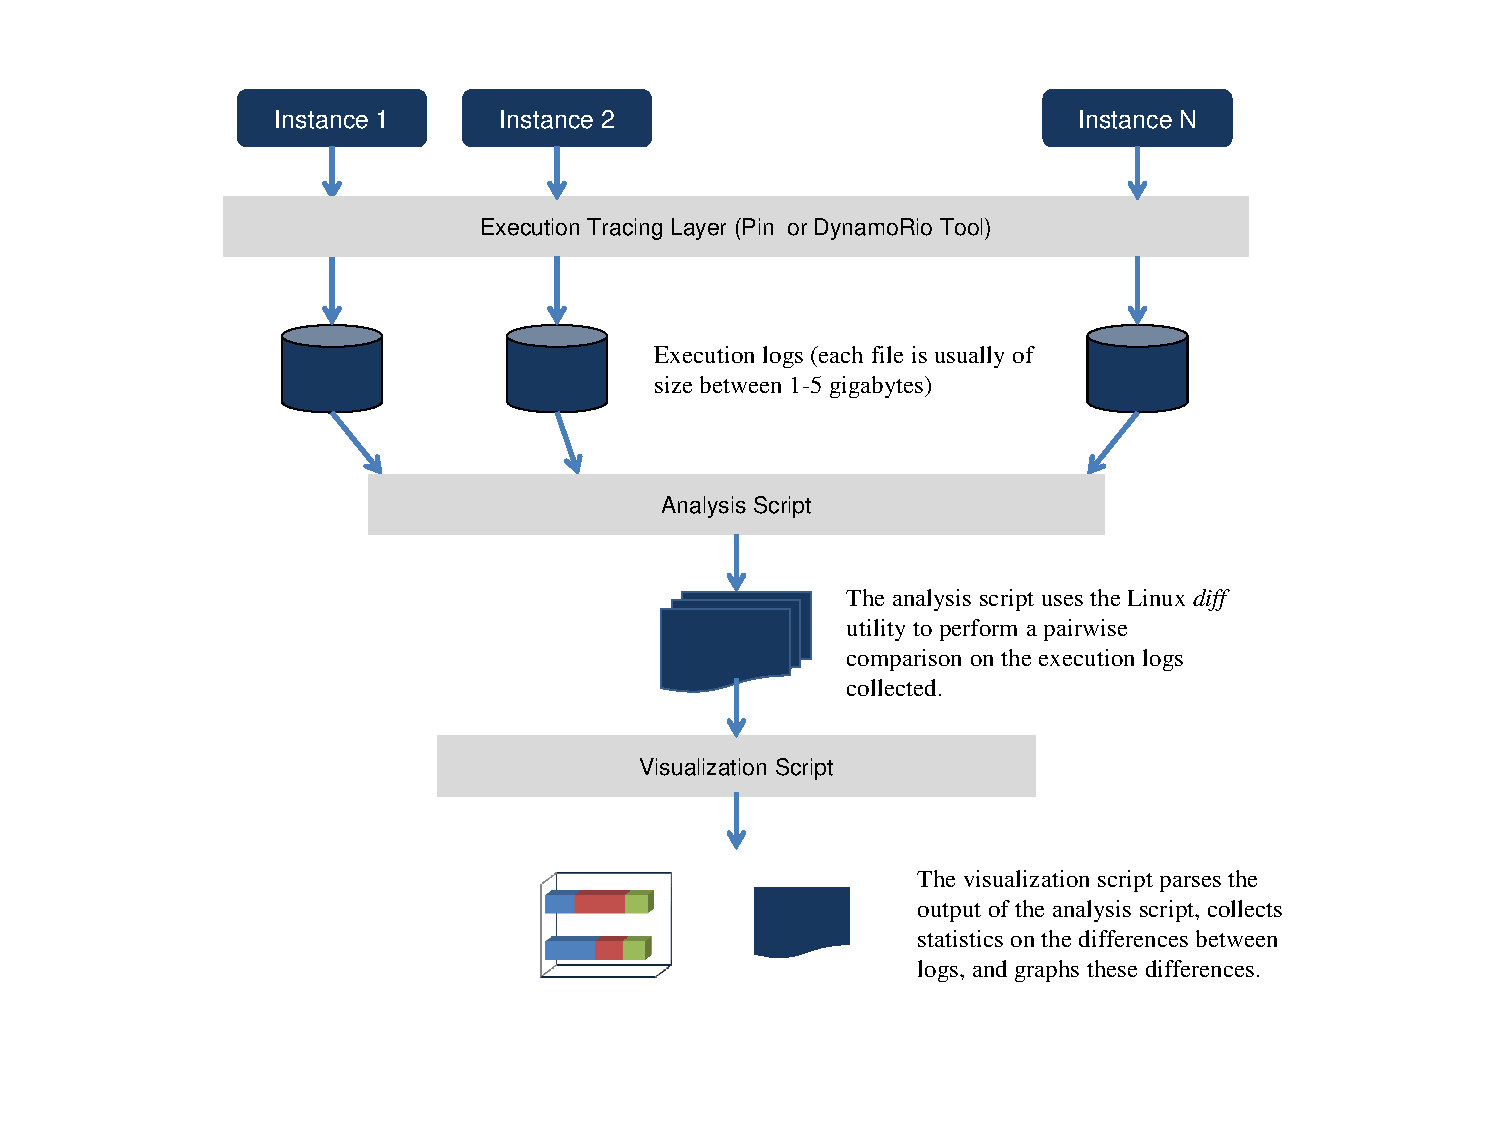
\includegraphics[width=1.0\textwidth, trim=1cm 1cm 1cm 1cm]
                  {naivedatacollection.pdf}
  \caption[Steps involved in measuring execution nondeterminism]%
  {Steps involved in measuring execution nondeterminism.}
  \label{data:naive}
\end{figure}

Pin and DynamoRio are runtime frameworks that enable inspection
and arbitrary transformation of user-mode application code as it executes.
We used both Pin and DynamoRio to study the behavior
of Linux services to verify
the accuracy of our results. However, we relied on Pin more 
than DynamoRio because it gets injected into application code
earlier than DynamoRio and thus provides greater
instruction coverage for our purpose.  Figure \ref{data:naive} shows the simple steps involved
in collecting data on nondeterminism using
dynamic instrumentation. The next section 
explains each of these steps in detail, 
using a simple ``Hello, world!'' program as an example.

\subsection{Measuring nondeterminism in a simple $C$ program} \label{ch:hw}
This section outlines the data collection scheme
described in Figure \ref{data:naive} in detail with the help
of an example:  the simple ``Hello, world!'' program
outlined in Figure \ref{source:hw}.
For this example, we disabled ASLR (Address Space Layout
Randomization) on the Ubuntu VM described in section \ref{linuxboot}. \newline

\begin{figure}[h]
  \lstset{frame=shadowbox, rulesepcolor=\color{Gray},
    basicstyle=\small, numbers=left, numberstyle=\footnotesize}
  \lstinputlisting[language=C]{helloworld.c}
  \caption[A ``Hello, world!'' program in C.]%
          {A ``Hello, world!'' program in C. }
          \label{source:hw}
\end{figure}

\noindent {\bf Execution Tracing Layer} \newline
As shown in Figure \ref{data:naive}, the first step
in data collection involves running the target program
a few times across identical VMs. Ideally, these 
different executions are done concurrently or as
close as possible in time to model the boot storm scenario accurately. 
In our scheme, we wrote a Pin tool that:
\begin{enumerate}
\item logs each x86 instruction executed by 
  the target process, along with the 
  new values of any affected registers, 
\item records values written to or 
  read from memory,
\item intercepts all signals received, and records the instruction counts 
  corresponding to the timing of any signals, and
\item monitors all system calls made by the target process,
  and logs any corresponding side-effects to memory or registers.
\end{enumerate}

Implementation of the execution tracing layer required
a close examination of the Linux system call interface,
because we had to identify the side-effects of each system call. 
Figure \ref{hw:logsys} shows an excerpt from a trace file
generated by our Pin tool while running the ``Hello, World'' 
program. Our tool records and analyzes
every instruction executed in user-space by the process
for the ``Hello, world'' program once Pin gets control; 
this allows us to include program initialization
and library code in our analysis.

\begin{figure}[h]
  \center
  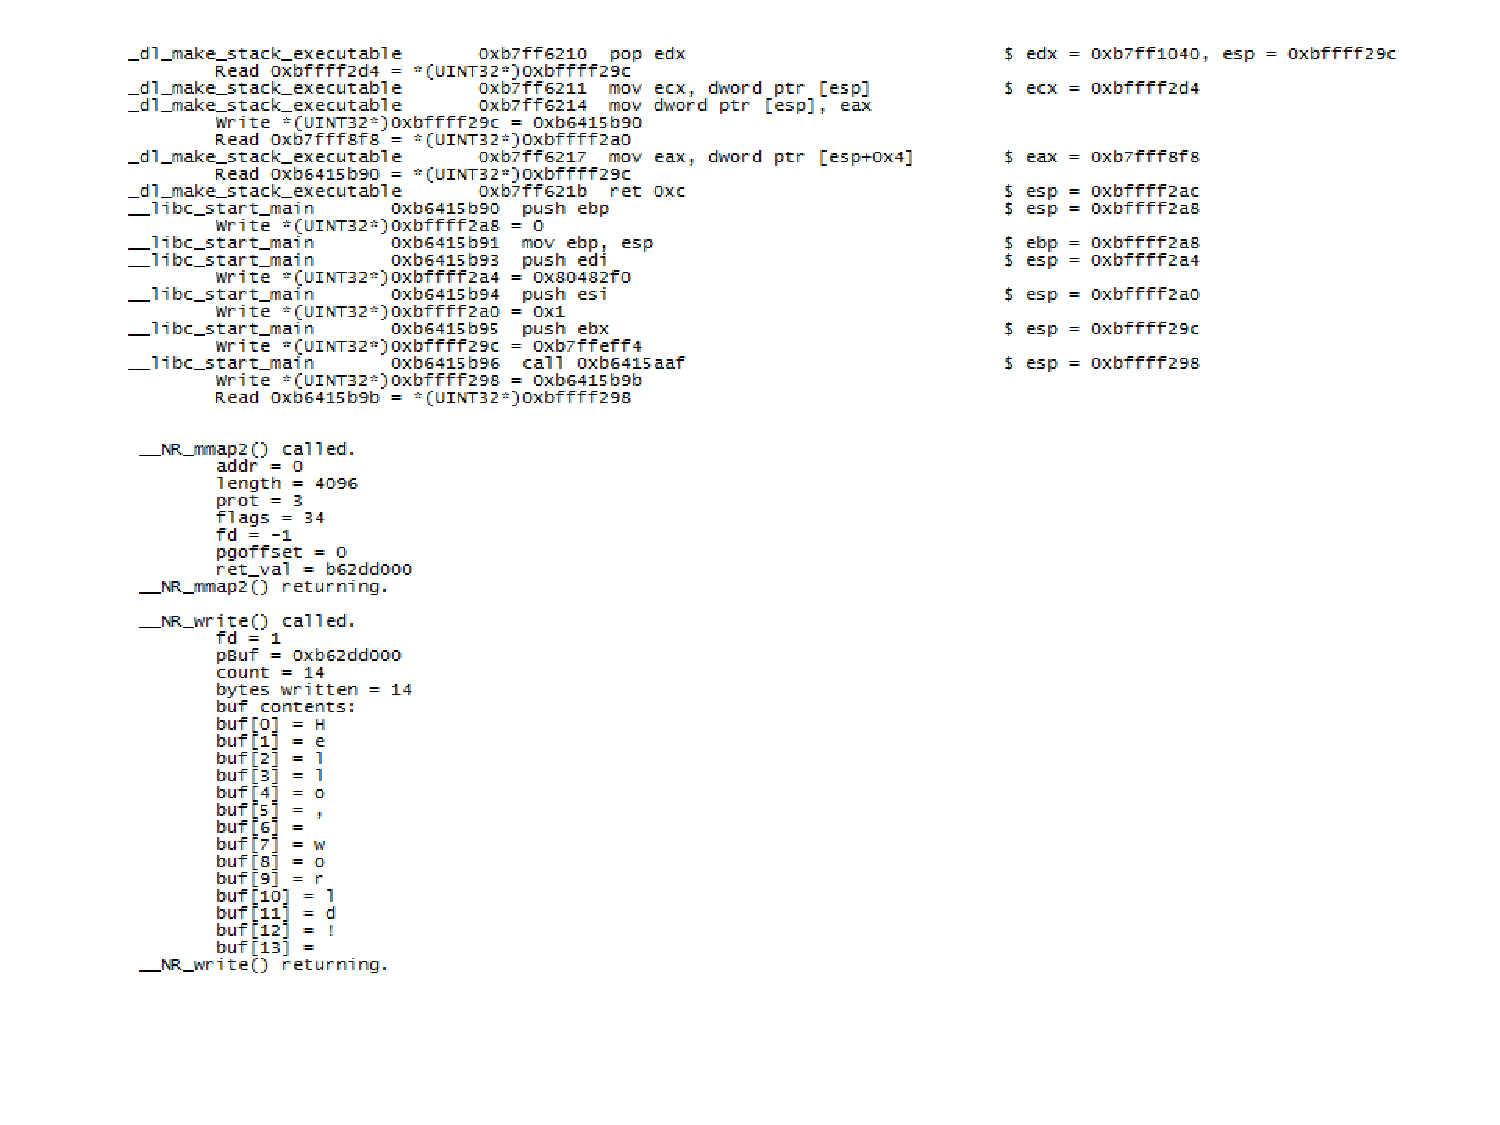
\includegraphics[scale=0.50, trim=2cm 2cm 2cm 0.5cm]{log.pdf}
  \caption[An excerpt from the log files generated by the execution tracing layer]%
          {An excerpt from the log files generated by the execution tracing layer.
          The top half shows some x86 instructions executed 
          in user-space by the ``Hello, world!'' process, including instruction addresses, 
          symbolic information (whenever available), affected register values and memory 
          addresses. The lower half shows an excerpt from the system call log.}
  \label{hw:logsys}
\end{figure}
\newpage
\noindent {\bf Analysis Script} \newline
The analysis script uses the Linux \emph{diff} utility
to perform pairwise comparisons of the log files generated 
by multiple executions of the target application. 
Using the \texttt{suppress-common}, \texttt{side-by-side}
and \texttt{minimal} flags, the analysis script
produces two output files: 
\begin{enumerate}
\item A {\em delta} file
that contains only instructions that were 
either conflicting between the two logs or missing in one log, and
\item A {\em union} file that contains all instructions
executed in the two logs, while distinguishing instructions  
included in the delta file from others.
\end{enumerate}

\begin{figure}[h]
  \center
  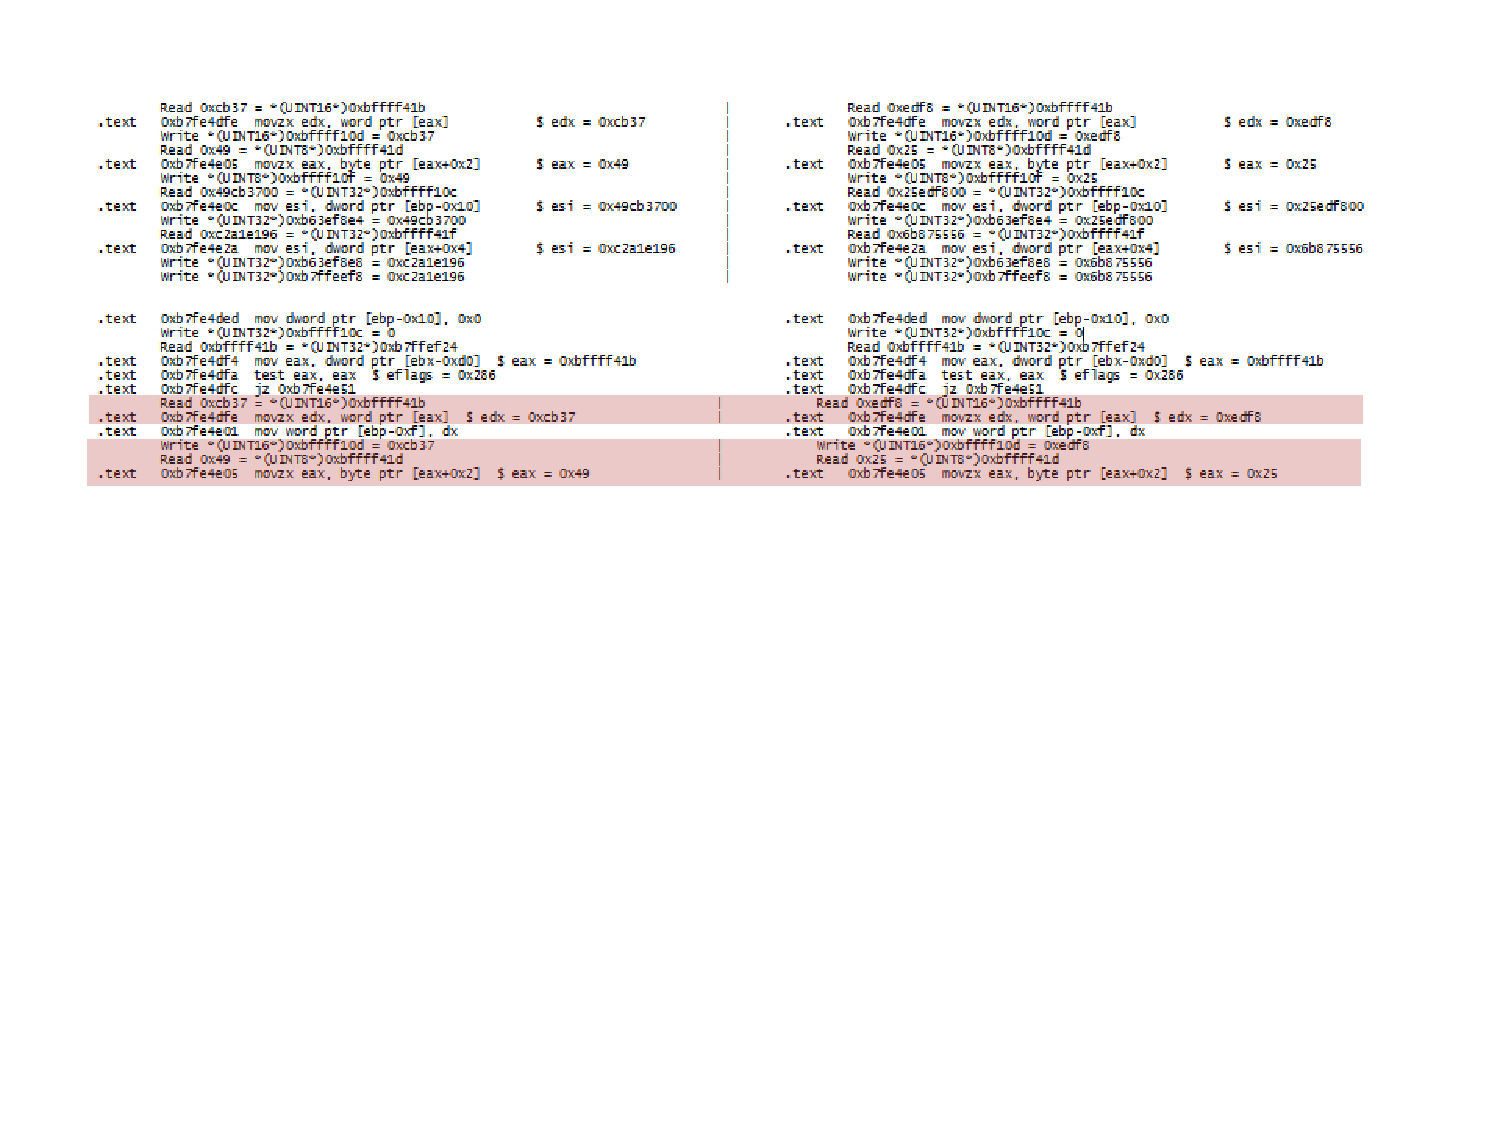
\includegraphics[scale=0.55, trim=2cm 1cm 2cm 1cm]{log2.pdf}
  \caption[Excerpts from the side-by-side diff files generated by the analysis script]%
          {Excerpts from the side-by-side diff files generated by the analysis script.
            The top half shows a few instructions at the start of the delta file;
            all these instructions are different in the two logs (as
            indicated by the $\vert$ in the middle of the line).
            The bottom half shows the corresponding instructions in the union file.
            Conflicting instructions are highlighted with red in the 
            union file (along with the $\vert$ symbol); the other instructions are found in both logs.}
  \label{hw:logsys2}
\end{figure}

Figure \ref{hw:logsys2} shows an excerpt from the 
union and delta files generated for the ``Hello, world!''
program. Given several traces, the delta and union
files can be constructed from the two
executions that are the most or least different, 
or have the median difference. In either case, these generated files can be used to
detect and diagnose sources of nondeterminism
in an application. \newline

\noindent {\bf Visualization Script} \newline
The visualization script reads the union file to 
compute statistics on the extent of differences in the
original logs, and generates diagrams to 
capture the different execution traces of the program.
 
In particular, it derives three key metrics
from the ``union'' file:
\begin{enumerate}
\item {\em Length of Common Prefix {\bf (P):}} This is 
the number of instructions common
to both logs starting from the beginning
and up to the point of first divergence.
\item {\em Longest Common Substring {\bf (LS):}}
This is the largest sequence of adjacent instructions 
that are common to both logs.
\item {\em Longest Common Subsequence {\bf (LCS):}}
Intuitively, this is the ``overlap'' in the logs;
it is the length of the longest sequence of instructions
found in both logs. Instructions in the LCS must be in the same order
in both logs, but they are not required to be adjacent.
\end{enumerate}

For instance, if the first instance of a program
executes the instruction sequence $I_1 = [A, B, C, D, E, F]$,
and the second instance of the same program executes 
the instruction sequence $I_2 = [A, B, X, D, E, F, Y]$,
then: the common prefix is $[A, B]$; the longest
common substring is $[D, E, F]$, and the longest
common subsequence is $[A, B, D, E, F]$. 

In general, the longest common subsequence (LCS) of the two traces is
arguably the most indicative of the extent of determinism
in two executions of a program.
The other two metrics are important 
for evaluating the feasibility of deduplication of execution as
a solution to the boot storm problem. In general,
we want the common prefix (P) and the longest common substring (LS)
of the two logs to be as large as possible to
ensure that concurrently booting VMs do not need to branch
execution or communicate with each other too quickly. This
is further discussed in chapter 5.

For the ``Hello, world!'' program, if ASLR
is enabled, the two logs have very little
overlap ($< 5\%$), and the common
prefix and longest common substring
are on the order of $10$ instructions.
With ASLR disabled, one may 
expect the two traces to look identical (because
of the simplicity of the program), but
there is still some nondeterminism in the 
instruction sequences (see Table \ref{hw:stats}
and Figure \ref{hw:trace}).

\begin{table}
\caption{Nondeterminism profile of ``Hello, world!'' program (ASLR disabled)}
\label{hw:stats}
\begin{center}
\begin{tabular}{||l|c||}\hline
  Common Prefix & 21.49 percent \\\hline
  Longest Common Substring & 67.70 percent \\\hline
  Longest Common Subsequence & 99.98 percent \\\hline
  Conflicts & 0.02 percent \\\hline
  Conflicting Instructions & 32 \\\hline
\end{tabular}
\end{center}
\end{table}

\begin{figure}[h]
  \center
  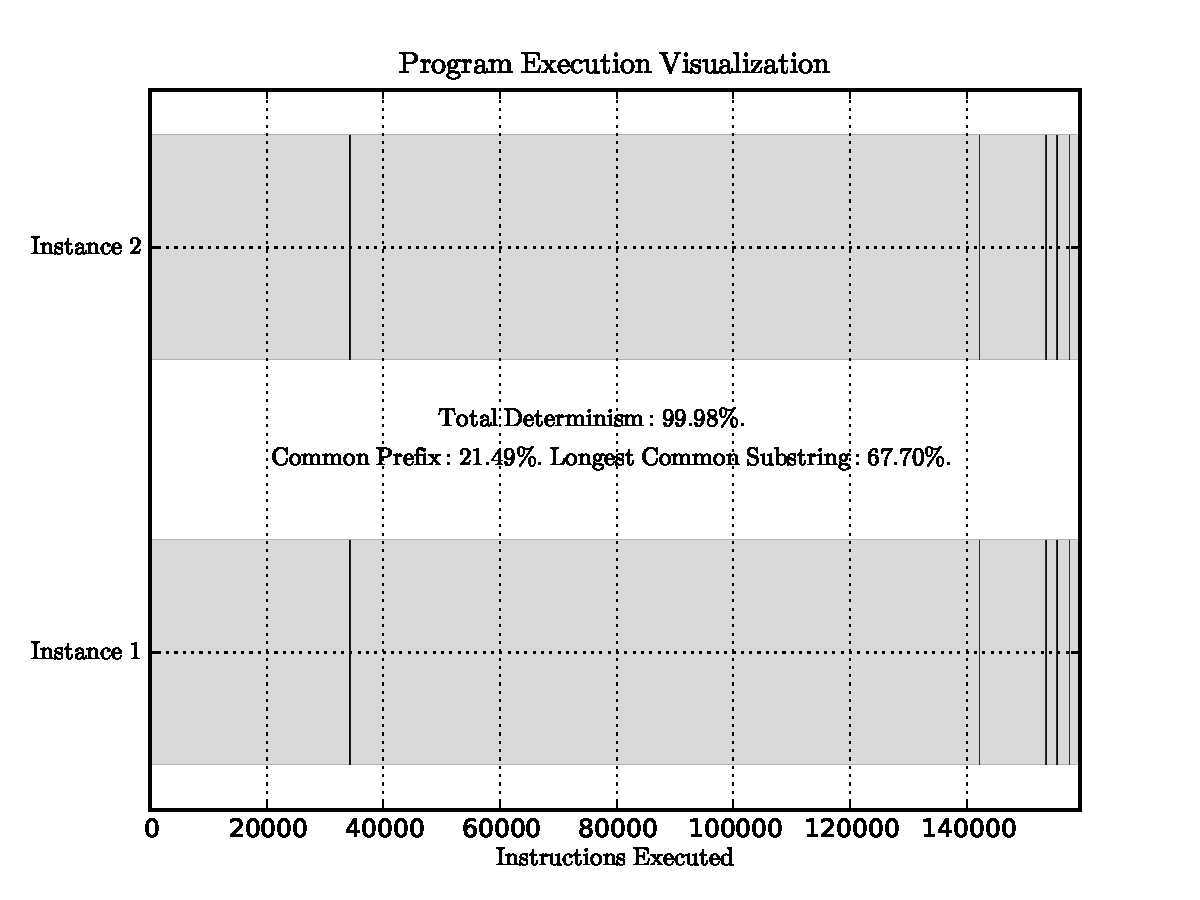
\includegraphics[scale=0.55, trim=0cm 0cm 0cm 0cm]{trace.pdf}
  \caption[Visualization of ``Hello, world!'' program execution]% 
          {Visualization of ``Hello, world!'' program execution.
          The thin black lines represent conflicts between
          the two instances of the program.}
  \label{hw:trace}
\end{figure} 

Figure \ref{hw:trace} shows divergences in program execution
over time. This representation allows
us to visually inspect the union file 
and figure out the distribution and nature of conflicting
instructions. For the ``Hello, world!'' program,
we can see that while divergences were 
spread out near the beginning and end of the program,
they were bursty and short-lived (as indicated
by the thin black lines). This is a common trend, 
even for complex programs such as Linux services,
as discussed in Section \ref{bootresults}.

\subsection{Alternative metrics for measuring nondeterminism} \label{alt:stats}
As mentioned in the previous section, we use the 
common prefix (P), the longest common subsequence (LCS),
the longest substring (LS) and the distribution of
conflicting instructions in separate instruction
streams to measure nondeterminism.

While the conflict ratio measured by our analysis script is usually quite small (e.g. $0.02\%$
for ``Hello, world!''), its importance and impact is disproportionately larger.
As shown in Figure \ref{cascade:ex},  the analysis script 
only considers instructions that originate nondeterminism or actively
propagate it in computing the conflict ratio. 

\begin{figure}[h]
  \center
  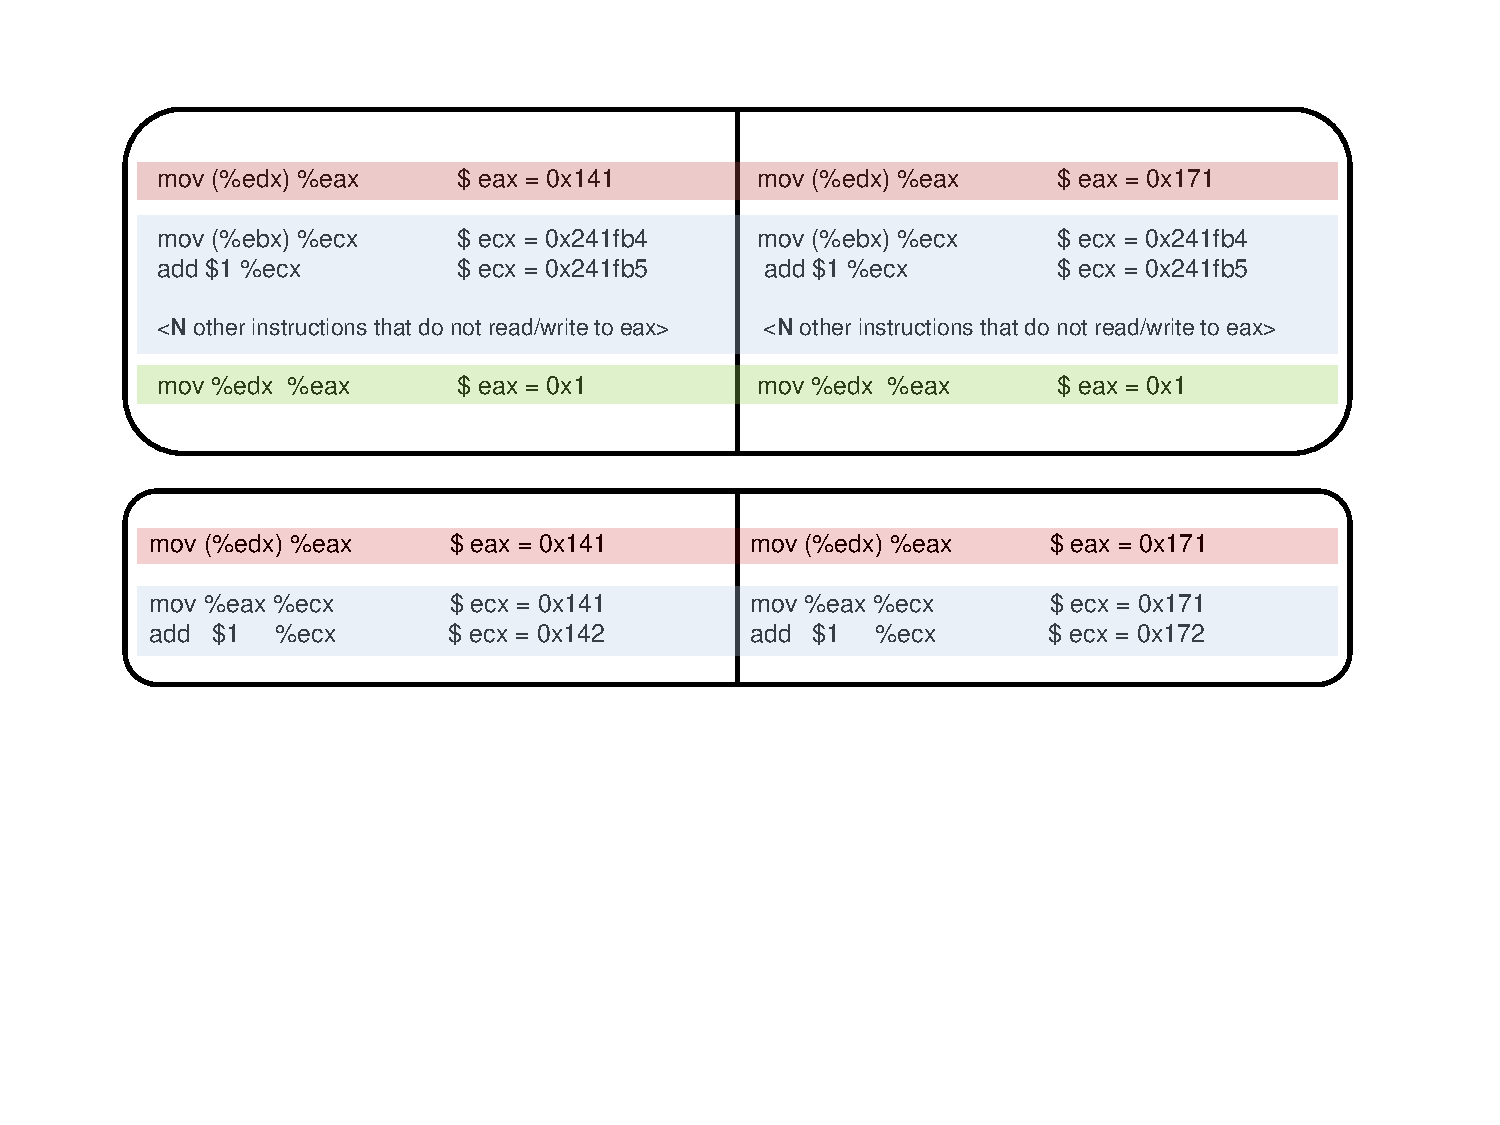
\includegraphics[width=\textwidth, trim=1cm 7cm 1cm 0.4cm]{liveness.pdf}
  \caption[The cascade and propagation effects in measuring nondeterminism.]%
          {The top image shows an example of the cascade effect: the red
          instruction represents a real conflict in \texttt{eax}. The light-blue instructions
          have the same side-effects across the two logs because they don't touch \texttt{eax}.
          The register state only converges after \texttt{eax} is written
          by the green instruction. The cascade effect refers to the nondeterministic register state
          that results in the light-blue instructions because of an earlier conflict, even
          though the instructions themselves are not reading or writing any nondeterministic
          values. If we include the cascade effect, the measured conflict ratio in this
          trace excerpt is $(N+3)/(N+4)$ instead of $1/(N+4)$.  \newline
          
          The bottom image shows an example of the propagation effect: the red instruction again
          represents a conflict in \texttt{eax}. The light-blue instructions do not generate
          any nondeterminism themselves, but they have conflicting side-effects because they
          read \texttt{eax}. In this case, We report a conflict ratio of $1$.}
  \label{cascade:ex}
\end{figure} 

\newpage As shown in Figure \ref{cascade:ex}, the analysis script effectively simulates a taint
analysis on register and memory contents to measure the
true impact of any nondeterminism in a program. 
Grouping instructions that generate and then propagate
nondeterminism makes it easier for us to diagnose the sources of nondeterminism.

% ABSOLUTE TIMING ISSUES

\section{Results for Linux services} \label{bootresults}

\begin{table}[h]
\caption{Nondeterminism profile of Linux services and daemons (ASLR disabled)}
\label{hw:stats}
\begin{center}
\begin{tabular}{||l|c|c|c||}\hline
  Application & Prefix (P) & Longest Substring (LS) &
  Determinism (LCS) \\
  \hline \hline
  \texttt{ntp}, 14 loop iterations & 11.65\% & 22.08\% & 89.21\%
  \\\hline
  \texttt{cron}, 30 loop iterations & 1.58\% & 53.21\% & 98.38\% 
  \\\hline 
  \texttt{cups}, 10 loop iterations & 2.45\% & 25.20\% & 94.25\%
  \\\hline 
  \texttt{daemon A}, $i$ loop iterations & $p$\% & $ls$\% & $lcs$\%
  \\\hline 
  \texttt{daemon B}, $i$ loop iterations & $p$\% & $ls$\% & $lcs$\%
  \\\hline 
  \texttt{daemon C}, $i$ loop iterations & $p$\% & $ls$\% & $lcs$\%
  \\\hline 
  \texttt{daemon D}, $i$ loop iterations & $p$\% & $ls$\% & $lcs$\%
  \\\hline 
  \texttt{daemon E}, $i$ loop iterations & $p$\% & $ls$\% & $lcs$\%
  \\\hline 
  \texttt{daemon F}, $i$ loop iterations & $p$\% & $ls$\% & $lcs$\%
  \\\hline 
  \texttt{daemon G}, $i$ loop iterations & $p$\% & $ls$\% & $lcs$\%
  \\\hline 
  \hline 
  {\bf Aggregate} & {\bf $x$}\% & {\bf $y$}\% & {\bf $z$}\%
  \\\hline 

\end{tabular}
\end{center}
\end{table}

Table \ref{hw:stats} shows the results from applying our data
collection scheme on a set of Linux services and daemons
that are typically launched at boot. We can immediately see that:
\begin{enumerate}

\item The common prefix (P) 
in our sample of Linux services is on average about $3\%$,
which is quite small and indicates that nondeterminism 
typically surfaces relatively early in program execution. 

\item The longest substring (LS), usually close to $25\%$,
is substantially larger than the common prefix (P).
This shows that execution typically does not permanently
diverge in control flow after any initial conflict.

\item The longest common subsequence (LCS) or general determinism
is in general much higher -- about $90\%$ on average -- 
which indicates that a large majority of instructions 
in the Linux services overlap across
different executions. 

\end{enumerate}

Given the discussion in Section \ref{alt:stats}, a conflict ratio
of about $10\%$ on average hints that there is a non-trivial amount of nondeterminism 
in our sample programs, despite a very high average LCS.
The distribution of the $10\%$ conflicting instructions
is surprisingly similar across different programs: 
Figure \ref{ntp:tracech2}, an execution profile of \texttt{ntp}, is representative
of most execution traces. Generally,
conflicting instructions are spread throughout
the program execution, but tend to occur more frequently
towards the end. Nondeterminism does not seem to cause permanent 
execution divergences, even though there is nontrivial amount
of control-flow divergence in some programs. In fact, execution seems to
diverge and reconverge very frequently.

\begin{figure}[h]
  \center
  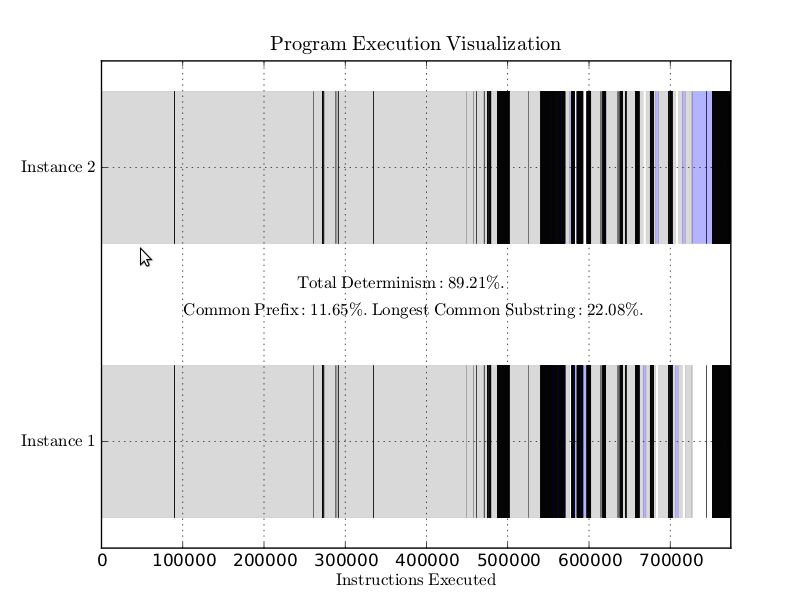
\includegraphics[trim=0cm 0cm 0cm 0cm, scale=0.5]{ntptracech2.jpg}
  \caption[Visualization of \texttt{ntp} program execution]% 
          {Visualization of \texttt{ntp} program execution.
          The thin black lines represent conflicts between
          the two instances of the program, whereas
          the thin blue lines represent control flow
          divergences.}
  \label{ntp:tracech2}
\end{figure} 

The execution profile of \texttt{cron} is somewhat unique
because it has a higher LCS and LS than other traces. It is
difficult to reconcile the low measured conflict ratio for \texttt{cron} (less
than $2\%$), with the higher conflict ratio visually suggested by 
Figure \ref{cron:tracech2}. Figure \ref{cron:zoomtracech2} 
explains this discrepancy: it shows that while
the absolute number of conflicting instructions is small,
these conflicts occur in bursts and visually group together. 

\begin{figure}[h]
  \center
  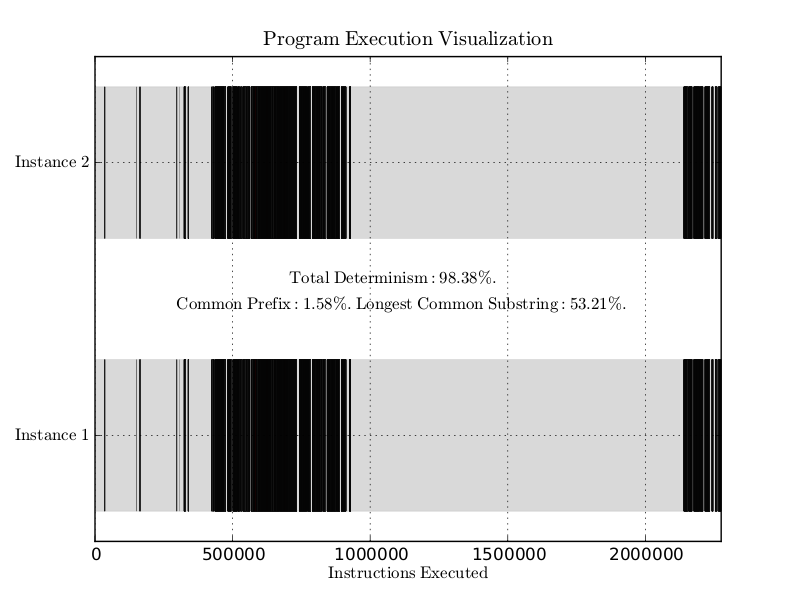
\includegraphics[trim=0cm 0cm 0cm 0cm, scale=0.5]{crontracech2.png}
  \caption[Visualization of \texttt{cron} program execution]% 
          {Visualization of \texttt{cron} program execution.
          The thin black lines represent conflicts between
          the two instances of the program.}
  \label{cron:tracech2}
\end{figure} 


\begin{figure}[h]
  \center
  
\includegraphics[trim=0cm 0cm 0cm 0cm, scale=0.75]{none.jpg}
  \caption[Understanding nature of conflicts in \texttt{cron}]%
  {Looking closely at the \texttt{cron} program execution reveals
    that conflicts occur in bursts.}
  \label{cron:zoomtracech2}
\end{figure} 

While the bursty nature of nondeterminism
is particularly prominent in Figure \ref{cron:zoomtracech2},
it is common to all the services we profiled. Table \ref{burst:stats}
shows that the longest control flow divergence 
or the longest string of consecutive conflicts
is typically very small (i.e. $<<1\%$) 
in our sample programs.

\begin{table}[h]
\caption{Measuring burstiness of nondeterminism in Linux services} 
\label{burst:stats}
\begin{center}
\begin{tabular}{||l|c|c|c||}\hline
  Application & Max. Consecutive Conflicts & Max. Control Flow Divergence \\
  \hline \hline
  \texttt{ntp}, 14 loop iterations & 0.03\% & 2\% 
  \\\hline
  \texttt{cron}, 30 loop iterations & 0.08\% & 0.003\% 
  \\\hline 
  \texttt{cups}, 10 loop iterations & $c$\% & $c$\% 
  \\\hline 
  \texttt{daemon A}, $i$ loop iterations & $p$\% & $ls$\% 
  \\\hline 
  \texttt{daemon B}, $i$ loop iterations & $p$\% & $ls$\% 
  \\\hline 
  \texttt{daemon C}, $i$ loop iterations & $p$\% & $ls$\% 
  \\\hline 
  \texttt{daemon D}, $i$ loop iterations & $p$\% & $ls$\% 
  \\\hline 
  \texttt{daemon E}, $i$ loop iterations & $p$\% & $ls$\% 
  \\\hline 
  \texttt{daemon F}, $i$ loop iterations & $p$\% & $ls$\% 
  \\\hline 
  \texttt{daemon G}, $i$ loop iterations & $p$\% & $ls$\% 
  \\\hline 
  \hline 
  {\bf Aggregate} & {\bf $x$}\% & {\bf $y$}\% %
  \\\hline 
\end{tabular}
\end{center}
\end{table}

\section{Summary}
This chapter presented a brief overview of the Linux boot process,
and demonstrated our methodology for both quantifying and measuring nondeterminism
in programs using dynamic instrumentation. By analyzing user-mode
instructions executed by Linux boot services and daemons, we offered
evidence that Linux services execute highly overlapping instruction
sequences across different runs. We also showed
that any conflicts or nondeterminism in such services occurs in bursts;
nondeterminism does not cause executions to permanently diverge;
divergence and convergence occur very quickly and repeatedly in our
traces.

Chapters 3 and 4 will offer insight into the sources 
of nondeterminism behind these statistics. 
Chapter 5 will look at the implications of our results for a possible
solution to the bootstorm problem.


%% This is an example first chapter.  You should put chapter/appendix that you
%% write into a separate file, and add a line \include{yourfilename} to
%% main.tex, where `yourfilename.tex' is the name of the chapter/appendix file.
%% You can process specific files by typing their names in at the 
%% \files=
%% prompt when you run the file main.tex through LaTeX.
\newenvironment{mylisting}
{\begin{list}{}{\setlength{\leftmargin}{1em}}\item\scriptsize\bfseries}
{\end{list}}

\chapter{Sources of Nondeterminism}
This chapter summarizes the myriad sources of nondeterminism
in Linux services encountered in this work. This
study of nondeterminism reveals
the interactions between user-mode
applications, commonly used system libraries (e.g. the \texttt{libc} library),
the Linux operating system and the external world.
Existing literature on nondeterminism is not 
as comprehensive and does not analyze
Linux system calls in as much detail. 

\section{Linux Security Features} \label{ch3:security}
\subsection{Address Space Layout Randomization (ASLR)}
Address Space Layout Randomization (ASLR) involves random arrangement of
key memory segments of an executing program. When ASLR is enabled,
the virtual addresses for the base executable, shared libraries, 
the heap, and the stack are different every time the program is run.
ASLR hinders several kinds of security attacks in which attackers have to predict
program addresses in order to redirect execution (e.g.
\emph{return-to-libc} attacks). 
As mentioned earlier, As mentioned earlier, two execution traces of a
simple ``Hello, World!" program in $C$ are almost entirely different
when ASLR is enabled. Instruction addresses are different; 
memory addresses (especially stack addresses) are all different as well.

Existing record-and-replay systems sometimes overcome ASLR by
forcing the operating system to use the same address space layout across
different runs. A slightly more complicated approach would involve
using base/offset computations to translate equivalent 
addresses between two different executions. 
We simply disabled ASLR for our experiments using the following command:
\texttt {sudo kernel.randomize\_va\_space=0}.

\subsection{Canary Values and Stack Protection}
Copying a \emph{canary} -- a dynamically chosen global value -- onto the stack below the return
address can help detect buffer overflow attacks, because 
an attack that overwrites the return address will also overwrite
the stack copy of the canary. Before a \texttt{ret}, a simple comparison of the global (and unchanged) canary
value with the (possibly changed) stack copy can prevent a buffer overflow attack.

In 32-bit Linux distributions, the $C$ runtime library, 
\texttt{libc}, provides a canary value in \texttt{gs:0x14}.
If stack smashing protection (SSP) is enabled when a program is compiled,
\texttt{gcc} adds instructions that use the canary value
in \texttt{gs:0x14} to detect buffer overflow attacks.
As Pin gets control of the application before \texttt{libc}
initializes \texttt{gs:0x14}, multiple execution traces of a program
will diverge when \texttt{gs:0x14} is initialized and subsequently
read.  The manner in which the canary value in \texttt{gs:0x14} is initialized
depends on the \texttt{libc} version.
If randomization is disabled, \texttt{libc} will store a fixed terminator canary value (0xff0a0000)
in \texttt{gs:0x14}; this does not lead to any nondeterminism.
However, when randomization is enabled, 
some versions of \texttt{libc} store a random word in \texttt{gs:0x14} by reading from \texttt{`/dev/urandom'}
or by using the \texttt{AT\_RANDOM} bytes provided by the kernel (see Section \ref{ch3:rand}). 

Dynamic instrumentation can be used to force canary values
to agree across distinct executions of the same program:
instructions that initialize \texttt{gs:0x14} can be
modified or replaced, or the \texttt{AT\_RANDOM} bytes provided by the kernel can be
modified before they are read by the application, or reads from \texttt{`/dev/urandom'} can be 
intercepted.

\subsection{Pointer Guard / Encryption}
Many stateless APIs return data-pointers to clients 
that the clients are supposed to simply supply as arguments
to subsequent function calls. 
For instance, the \texttt{setjmp} and \texttt{longjmp} functions
can be used to implement a try-catch block in $C$: \texttt{setjmp} uses 
a caller-provided, platform-specific \texttt{jmp\_buf} structure
to store important register state that \texttt{longjmp} later reads to simulate a return from \texttt{setjmp}.
Since the \texttt{jmp\_buf} instance is transparent to clients of \texttt{setjmp}
and \texttt{longjmp}, it is possible that the clients may advertently or inadvertently
overwrite the return address stored in it and cause
\texttt{longjmp} to fail.

Many APIs use simple encryption schemes to detect mangled data structures.
For instance, in 32-bit Linux, \texttt{libc} provides
a {\em pointer guard}  in \texttt{gs:0x18}. This pointer guard has a different value
across multiple runs of a program, just like the \texttt{libc} canary value.
The idea behind the pointer guard is the following: to encrypt a sensitive address $p$, a program
can compute $s = p$  $\oplus  $ \texttt{gs:0x18}, optionally add some bit rotations, and store it in a structure
that gets passed around. Decryption can simply invert any bit rotations, 
and then compute $p = s$ $\oplus  $ \texttt{gs:0x18} back. Any blunt writes to the structure from clients will be detected because 
decryption will likely not produce a valid pointer. 
Pointer encryption is a useful security feature for some APIs
and is used by some versions of \texttt{libc} to protect addresses stored in \texttt{jmp\_buf}
structures.

Initialization of the \texttt{libc} pointer guard can therefore be a source of nondeterminism
program execution. In some versions of \texttt{libc}, the value of \texttt{gs:0x18} is the same
as the value of \texttt{gs:0x14} (the canary). In others,
the value of \texttt{gs:0x14} is \texttt{XOR}ed with 
a random word (e.g. the return value of \texttt{rdtsc} x86 instruction,
or some \texttt{AT\_RANDOM} bytes provided by the kernel) to compute
the pointer guard. In any case, the value of the pointer
guard can be made to agree across different instances
of the same program via dynamic instrumentation: 
the instructions that initialize \texttt{gs:0x18} can
be modified or replaced, or the \texttt{rdtsc} instruction
can be intercepted and emulated, or the  \texttt{AT\_RANDOM} bytes provided by the kernel can be
replaced before they are ever read.

\section{Randomization Schemes} \label{ch3:rand}
As already clear from Section \ref{ch3:security}, 
randomization schemes constitute a major source of nondeterminism 
in programs.
Applications generally use pseudorandom number generators (PRNGs)
for randomization; they rely on the {\em seeds} to the PRNGs
to be different across multiple program executions 
to generate truly random values. PRNG seeds are typically 
computed from several external sources:

\begin{itemize}

\item {\em The} \texttt{`/dev/urandom'}{\em special file}: Linux allows
running processes to access a random number generator through this special file. The entropy generated
from environmental noise (including device drivers)
is used in some implementations for the kernel random number generator.
\item \texttt{AT\_RANDOM} {\em bytes}: 
Making system calls to open, read and close the
\texttt{`/dev/urandom'} file only for a
few random bytes can be computationally expensive. So 
some recent versions of the Linux kernel supply
a few random bytes to all executing programs
through the \texttt{AT\_RANDOM} auxiliary vector.
ELF auxiliary vectors are pushed on the program
stack below command-line arguments and environmental
variables before the program starts executing.

\item {\em The} \texttt{rdtsc} {\em instruction}:
The \texttt{rdtsc} instruction provides an approximate number of ticks since
the computer was last reset, which is stored in a 64-bit register present
on x86 processors. Computing the difference between two successive
calls to \texttt{rdtsc} can be used for timing, whereas a single
value returned \texttt{rdtsc} lacks any useful context.  
The instruction has low-overhead, which makes it suitable for generating a random value
instead of reading from \texttt{`/dev/urandom'}. 

\item {\em The current time or process ID}: Many applications simply make a system call
to get the current time or the process ID, and use the returned value to seed their PRNGs. 

\item {\em Miscellaneous}: There
are several creative ways to seed random number
generators (e.g. {\em www.random.org}),
but thankfully we have not observed them
in the Linux services we have analyzed.
      
\end{itemize}

To overcome nondeterminism resulting from randomization, 
we need to intercept the standard techniques
used by programs to seed PRNGs.
Dynamic instrumentation can be used to 
intercept reads from \texttt{`/dev/urandom'}
and emulate \texttt{rdtsc} instructions.
Nondeterminism from process IDs
can be controlled by virtualizing the process ID
layer (Section \ref{ch3:pid}), and nondeterminism
from time can be controlled by intercepting
time-related system calls and forcing
agreement between concurrently executing 
instances (Section \ref{ch3:time}).

\section{Process Identification Layer} \label{ch3:pid}
% pid, signal(pid), /proc/ filesystem layer

In the absence of a deterministic operating system layer, process IDs assigned
to Linux services at boot-time are not predictable.
For instance, a nondeterministic scheduler 
could lead to several possible process creation sequences.

Given the unpredictability of process IDs,
Linux system calls that directly or indirectly
interact with the process identification layer can cause divergences
in distinct executions of the same program.
For instance, system calls that return a process ID e.g.
\texttt{getpid} (get process ID), \texttt{getppid} (get
parent process ID), \texttt{fork/clone} (create a child process),
\texttt{wait} (wait for a child process to terminate)
can return different values across executions. System calls that take process IDs 
directly as arguments such as \texttt{kill} (send a signal to a specific
process), \texttt{waitpid} (wait for a specific child process to terminate)
can similarly propagate any nondeterminism.
In fact, \texttt{libc} stores a copy of the current process ID in \texttt{gs:0x48},
so reads or writes to this address can cause conflicts.

There are certain obscure interactions
between the Linux kernel and executing programs
where process IDs also show up. For instance:
\begin{itemize} 
\item If a process registers a signal handler with the \texttt{SA\_SIGINFO}
bit set, then the second argument passed
to the signal handler when a signal occurs is of type \texttt{siginfo\_t*}.
The member \texttt{siginfo\_t.si\_pid} will
be set if another process sent the signal 
to the original process. 
\item The Linux kernel will sometimes use process IDs 
to indicate the intended recipients of its messages. 
For instance, \texttt{Netlink} is a socket-like
mechanism for inter process communications (IPC)
between the kernel and user-space processes.
\texttt{Netlink} can be used to pass
networking information between kernel
and user space, and some of its APIs 
use process IDs to identify communication
end-points. \end{itemize}

Instead of exhaustively searching the entire
Linux system-call interface, we found these obscure sources of
nondeterminism by incrementally adding logic 
for system calls actually used during execution
to our Pin tracer tool (Section \ref{ch:hw}) .

Process IDs can be used to seed a PRNG (Section \ref{ch3:rand}),
or access the \texttt{`/proc/[pid]'} directory (Section \ref{ch3:procfs}). 

\begin{figure}[h]
  \center
  
\includegraphics[trim=0cm 0cm 0cm 0cm, scale=0.75]{none.jpg}
  \caption[Virtualizing the process ID layer using Pin]% 
  {We intercept all system calls and communications
  between the Linux user and kernel space; we
  translate between real and virtual process IDs
  to trick the kernel and the user-space programs.}
  \label{ch3:pidfig}
\end{figure} 

Figure \ref{ch3:pidfig} shows how we can use dynamic instrumentation
techniques to virtualize and determinize the process ID layer in Linux.
Using these techniques, we were able to avoid modifying
the Linux operating system and existing programs
altogether.

\section{Time} \label{ch3:time}
Concurrent runs of the same program will typically
execute the same instructions at (slightly) different times.
Thus, any timestamps read or written
by programs are clearly a significant source of nondeterminism.

Any Linux system calls that directly or indirectly return timestamps
can cause nondeterminism. For instance:

\begin{itemize}
\item The \texttt{time}, \texttt{gettimeofday} and \texttt{clock\_gettime}
 system calls return the current time.
\item The \texttt{times} or \texttt{getrusage} system calls
return process/CPU time statistics.
\item The \texttt{adjtimex} system call is used 
by clock synchronization programs (e.g. \texttt{ntp}) 
and can returns a kernel timestamp indirectly via 
a \texttt{timex} structure.
\item Programs can access the hardware clock
through \texttt{`/dev/rtc'} and can
read different values for the current time through the \texttt{RTC\_RD\_TIME} \texttt{ioctl}
operation.
\item Many system calls that specify a timeout
for some action (e.g. \texttt{select}, \texttt{sleep} or \texttt{alarm})
inform the caller of any unused time from the timeout interval if they
return prematurely.
\item The \texttt{stat} family of system calls returns file
   modification timestamps;
   application files typically contain timestamps;
   network protocols use timestamps frequently as well.
   (See Section \ref{ch3:filenetio}
\end{itemize}

To overcome nondeterminism from time-related system calls,
we can use dynamic instrumentation to force agreement between 
any timestamps returned across concurrent
executions (taking care to preserve monotonicity).
This creates the illusion that multiple executions
are occuring precisely at the same time. When timestamps
returned from system calls are only compared, they
can be replaced with deterministic ordinal values that 
perserve the comparison (e.g 0 or 1). 

\section{External I/O} \label{ch3:filenetio}
\subsection{File I/O} \label{ch3:fileio}
If two executions of the same program read different
file contents (e.g. cache files), then
there will naturally be some execution divergence.
However, for concurrently executing Linux services,
differences in file contents typically arise
from process IDs (Section \ref{ch3:pid}) or timestamps (Section \ref{ch3:time})
rather than semantic differences.
If those factors are controlled, file contents rarely differ.

Apart from minor differences in file contents,
nondeterminism can arise from different file 
modification (\texttt{mtime}), access (\texttt{atime}) or status-change (\texttt{ctime})
timestamps.
The \texttt{stat} system call is usually made for almost
every file opened by a program; the timestamps
in the buffer written by the system call invariably
conflict between executions. Most of the time,
these timestamps are not read by programs,
so there is little propagation. On occasion, 
however, a program will use these timestamps
to determine which file out of a group is the most recent, 
or whether a file has been updated
and needs to be refreshed. Usually, simply
replacing the time values with fixed ordinal values
that preserve the ordering of timestamps is sufficient
to control such nondeterminism.

When a program wishes to open
a file in append-mode, it uses \texttt{lseek}
with \texttt{SEEK\_END} to move
the file cursor to the end,
before any \texttt{write}s take place.
The return value of \texttt{lseek} is the
updated cursor byte offset into the file.
Clearly, if the length of a file is different across
multiple exections of a program, then
\texttt{lseek} will return conflicting values.
Many Linux services maintain log files
which can have different lengths due
to conflicts in an earlier execution; \texttt{lseek}
further propagates them. To overcome
such nondeterminism, older log files
must be identical at the beginning 
of program execution.

Ultimately, if two input files are semantically different between
different executions of a program, then 
execution will inevitably diverge. However,
the approaches mentioned in this chapter
are typically sufficient to ensure that
file contents rarely differ in Linux services,
if at all.

\subsection{Network I/O} \label{ch3:netio}
The \texttt{libc} network initialization
code loads several configuration files
into memory (e.g. \texttt{`/etc/resolv.conf'}). 
The \texttt{dhclient} daemon updates \texttt{`/etc/resolv.conf'} 
with information from the DHCP server periodically in the background.
Differences in
the content, timestamps or lengths
of such configuration files can cause nondeterminism.
In fact, calls to \texttt{getaddrinfo} 
periodically \texttt{stat} configuration files (e.g. \texttt{`/etc/gai.conf'})
to see if they have been changed in the background since they were last read. 
In our experiments, only the file timestamps of these configuration files vary
between different executions, so the strategies described in Section \ref{ch3:fileio} 
are sufficient to ensure deterministic execution. 

IP addresses are resolved identically by concurrently executing programs 
in our experiments; however, if DNS-based
load-balancing schemes are used, this may not be the case.
In these rare cases, dynamic instrumentation can be used
to enforce agreement between different executions.

If the contents read from sockets
vary across different executions, dynamic instrumentation can be used to 
intercept Linux socket calls
and modify their side-effects to be identical. If
many concurrent executions are reading data from the
same network source, this simply simulates the possibility that all instances
see the same results as the first instance. 
While these semantics are sufficient for most Linux services,
we have not needed to use them: in our experiments,
we have only observed nondeterminism
in reads from \texttt{Netlink} sockets.
As mentioned in Section \ref{ch3:pid},
\texttt{Netlink} sockets provide a 
mechanism for inter process communications (IPC)
between the kernel and user-space processes.
\texttt{Netlink} can be used to pass
networking information between kernel
and user space. Netlink sockets
use process IDs to identify
communication endpoints, which can
be different between executions.
Furthermore, a netlink 
socket of the \texttt{NETLINK\_ROUTE}
family receives routing and link updates
from the kernel. \texttt{libc} uses \texttt{RTM\_NEWLINK}
messages to discover the link interfaces 
in the computer. When a new interface
is discovered or reported, the kernel also supplies
interface statistics to \texttt{libc},
such as packets/bytes sent, dropped or
received. These will obviously be different
across different executions. However,
we can easily use dynamic instrumentation
to intercept \texttt{Netlink} communications
and force these statistics to be
identical.

A TCP/IPv4 connection consists of two endpoints,
and each endpoint consists of an IP address and a port
number. Therefore, when a client connects to a server,
an established connection can be thought of as the
4-tuple (server IP, server port, client IP, client port).
Usually three of these four are readily known:
a clients uses its own IP and the
server IP and server port are required. What is not
immediately evident is that the client
side of the connection uses a port number.
Unless a client program explicitly
requests a specific port number,
the port number used is an ephemeral port number.
Ephemeral ports are temporary ports
assigned by the machine's IP stack, 
and are assigned from a dedicated range of
ports for this purpose. When a connection
terminates, an ephemeral port can be recycled.
Since the underlying operating system
is not deterministic, ephemeral
port numbers used by Linux services
tend be different across multiple 
runs. We mask this nondeterminism 
using dynamic instrumentation by
changing the \texttt{bind} or \texttt{connect} 
system call arguments to explicitly request ports
in the ephemeral range rather than letting the kernel 
assign them; alternatively,
we can also virtualize ephemeral ports
similar to how we virtualize process IDs.

\subsection{I/O Polling Engines}


\section{Signals}
% timing e.g. alrms

\section{Inter-thread Communication/Scheduling} 
%scheduler; concurrency

\section{Misc System Calls}
% all statistics

\section{The `/proc/' filesystem}\label{ch3:procfs}








\section{Issues at Stake}
% security: canary aslr etc
% performance & correctness: randomization, ntp (time skew), time monotonic,
% IO aggregation. (acquire lock). 
\section {Summary}

\chapter{{\em Silhouette} Execution} \label{ch:sil}
In the previous two chapters,
we identified how and why
multiple executions of the same
Linux service can diverge in behavior.
In light of our results, this chapter introduces a 
novel design strategy that aims to mitigate the boot storm problem:
{\em silhouette} execution (Section \ref{def:sil}).
For the sake of evaluation, this chapter
presents some design sketches for silhouette
execution for user-mode programs (Section \ref{subsil}).
It also describes the simple simulation techniques we used 
to model the effectiveness of silhouette
execution using our design sketches
(Section \ref{silsimulation}).
From the results of our simulations, we present strategies
to improve the effectiveness of
silhouette execution (Section \ref{silimprove})
and evaluate them (Section \ref{sileval}).
Our simulations show that the proposed designs can be successful
in mitigating the boot storm problem. 

\section{What is {\em Silhouette} execution?} \label{def:sil}
The previous few chapters showed that
distinct executions of the same Linux service
generally execute the same number of instructions
across identical VMs when they start up. If the number of booting VMs for
the same physical host is large (as is 
the case in VDI deployments),
then executing many instructions over
and over again during boot represents a waste of scarce CPU cycles.
{\em Silhouette} execution, in essence, targets
redundant execution of the same instructions across distinct but
identical virtual machines in order to reduce CPU pressure in boot storm
scenarios. 

\newpage
\begin{figure} []
  \centering
  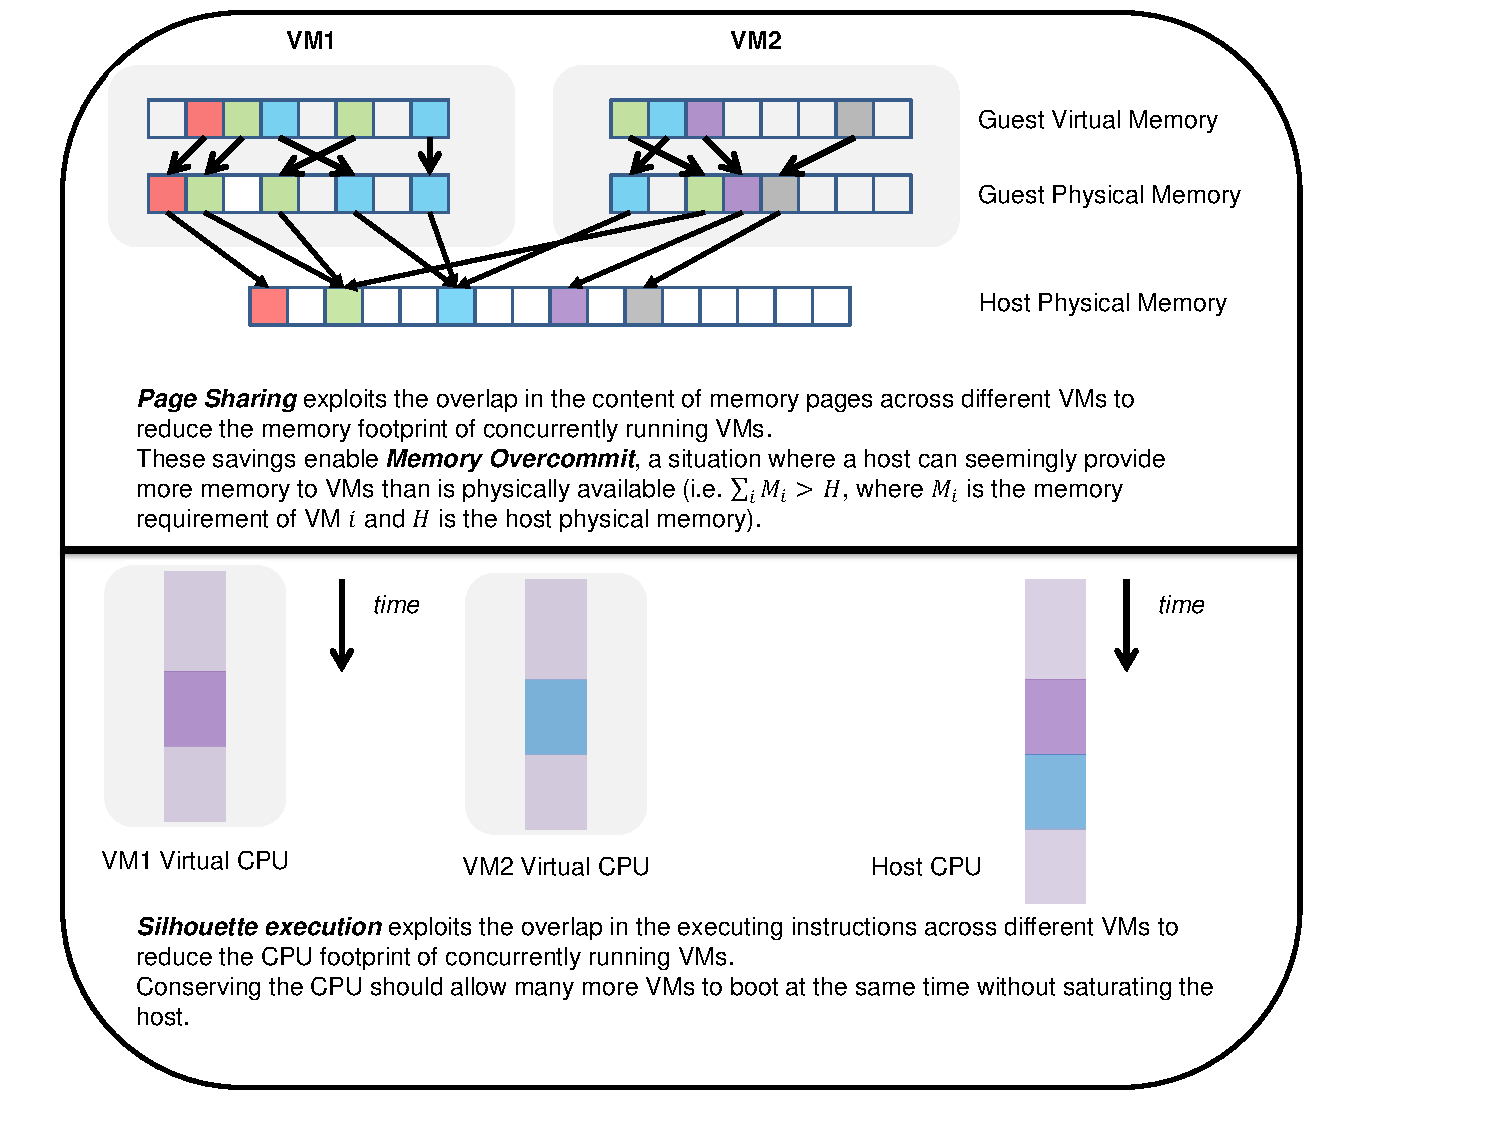
\includegraphics[scale=0.8, trim=2cm 0cm -5cm 0cm]{overcommit.pdf}
  \caption[Silhouette execution is analogous to Page Sharing.]%
          {Silhouette execution is analogous to Page Sharing.}

  \label{silconcept}
\end{figure}

As shown in Figure \ref{silconcept},
silhouette execution is analogous
to page sharing:
both design ideas aim to use hardware
resources effectively to improve VM density per host
in virtualization scenarios.
While page sharing reduces
pressure on the memory subsystem
by identifying and refactoring
overlapping memory contents,
silhouette execution identifies
overlapping instruction streams
and refactors execution to
reduce pressure on the CPU.
Like memory overcommit,
the ultimate aim is to allow a host 
to support VMs that together require
more hardware resources than are really available
in the host.

To the best of our knowledge, silhouette execution is a novel
design idea that has not been
suggested or implemented before.
To study whether this approach
can be effective in reducing CPU pressure
in concurrently booting VMs,
we present some design sketches for implementing silhouette
execution for Linux services in the rest of this chapter. Admittedly,
user-mode instruction streams 
from Linux services capture
a subset of instructions
executed by a booting VM.
However, we focus on 
Linux services as a first step in
studying the feasibility of 
silhouette execution.
After all, as outlined
Section \ref{linuxboot}, booting VMs
can saturate host CPUs when they launch many
identical user-space processes.
For a complete solution, proposed design sketches need to be 
generalized to the execution of entire
VMs themselves; this would require us to precisely
identify the execution differences that can
arise from all software layers inside a VM. \newline

\section{Silhouette Execution for Linux Services} \label{subsil}
For user-mode Linux services, our
proposed design skeletons for silhouette execution
use  information recorded from one
executing program -- the {\em leader} -- to
bypass execution steps of subsequent instances
of the program  -- the {\em silhouettes}. 
Ideally, the leader executes all instructions from the program, 
while the silhouettes execute a much smaller subset
of these instructions.  

\newpage
To maintain correctness in user-space,
silhouettes need only execute: 

\begin{itemize}
\item instructions that can potentially cause the leader's
  execution to differ from the silhouettes (e.g. the \texttt{rdtsc}
  instruction); 
\item instructions that propagate any earlier differences in execution; 
\item instructions that write to memory;
\item system calls that have side-effects to entities
  outside a user-space program
  (e.g. the \texttt{read} system call mutates hidden operating system 
  state associated with file descriptors).
\end{itemize}

If there are no differences between the leader's
execution and a silhouette's, then the silhouette would only
execute the system calls and store instructions
executed by the leader until the login screen is shown.
Executing all the memory writes from the leader
in the silhouettes ensures that the address space and memory
contents of the two instances
evolves in an identical manner. Executing all the system
calls with the same arguments also ensures
that the silhouette's execution is {\em faithful}
to its semantics, that is, the side-effects to the underlying
operating system are maintained till the end.
After we restore the register contents, a silhouette can simply continue
execution independently of the leader.
When the number of system calls and memory writes
is a small fraction of the leader's execution,
this approach can theoretically reduce the stress
placed on the host CPU. 

More generally, when there are instructions
with conflicting side-effects in the leader
and a silhouette, then these instructions
need to be executed by each silhouette independently.
This ensures that the silhouette's execution
semantics are retained. 
It is not known {\em a priori} which instructions in the
two instances of the same program will behave
differently or not.
Our detailed analysis of the various interfaces
between application programs and the operating system
allows us to identify such potential sources of
execution divergence via dynamic 
program inspection.

\newpage
Note that silhouette execution for user-space programs is fundamentally different
from record-and-replay approaches because it
does not semantically alter subsequent executions
of a program by emulating the leader's execution. 
In fact, silhouettes are independent executions of a program
that can potentially branch from the leader's execution at any point.

The next few subsections outline a few
design sketches for implementing silhouette execution
on individual user-space programs
such as Linux services.
We have not implemented these designs.
Instead, we present them here 
to evaluate the effectiveness of silhouette
execution in user-space.

\subsection{{\em Precise Silhouetting}}\label{precise:sil}
Here is a simple design that uses silhouette execution 
to refactor execution in a user-mode program:

\begin{enumerate}

\item We run one program instance -- the {\em leader} -- 
slightly ahead of all other program instances -- the {\em silhouettes}.

\item Using dynamic inspection techniques on the leader, we
\begin{itemize}
\item precisely identify instructions where other instances of the
program could {\em potentially} diverge. We call these instructions {\em fork-points}.
\item collect an {\em execution signature} that summarizes the 
leader's execution between successive fork-points. For a user-space program, 
this includes a record of memory operations and 
deterministic system calls.
\end{itemize}

\item When a leader reaches a fork-point, it sends its
own execution signature from the previous fork-point (or the
beginning of the program) till the current fork-point to all
other silhouettes. 

\item The silhouettes do not execute
all the instructions that the leader executes.
In fact, each silhouette bypasses execution between
two fork-points by executing only the memory
operations and system calls from the 
execution signature sent by the leader,
and restoring the register state at the end.

\item 
When a silhouette reaches a fork-point, it 
independently executes the {\em forking} instruction
and observes its side-effects.
The forking instruction may or 
may not behave differently
in a silhouette than the leader.

\begin{itemize}
\item If the forking instruction
does have different side-effects
in a silhouette, the silhouette branches execution and 
executes instructions independently
from that point onwards. 
We call this instruction an {\em active} fork-point.

\item Otherwise, we call this instruction a {\em latent} fork-point. 
We return to step 4: the silhouette waits for the leader's
next execution signature for bypassing
execution to the next fork-point.

\end{itemize}
\end{enumerate}

\noindent We name this design {\em precise silhouetting} because
it cannot tolerate any differences in execution
between the multiple instances of a program:
silhouettes completely branch
execution after executing a
forking instruction that disagrees
with the leader (i.e. an active fork-point). 
Our description of precise silhouetting implies
that the leader executes concurrently
with the silhouettes -- albeit slightly ahead --
but this is not necessary.
This approach would work even
if we run the leader to completion
before we run any silhouettes. 
The silhouettes, of course, would only execute system calls and memory
operations between successive fork-points that the leader recorded earlier
until execution diverges.

\subsection{\em Optimistic Silhouetting (excluding control flow)}\label{opt:sil}
{\em Optimistic silhouetting} essentially follows the 
same overall design principles
as precise silhouetting,
except that it allows silhouettes
to tolerate minor execution differences 
before branching execution completely.
In this design:

\begin{enumerate}
\item The leader executes slightly ahead of the silhouettes. 
  The leader identifies fork-points and sends
  execution signatures to silhouettes. 
  The silhouettes bypass execution by only 
  executing the load/store instructions
  and system calls made by the leader,
  and restoring register contents
  at the end of each fork-point.
  This is what happens
  in precise silhouetting before
  the first active fork-point.

\item Unlike the previous design,
  when the leader reaches any fork-point, it always waits
  for the silhouettes to catch up with it.
  All the instances execute a forking instruction
  in sync and compare its side-effects.

\item If a forking 
instruction has different
side-effects in a silhouette
than the leader (i.e. at an
active fork-point): 
\begin{itemize}
  \item the silhouette does not immediately 
  branch execution completely;
  \item the leader tracks the register or 
  memory values that are written differently
  in the multiple instances
  by marking them as {\em tainted};
  \item the leader treats any subsequent instructions that 
  read tainted values as
  fork-points as well;

  \item the silhouettes
  do not overwrite the
  values in any tainted registers
  with those contained in the 
  leader's execution signature.
\end{itemize}

\item When fork-points 
become too frequent, or when
control flow diverges (e.g. a tainted
value is compared to a constant to
determine control flow),
a silhouette starts
executing instructions independently
and branches off from the leader.
\end{enumerate}

\noindent This approach does require that that 
the leader and its silhouettes
execute fork-points at the same time
and communicate their results.
This is necessary so that the leader
can identify subsequent instructions
that propagate any earlier
nondeterminism (e.g. read a tainted
value) as fork points.

\subsection{\em Optimistic Silhouetting (including control flow)}\label{opt:sil}
This design is similar in essence to the version of {\em optimistic silhouetting}  
described above, but it can also tolerate minor control flow
differences between the leader and the silhouettes. 
In this design:

\begin{enumerate}

\item As before, the leader and the
  silhouettes must execute fork-points concurrently. The leader 
  transmits execution signatures to silhouettes, and uses dynamic taint propagation 
  to tolerate minor differences in instruction side-effects.

\item Unlike before, silhouettes do not branch off permanently
  from the leader at the sign of the first control flow divergence:

\begin{itemize}
\item The leader uses dynamic instrumentation to
  create a dynamic {\em control flow graph}
  for the program execution.

\item  When the leader and a silhouette reach a
  control flow fork-point with divergence (e.g. when a tainted value
  is read to determine control flow), the
  leader uses the dynamic control flow
  graph to determine the {\em immediate post-dominator}
  of the block where execution has diverged.

\item   The silhouette branches off
  temporarily (rather than permanently)
  and executes independently to the 
  point of control flow convergence.
  The silhouette and the leader log
  any memory values written 
  or any system calls made
  during this {\em branch interval}.

\item 
  The leader and the silhouette
  compare their current register state, along with the system calls made
  or memory values written during the branch interval. 

\item  An {\em analysis engine} figures out
  whether the two executions are reconcilable
  or not based on what happened
  in the branch interval. 
\end{itemize}

\item 
  If the two executions can be reconciled,
  any conflicting state (e.g memory addresses 
  or register values are
  marked by the leader) as tainted,
  and the silhouettes start
  waiting for execution signatures
  from the leader again.

\item 
  If the two executions cannot be reconciled,
  or when fork-points become too frequent,
  execution branches permanently.
\end{enumerate}

\noindent {\bf Reconciling Executions} \newline
The notion of whether two distinct execution strands 
from a branch interval can be reconciled is a new one.
If two instances do not execute
any system calls or memory operations
during the branch interval, then
execution can be simply reconciled
by marking any different register
values as tainted. If two instances
do execute some memory load/store
operations, then different
memory contents can be marked
as tainted as well to reconcile
them.

If the two instances make different system
calls during the branch interval, then execution may
or may not be reconcilable. 
If the system calls are stateless (e.g. \texttt{time}),
then execution can clearly be reconciled.
On the other hand, if one execution strand
makes system calls that change the operating
system state, then the leader must
know how to identify any subsequent
system calls that depend on the changed state.
For instance, if a silhouette does an
extra \texttt{open} to a
file in the branch interval, the leader
must treat each subsequent \texttt{open}
as a fork point, because
the returned file descriptors
will now be different. The
leader may have previously
assumed that all files to be opened were present
on the identical VMs and thus not
treated the \texttt{open} system call
as a fork-point by default.

There is a clear trade-off in the complexity
in the dynamic instrumentation layer in the leader that tracks
dependencies across system calls and
the extent to which we can 
prolong silhouette execution.
For simplicity, we will assume that
if any instance executes
a system call in its branch interval
that mutates some external state, then the executions
are irreconcilable.

\section{Evaluation Scheme} \label{silsimulation}
The data collection scheme described in Chapter \ref{ch:boot} does not
actually implement silhouette execution in user-space 
because multiple instances execute all application instructions independently.
This section describes how we can still mathematically simulate silhouette execution 
by comparing execution traces from our data collection scheme.

\newpage 
There are several factors
to consider in determining the effectiveness
of silhouette execution.
Ideally, we would like the following
conditions to be true:


\begin{itemize}
\item The first forking instruction
with conflicting side-effects (i.e. the first 
active fork-point) should occur as late as possible 
into the leader's execution.
This is especially important for precise silhouetting,
because silhouettes branch-off
permanently after the first
active fork-point.

\item The number of fork-points should
be much smaller than the total number of instructions executed
by the leader.
All the instances
have to analyze the side effects
of each forking instruction
to determine whether execution has 
diverged or not, which represents 
a serious design overhead.

\item The number of active fork-points
must be small. Fewer 
active fork-points would 
create fewer tainted memory locations,
and thus reduce the overhead
in the leader associated with dynamic
taint propagation.

\item The number of control flow divergences
should be very small. Any control flow divergences
should preferably be short-lived, and have
few system calls or memory operations.
This reduces the overhead
associated with reconciling
executions after branch intervals
and creating dynamic control
flow graphs in the leader.

\item The fork-points must be separated 
by very many instructions so that
memory access logs can be compressed. 
We could forget intermediate
values of memory locations and only
remember their final values instead.

\item Programs should have a high
ratio of user-mode instructions to system-calls
and memory operations so that
silhouettes execute few
instructions compared to
the leader when they are bypassing execution. 

\end{itemize}

\subsection{Computed Metrics}
For our data collection scheme, we can identify fork-points by 
simply parsing the traces collected by our Pin tool
and looking for the sources of potential execution
differences cataloged in the previous chapter. 
Once we can identify individual fork-points, we can compute:
\begin{itemize}
\item The number and distribution of fork-points -- both latent and active -- in a program,
\item The number and distribution of control flow divergences in a program,
\item The proportion of memory and system-call instructions between successive fork-points,
\item Size estimates for execution trace files that need to be communicated between
  the leader and its silhouettes.
\end{itemize}

\noindent Using simple mathematical models, we can compute
the number of user-space instructions the host CPU has to execute
{\em without} silhouette execution ($T_{O}$), and
the number of user-space instructions the host
CPU has to execute under silhouette execution ($T_{S}$)
We measure the advantage conferred by silhouette
execution, $A$, as:
\begin{equation}
A(\vec K, N) = \frac{T_{O}}{T_{S}}.
\end{equation}
$A$ is parameterized by $\vec K = (k1, k2, k3 ...)$
and $N$. $\vec K$ represents the constants
associated with the overhead of various aspects
of silhouette execution and $N$ is
the number of concurrently running instances
of a program.

A value of $A > 1$ implies that silhouette
execution is effective in reducing
CPU overhead from concurrent program execution
on the host in user-space. Generally, $A$ should
increase as $N$ increases (holding everything
else constant), and $A$ should decrease
as individual entries in $\vec K$ increase (holding
everything else constant).
$T_{O}$ is easily computed: $T_{O} = NI$,
where $N$ is the total instances of a program
to be run, and $I$ is the number of instructions
each instance must execute. Typically, $I$ is 
the number of instructions necessary to model
the start of a program or a service. For many Linux
programs, a few iterations of the main
scheduler loop of the program
is sufficiently representative of execution
before a login screen is shown.
The value of $T_{S}$ depends on which version
of silhouette execution is being used. \newline

\noindent {\bf Precise Silhouetting} \newline
Given multiple traces, instructions that are in the common prefix ($P$) 
broadly represent savings from precise silhouetting. Figure \ref{psoverhead} summarizes
how $T_{S}$ and $\vec K$ can be computed
for precise silhouetting. \newline

\begin{figure}
  \centering
  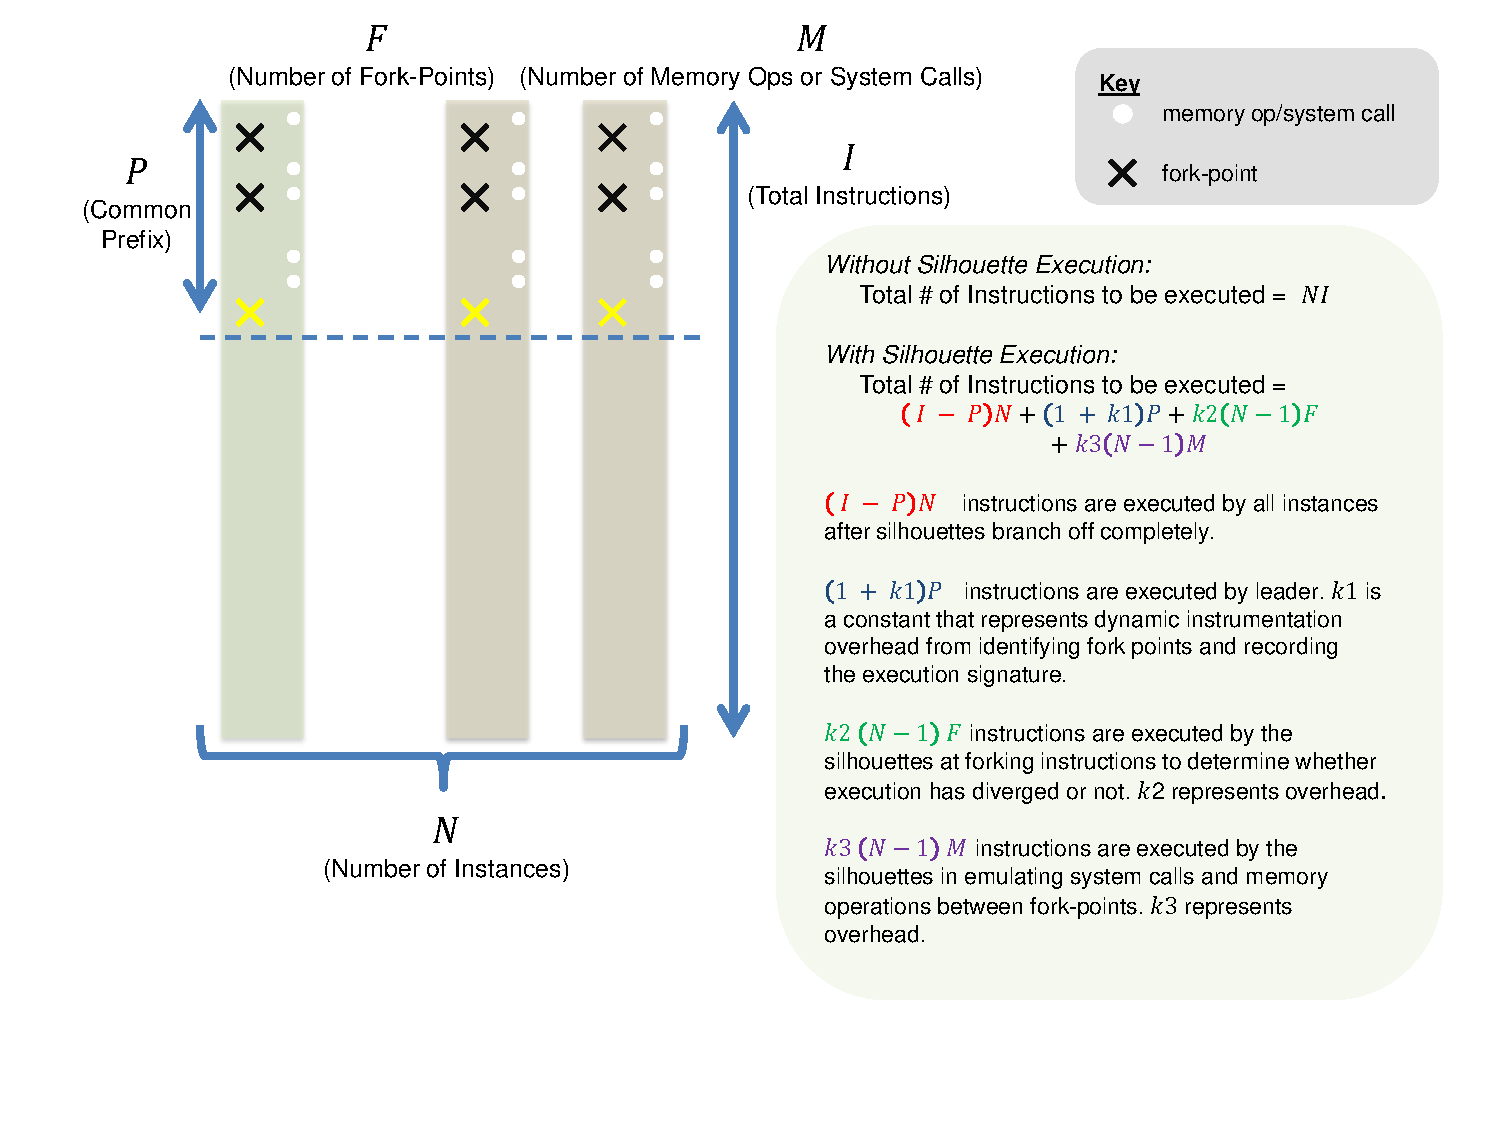
\includegraphics[scale=0.75, trim=3cm 0cm 1cm 0cm]{calc.pdf}
  \caption[Modeling CPU overhead from precise silhouetting]%
          {A simple way to model CPU overhead from precise silhouetting.
            We can compare the user-space instructions executed from running
            a program multiple times in the status quo
            versus the number of instructions executed
            when precise silhouetting is used for
            the same scenario. $k1$, $k2$ and $k3$ 
            are constants that represent overheads
            associated with this approach.}
  \label{psoverhead}
\end{figure}

\noindent {\bf Optimistic Silhouetting (Excluding Control Flow)} \newline 
Instructions in the longest common subsequence ($LCS$)
of multiple traces {\em before} a control flow
divergence broadly represent the savings from 
this variant of optimistic silhouetting.
Figure \ref{osncoverhead} summarizes how $T_{S}$ and $\vec K$ can be computed
for this variant of optimistic silhouetting. \newline

\begin{figure}
  \centering
  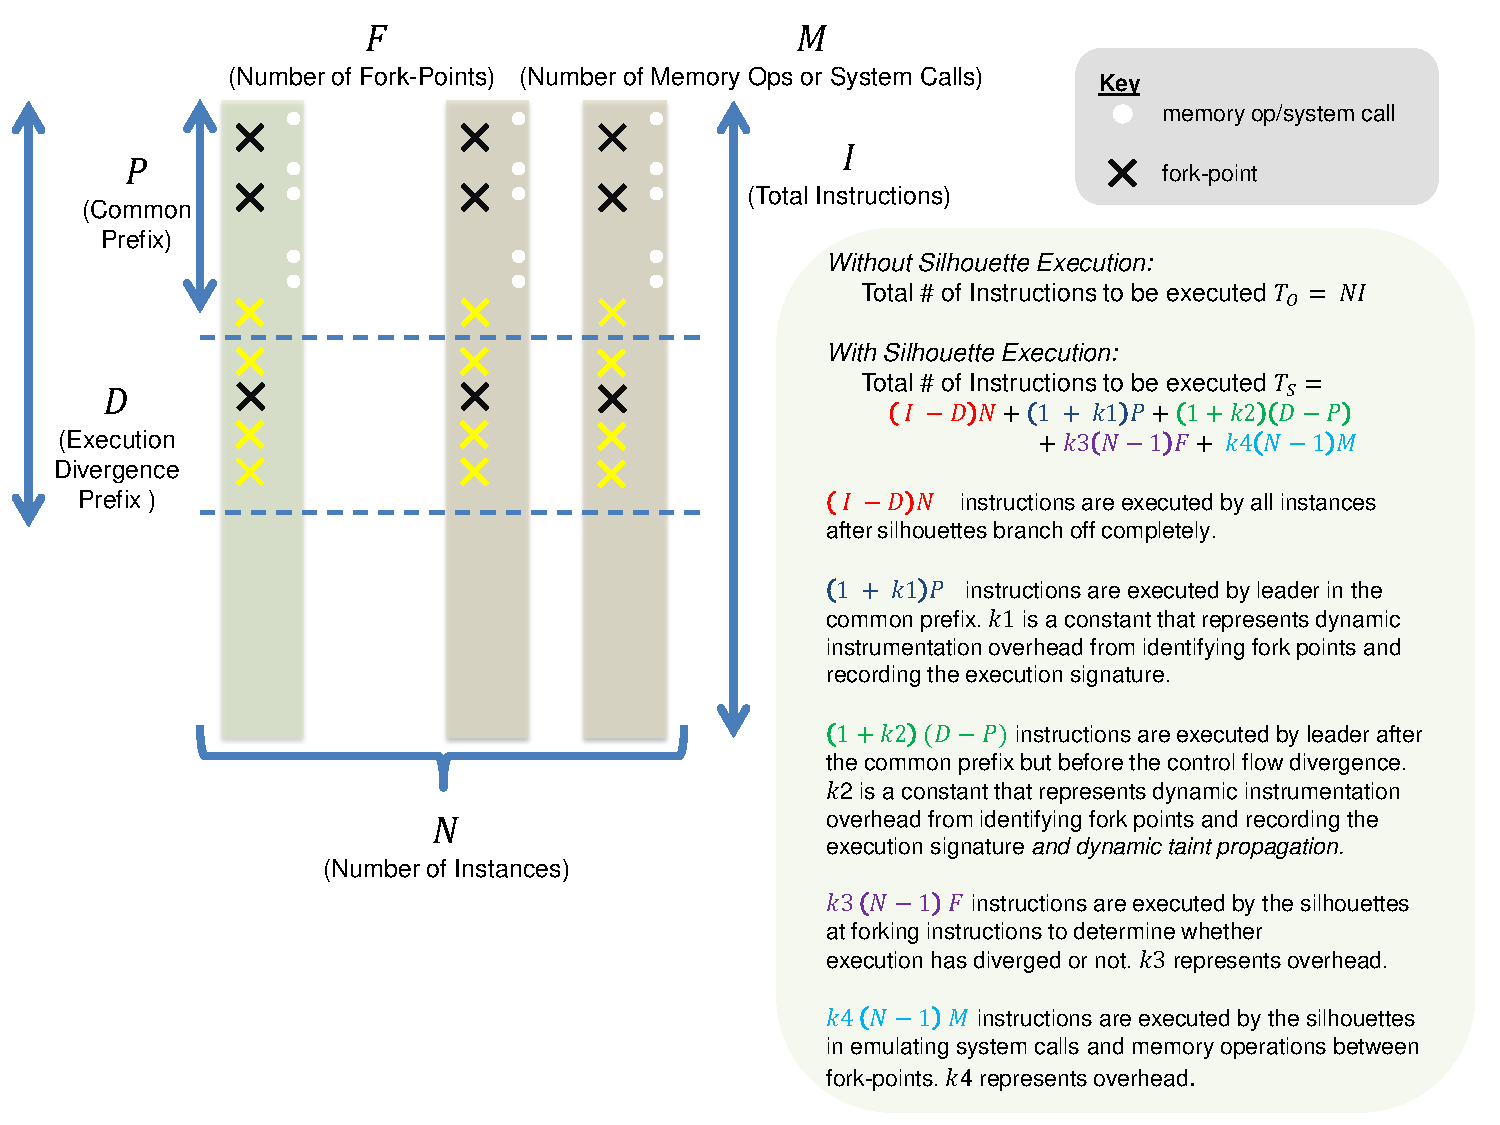
\includegraphics[scale=0.75, trim=3cm 0cm 1cm 0cm]{calc2.pdf}
  \caption[Modeling CPU overhead from optimistic silhouetting (excluding control flow)]%
          {A simple way to model CPU overhead from optimistic silhouetting (excluding control flow).
            We can compare the user-space instructions executed from running
            a program multiple times in the status quo
            versus the number of instructions executed
            when optimistic silhouetting is used for
            the same scenario. $k1$, $k2$, $k3$, and $k4$
            are constants that represent overheads
            associated with this approach.}
  \label{osncoverhead}
\end{figure}

\noindent {\bf Optimistic Silhouetting (Including Control Flow)} \newline
Instructions in the longest common subsequence ($LCS$)
of multiple traces before execution
diverges permanently represent the savings from 
this variant of optimistic silhouetting.
Figure \ref{oscoverhead} summarizes
how $T_{S}$ and $\vec K$ can be computed
for this design. 

\begin{figure}
  \centering
  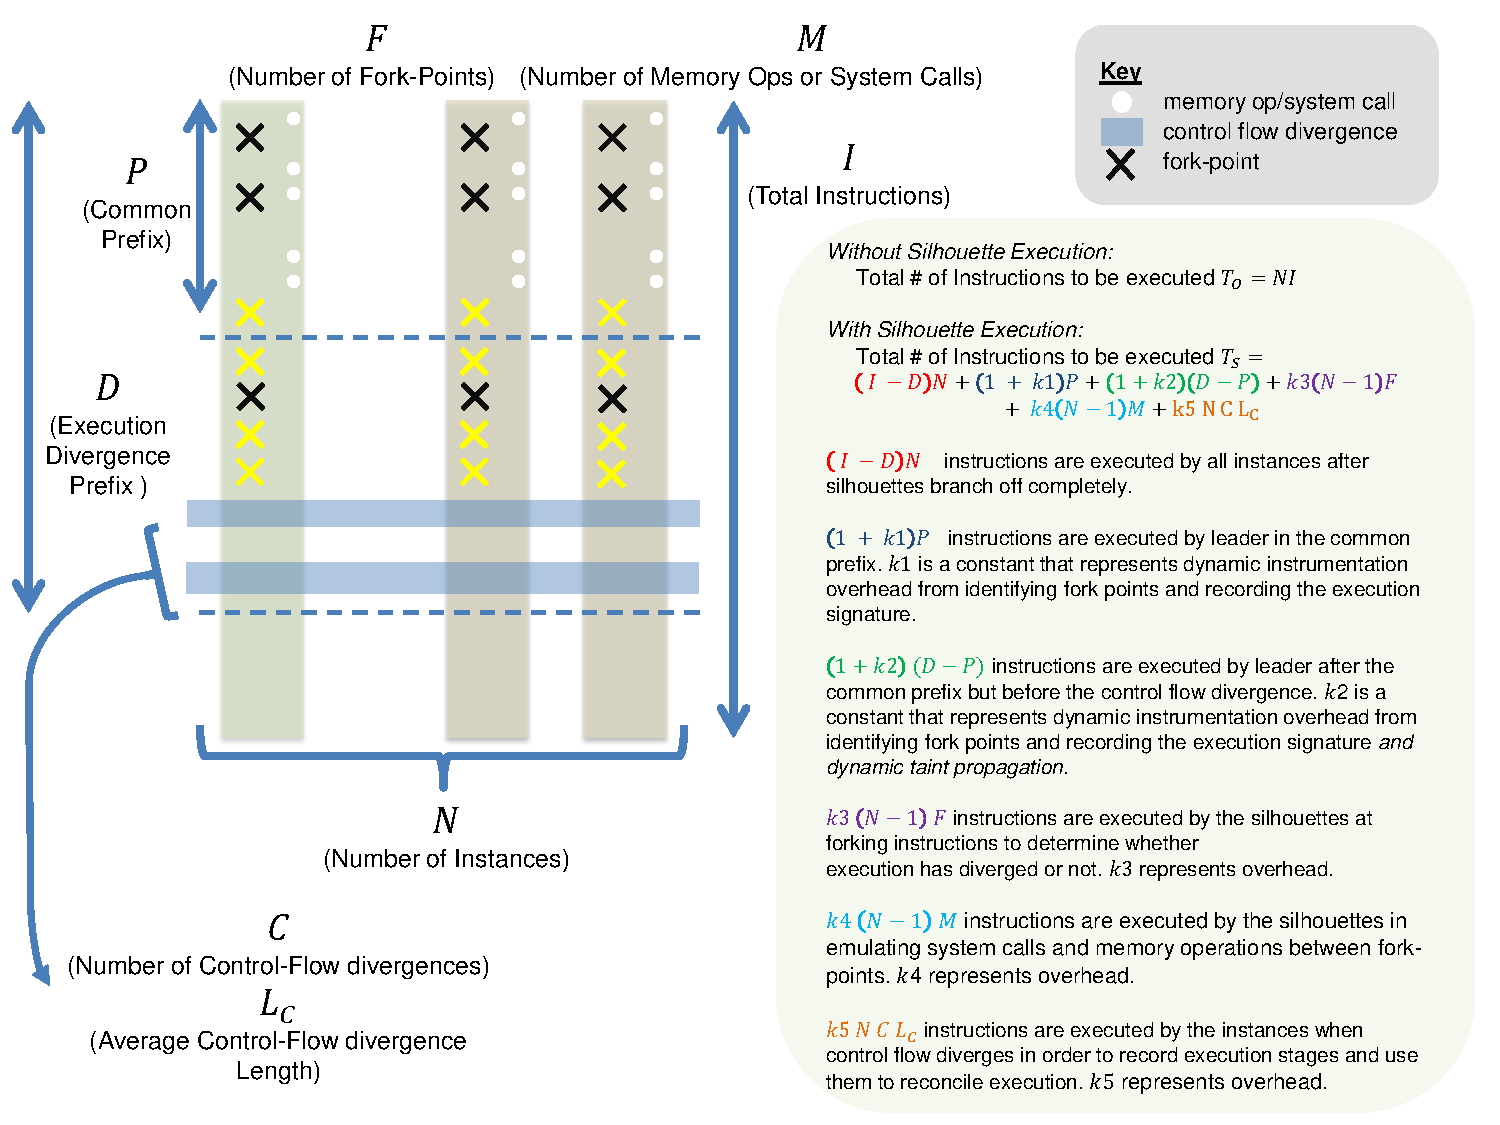
\includegraphics[scale=0.75, trim=3cm 0cm 1cm 0cm]{calc3.pdf}
  \caption[Modeling CPU overhead from optimistic silhouetting (excluding control flow)]%
          {A simple way to model CPU overhead from optimistic silhouetting (including control flow).
            We can compare the user-space instructions executed from running
            a program multiple times in the status quo
            versus the number of instructions executed
            when optimistic silhouetting is used for
            the same scenario. $k1$, $k2$, $k3$, $k4$ and $k5$ 
            are constants that represent overheads
            associated with this approach.}
  \label{oscoverhead}
\end{figure}

\subsection{Caveats}
Before we present our results, we
note a few limitations of our
methods for evaluating 
silhouette execution:

\begin{itemize}
\item We estimate the advantage ($A$) of silhouette execution
on user-space programs purely in terms of the 
number of instructions executed on the host CPU.
We do not model {\em latency} for silhouette
execution. It would be interesting
to study whether the delays introduced
by dynamic inspection of program execution and inter-instance communication
can eclipse the potential latency reduction from reduced CPU load
and bypassing execution in silhouette
execution or not. In practice,
the hypervisor layer 
rather than a dynamic instrumentation layer
would implement silhouette execution,
to reduce performance overhead.

\item Our dynamic instrumentation tool
can only inspect user-mode instructions
of the main process hosting an application,
so we cannot consider code
executed by lower software layers or other
children processes in computing $A$.
Overall, the number of instructions
we consider may be a fraction of all the
instructions computed on the host CPU,
which would add a dampening factor 
to our computed value of $A$.

\item 
The values we use for $\vec K$ are 
conservatively guessed, and
we assume the overheads from various
aspects of silhouette execution are linear in nature.
These assumptions, while reasonable, may understate
the CPU-load reduction practically attainable by silhouette
execution in user-space.

\item We do not factor the storage and I/O overhead
associated with the transmission of execution
signatures, though our experience
suggest that signature files are typically
very small (i.e. only a few megabytes)
so they should fit in host memory.

\item While we collect traces from many different silhouettes,
we simply pick the worst trace (i.e. the one with
the most difference from a leader) for computing
$T_S$. Thus, our models may be overly conservative because they assume that {\em all} 
silhouettes are as different from a leader as the {\em worst} silhouette.
This assumption simplifies the design and evaluation complexity related
from the leader having to handle silhouettes
with varying levels of divergence from
the leader.

\end{itemize}

Despite these limitations, we believe
that our model offers valuable insight
into the feasibility of silhouette execution
in user space because we instrument and evaluate
silhouette execution on large user-mode
instruction streams from Linux services,
and conservatively factor in the possible overhead
from silhouette execution.

\subsection{Initial Results}
\noindent {\bf Precise Silhouetting} \newline
Table \ref{ps:inittbl} shows the results of modeling 
precise silhouetting on a few Linux services.
For simplicity, we treat
all system calls as fork-points.
This assumption increases the number of fork-points ($F$);
it also increases the overhead associated with determining 
if execution has diverged or not after a fork-point
because the inspection layer has to presumably
understand the logic of each system call
to determine its side effects ($k2$). However,
this assumption reduces $k1$ because an overwhelming majority
of instructions that only use register operands are easily
excluded from fork-points. Instructions
that are system calls are also easily identifiable (i.e. \texttt{int 0x80} or \texttt{call *gs:0x10});
instructions with memory operands need
their memory addresses to be 
compared to tainted addresses (e.g. \texttt{gs:0x14} or \texttt{gs:0x18})
to determine whether they are fork points or not.
For our evaluation, we chose $k1 = 20$,
$k2 = 1000$ and $k3 = 20$ as reasonably
conservative values for the overhead constants.

\begin{table} [t]
\begin{center}
\begin{tabular}{|l||c|c||c||c|c|c||c||c|}\hline
  Program & $N$ & I & $T_O$ & $p$ & $M$ & $F$ & $T_S$ & $A$ \\\hline \hline
  \texttt{acpid} & 8 & 1.69\texttt{E}5 & 1.35\texttt{E}6 & 20.9\% & 4838 & 55 & 2.88\texttt{E}6 & 0.469 \\\hline
  \texttt{acpid} & 128 & 1.69\texttt{E}5 & 2.16\texttt{E}7 & 20.9\% & 4838 & 55 & 3.72\texttt{E}7 & 0.581 \\\hline
  \texttt{acpid} & 1024 & 1.69\texttt{E}5 & 1.73\texttt{E}8 & 20.9\% & 4838 & 55 & 2.94\texttt{E}8 & 0.589 \\\hline
  \hline

  \texttt{anacron} & 8 & 5.47\texttt{E}6 & 4.38\texttt{E}7 & 0.649\% & 4686 & 50 & 4.52\texttt{E}7 & 0.967  \\\hline
  \texttt{anacron} & 128 & 5.47\texttt{E}6 & 7.00\texttt{E}8 & 0.649\% & 4686 & 50 & 7.14\texttt{E}8 & 0.979  \\\hline
  \texttt{anacron} & 1024 & 5.47\texttt{E}6 & 5.60\texttt{E}9 & 0.649\% & 4686 & 50 & 5.71\texttt{E}9 & 0.967  \\\hline
  \hline

  \texttt{cron} & 8 & 2.31\texttt{E}6 & 1.84\texttt{E}7 & 1.54\% & 6329 & 60 & 2.02\texttt{E}7 & 0.912  \\\hline
  \texttt{cron} & 128 & 2.31\texttt{E}6 & 2.96\texttt{E}8 & 1.54\% & 6329 & 60 & 3.15\texttt{E}8 & 0.937  \\\hline
  \texttt{cron} & 1024 & 2.31\texttt{E}6 & 2.37\texttt{E}9 & 1.54\% & 6329 & 60 & 2.46\texttt{E}9 & 0.938  \\\hline
  \hline

  \texttt{cupsd} & 8 & 2.45\texttt{E}7 & 1.96\texttt{E}8 & 0.445\% & 20114 & 139 & 2.01\texttt{E}8 & 0.974  \\\hline
  \texttt{cupsd} & 128 & 2.45\texttt{E}7 & 3.14\texttt{E}9 & 0.445\% & 20114 & 139 & 3.19\texttt{E}9 & 0.982  \\\hline
  \texttt{cupsd} & 1024 & 2.45\texttt{E}7 & 2.51\texttt{E}10 & 0.445\% & 20114 & 139 & 2.56\texttt{E}10 & 0.983  \\\hline
  \hline

  \texttt{ntp} & 8 & 3.61\texttt{E}6 & 2.88\texttt{E}7 & 2.54\% & 11255 & 72 & 3.22\texttt{E}7 & 0.897  \\\hline
  \texttt{ntp} & 128 & 3.61\texttt{E}6 & 4.62\texttt{E}8 & 2.54\% & 11255 & 72 & 4.91\texttt{E}8 & 0.939  \\\hline
  \texttt{ntp} & 1024 & 3.61\texttt{E}6 & 3.69\texttt{E}9 & 2.54\% & 11255 & 72 & 3.92\texttt{E}9 & 0.942  \\\hline
  
\end{tabular}
  \caption{\hspace{0.2in}Preliminary Results from Modeling Precise Silhouetting.\newline 
    $A$, the advantage ratio is calculated by $\frac{T_O}{T_S}$.
    $T_O$ is the total instructions that would be executed in the status quo whereas $T_S$ is the total instructions that would be executed under
    precise silhouetting. $\vec K$ (not shown in the table), represents overhead constants and was selected conservatively
    to be $(20,1000,20)$. $M$ is the number of system calls and memory operations made by the leader before the first active fork-point; $F$
    is the number of latent fork-points before the first active fork-point. $p = 100P/I$ is
    the prefix ratio of the execution. }

\label{ps:inittbl}

\end{center}
\end{table}

Table \ref{ps:inittbl} shows that precise silhouetting has 
values for $A$ that are less than 1 for all of the Linux
services we sampled. In fact, $A$ is less than 1 regardless
of whether we consider 8, 128 or 1024 instances. 
The value of $A$ is close to 0.90 on average which represents a {\em degradation}
on CPU load i.e. precise silhouetting would execute more instructions
in user-space than the status quo.
Note that:
\begin{itemize}
\item Because $p$ is very small on average for our sample of Linux services, 
  execution diverges very quickly in the simulation. This explains
  why, for small values of $p$, we get values of $A$ that are very
  close to 1. There is little difference between 
  precise silhouetting with a small value of $p$ than
  the status quo.
\item The higher the value of $p$, the greater the degradation
  on CPU load. Thus, the longer precise silhouetting remains
  active, the worse results we get. For instance,
  \texttt{acpid} has a higher value of $p$ than the other
  services, and its value of $A$ is correspondingly smaller. 
  This means that precise silhouetting is ineffective
  in reducing CPU load because of the high overhead
  from executing the memory operations and fork-points.
\item The scheme exhibits some, but very limited
  scalability, again because of the small values of $p$.
  As the number of instances goes up, the values of $A$ 
  increase a little. For \texttt{acpid}, $A$ increases
  from 0.469 to 0.589 as the number of instances
  increases from 8 to 1024. However,
  for most services, the scalability is very limited
  and $A$ increases by very little as the number of instances
  goes up from 128 to 1024.
\end{itemize}

\noindent Thus, precise silhouetting, from our first 
evaluation, causes CPU load degradation. 
We need to find a way to reduce the overhead
from memory operations and fork-points,
and increase the prefix ratio $p$
to improve the values for $A$ and
the scalability of $A$ with respect to $N$,
the number of instances.

\newpage
\noindent {\bf Optimistic Silhouetting (Excluding Control Flow)} \newline
Table \ref{osnc:inittbl} shows the results of modeling 
optimistic silhouetting (without control flow) on our sample of Linux services.
As before, we treat all system calls as fork-points.
We use the same values of $k1 = 20$, $k3 = 1000$, $k4 = 20$
to model overheads from detection of fork-points in the leader,
comparisons of side-effects of forking instructions 
and emulation of system calls and memory writes in silhouettes respectively.
We use $k2 = 40$ to model the additional
overhead from taint propagation after the first
active fork-point.

\begin{table} [h]
\begin{center}
\begin{tabular}{|l||c|c||c||c|c|c||c||c|}\hline
  Program & $N$ & I & $T_O$ & $d$ & $M$ & $F$ & $T_S$ & $A$ \\\hline \hline
  \texttt{acpid} & 8 & 1.69\texttt{E}5 & 1.35\texttt{E}6 & 100\% & 16323 & 102 & 9.22\texttt{E}6 & 0.146 \\\hline
  \texttt{acpid} & 128 & 1.69\texttt{E}5 & 2.16\texttt{E}7 & 100\% & 16323 & 102 & 6.08\texttt{E}7 & 0.356 \\\hline
  \texttt{acpid} & 1024 & 1.69\texttt{E}5 & 1.73\texttt{E}8 & 100\% & 16323 & 102 & 4.45\texttt{E}8 & 0.388 \\\hline
  \hline

  \texttt{anacron} & 8 & 5.47\texttt{E}6 & 4.38\texttt{E}7 & 6.11\% & 36095 & 309 & 6.15\texttt{E}7 & 0.714  \\\hline
  \texttt{anacron} & 128 & 5.47\texttt{E}6 & 7.03\texttt{E}8 & 6.11\% & 36095 & 309 & 8.05\texttt{E}8 & 0.874  \\\hline
  \texttt{anacron} & 1024 & 5.47\texttt{E}6 & 5.63\texttt{E}9 & 6.11\% & 36095 & 309 & 6.36\texttt{E}9 & 0.886  \\\hline
  \hline

  \texttt{cron} & 8 & 2.31\texttt{E}6 & 1.84\texttt{E}7 & 98.12\% & 320075 & 814 & 1.43\texttt{E}8 & 0.129  \\\hline
  \texttt{cron} & 128 & 2.31\texttt{E}6 & 2.96\texttt{E}8 & 98.12\% & 320075 & 814 & 1.01\texttt{E}9 & 0.292  \\\hline
  \texttt{cron} & 1024 & 2.31\texttt{E}6 & 2.37\texttt{E}9 & 98.12\% & 320075 & 814 & 7.52\texttt{E}9 & 0.315  \\\hline
  \hline

  \texttt{cupsd} & 8 & 2.45\texttt{E}7 & 1.96\texttt{E}8 & 34.21\% & 1037608 & 1176873 & 8.85\texttt{E}9 & 0.022  \\\hline
  \texttt{cupsd} & 128 & 2.45\texttt{E}7 & 3.14\texttt{E}9 & 34.21\% & 1037608 & 1176873 & 1.54\texttt{E}11 & 0.020  \\\hline
  \texttt{cupsd} & 1024 & 2.45\texttt{E}7 & 2.51\texttt{E}10 & 34.21\% & 1037608 & 1176873 & 1.24\texttt{E}12 & 0.020  \\\hline
  \hline

  \texttt{ntp} & 8 & 3.61\texttt{E}6 & 2.88\texttt{E}7 & 15.08\% & 59853 & 3201 & 7.58\texttt{E}7 & 0.380  \\\hline
  \texttt{ntp} & 128 & 3.61\texttt{E}6 & 4.62\texttt{E}8 & 15.08\% & 59853 & 3201 & 9.71\texttt{E}8 & 0.475  \\\hline
  \texttt{ntp} & 1024 & 3.61\texttt{E}6 & 3.69\texttt{E}9 & 15.08\% & 59853 & 3201 & 7.65\texttt{E}9 & 0.482  \\\hline
  
\end{tabular}
\caption{Preliminary Results for Optimistic Silhouetting (Excluding Control Flow). \newline 
  $A$, the advantage ratio is calculated by $\frac{T_O}{T_S}$.
  The variables $T_O$, $T_S$, $M$, $F$ are the same as before (see Table \ref{ps:inittbl}).
  $d = 100D/I$ is the portion of the execution before the first control-flow divergence. }
\label{osnc:inittbl}
\end{center}
\end{table}

\noindent Because $d$ in Table \ref{osnc:inittbl} is significantly larger on average than $p$ in Table \ref{ps:inittbl},
we no longer get values of $A$ that are close to 1.0. The values of $A$ seen are much
lower than 1.0 (as low as 0.022 for \texttt{cups}); this indicates
that this version of optimistic silhouetting would lead to 
significant CPU performance {\em degradation}. This is largely
because of the increase in fork-points 
that result from tainted memory accesses,
and the high volume of memory operations that silhouettes
have to emulate.

\noindent {\bf Optimistic Silhouetting (Including Control Flow)} \newline
Table \ref{osc:inittbl} shows the results of modeling 
optimistic silhouetting (including control flow) on our sample of Linux services.
As before, we treat all system calls as fork-points. We use the same values of $k1 = 20$, $k2 = 40$, $k3 = 1000$, $k4 = 20$
to model overheads from detection of fork-points in the leader,
taint propagation, comparisons of forking instructions and
bypassing execution in silhouettes respectively.
We use $k5 = 20$ to model the additional
overhead from execution reconciliation
after a branch interval.


\begin{table} [h]
\begin{adjustwidth}{-1cm}{}
  \centering
  \begin{tabular}{|l||c|c||c||c|c|c|c|c||c||c|}\hline
    Program & $N$ & I & $T_O$ & $d$ & $M$ & $F$ & $C$ & $L_C$ & $T_S$ & $A$ \\\hline \hline
    \texttt{anacron} & 8 & 5.47\texttt{E}6 & 4.38\texttt{E}7 & 100\% & 7.2\texttt{E}5 & 26923 & 299 & 4 & 5.15\texttt{E}8 & 0.085  \\\hline
    \texttt{anacron} & 128 & 5.47\texttt{E}6 & 7.03\texttt{E}8 & 100\% & 7.2\texttt{E}5 & 26923 & 299 & 4 & 5.49\texttt{E}9 & 0.128  \\\hline
    \texttt{anacron} & 1024 & 5.47\texttt{E}6 & 5.63\texttt{E}9 & 100\% & 7.2\texttt{E}5 & 26923 & 299 & 4 & 4.26\texttt{E}10 & 0.132  \\\hline
    \hline
    
    \texttt{cron} & 8 & 2.31\texttt{E}6 & 1.84\texttt{E}7 & 100\% & 320075 & 1454 & 5 & 1 & 1.49\texttt{E}8 & 0.124  \\\hline
    \texttt{cron} & 128 & 2.31\texttt{E}6 & 2.96\texttt{E}8 & 100\% & 320075 & 1454 & 5 & 1 & 1.09\texttt{E}9 & 0.271  \\\hline
    \texttt{cron} & 1024 & 2.31\texttt{E}6 & 2.37\texttt{E}9 & 100\% & 320075 & 1454 & 5 & 1 & 8.14\texttt{E}9 & 0.291  \\\hline
    \hline
    
    \texttt{cupsd} & 8 & 2.45\texttt{E}7 & 1.96\texttt{E}8 & 100\% & 3.05\texttt{E}6 & 3.53\texttt{E}6 & 1432 & 89 & 2.62\texttt{E}10 & 0.008  \\\hline
    \texttt{cupsd} & 128 & 2.45\texttt{E}7 & 3.14\texttt{E}9 & 100\% & 3.05\texttt{E}6 & 3.53\texttt{E}6 & 1432 & 89 & 4.59\texttt{E}11 & 0.007  \\\hline
    \texttt{cupsd} & 1024 & 2.45\texttt{E}7 & 2.51\texttt{E}10 & 100\% & 3.05\texttt{E}6 & 3.53\texttt{E}6 & 1432 & 89 & 3.69\texttt{E}12 & 0.007  \\\hline
    \hline
    
    \texttt{ntp} & 8 & 3.61\texttt{E}6 & 2.88\texttt{E}7 & 100\% & 4.25\texttt{E}5 & 6.06\texttt{E}5 & 812 & 68 & 4.49\texttt{E}9 & 0.006  \\\hline
    \texttt{ntp} & 128 & 3.61\texttt{E}6 & 4.62\texttt{E}8 & 100\% & 4.25\texttt{E}5 & 6.06\texttt{E}5 & 812 & 68 & 7.89\texttt{E}10 & 0.005  \\\hline
    \texttt{ntp} & 1024 & 3.61\texttt{E}6 & 3.69\texttt{E}9 & 100\% & 4.25\texttt{E}5 & 6.06\texttt{E}5 & 812 & 68 &  6.35\texttt{E}11  & 0.005  \\\hline
  
  \end{tabular}
\end{adjustwidth}

\caption{Preliminary Results for Optimistic Silhouetting (Including Control Flow). \newline 
  We exclude \texttt{acpid} because it had no control flow differences.
  $A$, the advantage ratio is calculated by $\frac{T_O}{T_S}$.
  The variables $T_O$, $T_S$, $M$, $F$ are the same as before (see Table \ref{osnc:inittbl}). 
  $d = D/I$ is the portion of the execution before the first control-flow divergence. 
  $C$ and $L_C$ represent the number of control-flow divergences and their average length
  respectively.  $d = 100D/I$  the portion of the execution before permanent execution divergence. }
\label{osc:inittbl}

\end{table}

\noindent Because there is no permanent execution divergence, $d$ is 100\%
for our sample services. However, the values of $A$ are much lower than 1
partly because of the same factors as before: the number
of memory writes and fork-points is very high,
leading to prohibitively high overhead. Furthermore,
the overhead from bursty control flow divergences 
can also be a problem (as is the case for \texttt{cupsd} and
\texttt{ntp}).

\newpage
\section{Improving Silhouette Execution} \label{silimprove}
When we analyzed the execution
traces collected by our data collection scheme,
we found that several causes of execution
divergence across our sample
of Linux services were synthetic i.e. they were an artefact
of external sources of nondeterminism
rather than semantic differences in program execution.
We thus decided to introduce a deterministic
execution layer to our previous
designs to eliminate as many sources of 
fork-points as possible and to 
improve the feasibility
of silhouette execution.

\subsection{Modified Data Collection Scheme}
We modified our data collection scheme from Chapter \ref{ch:boot} 
(shown in Figure \ref{data:naive}) to simulate and
evaluate silhouette execution in the boot storm scenario.

\begin{figure}[]
  \center
  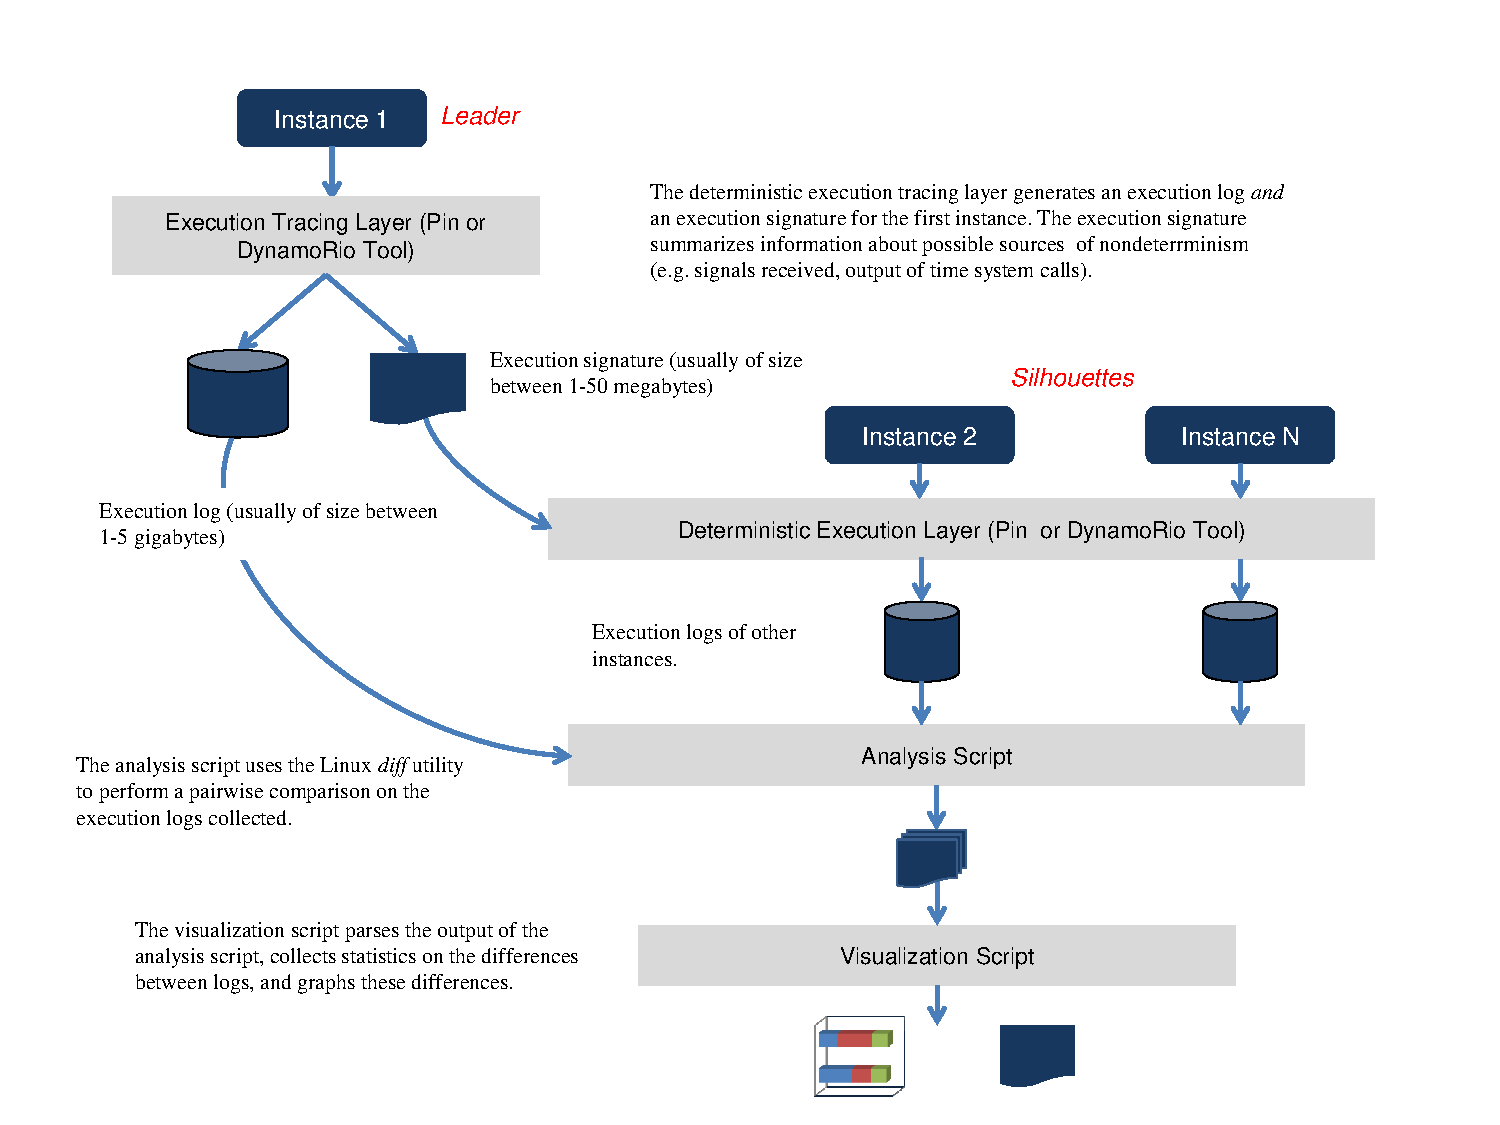
\includegraphics[scale=0.75, trim=2cm 0cm 1cm 0cm]
                  {simulation.pdf}
  \caption[Simulation of {\em Silhouette Execution} in a boot storm scenario]%
  {Simulation of {\em Silhouette Execution} in a boot storm scenario.
    We use dynamic instrumentation to 
    generate a trace signature file for the leader.
    While we do not bypass execution in the 
    silhouettes, try to reduce the number of fork-points 
    and record information about them.
    Our analysis and visualization
    scripts allow us to simulate and evaluate
    the effectiveness of {\em silhouette} execution.
  }
  \label{ch3:figsimulation}
\end{figure}


As shown by Figure \ref{ch3:figsimulation}, we run one instance of the
program -- the leader -- before all others.
For the leader, we generate an execution log, as before,
but we also augment the log by summarizing information about the sources of nondeterminism
described in Chapter \ref{ch:src}. For instance, we record
information about signal timing, process IDs, time-related system calls
in the trace signature file. Our Pin tool
uses the trace signature of the leader
to modify the instruction sequences executed by subsequent
executions (the silhouettes) and reduce the number of fork-points
as much as possible.

We run the leader to completion before the silhouettes.
As before, we also do not bypass instructions in silhouettes
so our modified data collection scheme still requires us
to analyze these traces to simulate and evaluate
silhouette execution.

\subsection{Reducing Execution Differences across Instances}
We now describe how we attempt to reduce
the source of execution differences from the sources described in Chapter \ref{ch:src}.
While we modify
the instances that execute after the leader, 
in practice many of our techniques eliminate fork-points altogether 
i.e. the leader can continue execution past
the forking instruction,
or avoid control flow differences by navigating
around variability of I/O timing and latency. \newline

%\noindent {\bf Address Space Layout Randomization (ASLR)} \newline
%Existing record-and-replay systems get around ASLR by
%forcing the operating system to use the same address space layout across
%different runs. A slightly more complex approach 
%would use base/offset computations to translate two equivalent 
%addresses between different executions. 
%For our experiments, we simply disabled ASLR using the command
%\texttt {sudo kernel.randomize\_va\_space=0} to simulate the 
%case where we nudge the operating system to construct
%similar address spaces for the same process. \newline

\noindent {\bf Canary and Pointer Guard Values} \newline
The values of the canary (\texttt{gs:0x14}) and the pointer guard (\texttt{gs:0x18})
are initialized in user-space, so dynamic instrumentation can be used to force 
these values to agree across distinct executions of the same program:
instructions that initialize them can be
modified or replaced; the sources used to compute
these values (e.g. \texttt{rdtsc}, \texttt{`/dev/urandom'}
or \texttt{AT\_RANDOM}) bytes
can be intercepted as well.

For a real implementation of silhouette execution, this means that a leader can simply choose to
not treat the instructions that initialize \texttt{gs:0x14} or
\texttt{gs:0x18} as fork-points and simply
treat them as normal memory writes instead. The silhouettes will follow the 
leader's execution signature and store the same canary or pointer guard
as the leader into memory. All subsequent instructions
that load the canary or pointer guard values 
from memory will also be identical and thus
will not be fork-points. 
\newline

\noindent {\bf Randomization} \newline
To overcome execution differences resulting from randomization,
we need to address the standard techniques
used by programs to seed PRNGs.
In our simulations, reads performed by the leader from \texttt{`/dev/urandom'}, the
\texttt{AT\_RANDOM} bytes, or the \texttt{rdtsc} instruction 
are intercepted and recorded in the trace execution file using
dynamic instrumentation;
for other subsequent instances, we simply
replace the return values to match
those from the leader.

For silhouette execution in practice, this means that the leader can simply
exclude \texttt{rdtsc} instructions 
or \texttt{read}s from \texttt{`dev/urandom'}
from fork-points and simply execute past them. 
Semantically, when silhouettes replay 
the leader's execution signature, this simulates
the unlikely but possible case that they
received the same random values as the leader
from external sources.

We need a slightly different approach for \texttt{AT\_RANDOM} bytes because they
are not initialized in user-space.
Simply excluding reads 
of \texttt{AT\_RANDOM} bytes from fork-points
is not sufficient for correctness:
when execution diverges permanently,
a silhouette may read \texttt{AT\_RANDOM}
bytes again and they will be different 
from those read earlier (which is impossible). 
To solve this minor issue, we can make the leader transmit
its \texttt{AT\_RANDOM} bytes
in its first execution signature;
the silhouettes overwrite
their own \texttt{AT\_RANDOM}
bytes with the leader's values
before starting execution.

These strategies eliminate
any fork-points or tainted memory
locations that result
from external
sources of randomization
in programs. While
eliminating such randomization
can change execution
semantics of a Linux service,
we are still simulating a valid
(and possible) execution path
for each silhouette. \newline

\noindent {\bf Time} \newline
In our simulations, 
system calls that return 
some measurement of the 
current time, the CPU or program execution time, or a time interval 
(e.g. \texttt{time} or \texttt{gettimeofday})
can be intercepted in the same manner
as randomization:
the timestamps logged
in the trace signature file
can be used to force agreement
between different instances.

For silhouette execution in practice, this means that a leader can simply
exclude such system calls from fork-points,
and continue executing past them. 
Rather than including these system calls in its
execution signature, the leader should include
the memory side-effects of these system calls.
This way, silhouettes do not perform these system calls; rather, they
automatically copy the behavior of the leader when they replay its 
writes. This simulates the unlikely 
but semantically valid scenario
that the various instances
executed various time-related system calls
precisely at the same times.
Replacing such system calls with their memory side-effects
works because they do not mutate any operating system
state.

The timestamps returned from
\texttt{stat} system calls
are not as easily handled. {\em If} we assume
that all the input, configuration
and data files are identical
between various instances of
a program, then we can 
simply exclude \texttt{stat}
system calls from fork-points
and include them 
in the execution signature file instead.
A leader can assume
by default that only the various timestamps
returned by \texttt{stat} will
be different and mark
them as tainted.
In our experiences,
these timestamps are typically
ignored in an overwhelming 
majority of cases. Thus, 
tainting these values by
default creates little overhead
because these values are seldom
read or propagated. At the same time,
we avoid the overhead associated
with treating \texttt{stat}
system calls as fork-points.

In the rare cases where
the timestamps from \texttt{stat}
system calls are actually read,
they are typically compared to
determine ``freshness''
(i.e. which file is newer).
When we assume that all
the files accessed by a program
have similar initial contents,
these comparisons can also
be excluded from 
fork-points because timestamps
retain the same ordering across different
instances of a program
in our experiments. This can be a risky
optimization, so to be absolutely sure, 
the leader could treat these comparisons as fork-points
and verify that the comparison results are the same
in all instances instead. 

To model this in our simulations, we do not include
\texttt{stat} system calls that contain
different time-stamps across instances in our
count of fork-points. However, comparisons of
timestamps from \texttt{stat} system
calls are included in our definition of fork-points.
\newline

\noindent {\bf Signal Delivery} \newline
In order to overcome the unpredictable timing and 
order of signals in our simulations, we intercept all signals received by 
an application and ensure they are delivered
at precisely the same instruction counts
and in the same order as that indicated
in the trace signature file.
Unlike record-and-replay systems, we only
deliver signals that are {\em actually}
received. Thus, signals that are received earlier
than expected are simply delayed or reordered. If,
however, a signal is not received at the expected
instruction count, our instrumentation tool
simply waits or inserts \texttt{nops} until the 
desired signal is received. If a signal simply
refuses to appear for a long time, execution
must diverge. In our experiments,
this final case does not occur as long
as other sources of nondeterminism are controlled. 

For silhouette execution in practice, this means that a leader can exclude
received signals from fork-points (unlike before),
and simply include them in the execution signature sent to silhouettes
instead. When silhouettes bypass execution using the execution signature,
they delay, reorder and deliver signals at precisely the 
same times as the leader and thus avoid any control-flow divergences. 
This technique, {\em signal alignment}, 
requires each silhouette to temporarily
resume execution from the instruction before which the signal is
expected to be received, and then insert \texttt{nops}
until the signal is received or deliver a previously
received (and withheld) signal.
This can prevent control
flow divergences and subsequent fork-points that arise from 
variable signal timing and ordering.
Of course, if the expected
signal is not received in a silhouette
within a reasonable time interval, 
control flow must inevitably diverge.
\newline

\noindent {\bf Process IDs} \newline
In our simulations, nondeterminism from process IDs
can be controlled by {\em virtualizing the process ID layer}, 
as shown by Figure \ref{ch3:pidfig}.
Using dynamic instrumentation, we can replace
real and unpredictable process IDs from kernel space
with virtual and unpredictable process IDs in user space.
As outlined in Section \ref{ch3:pid}, all interfaces
which use process IDs need to be carefully monitored
so that process IDs can be translated back and forth
for correctness. 

\begin{figure}[t]
  \center
  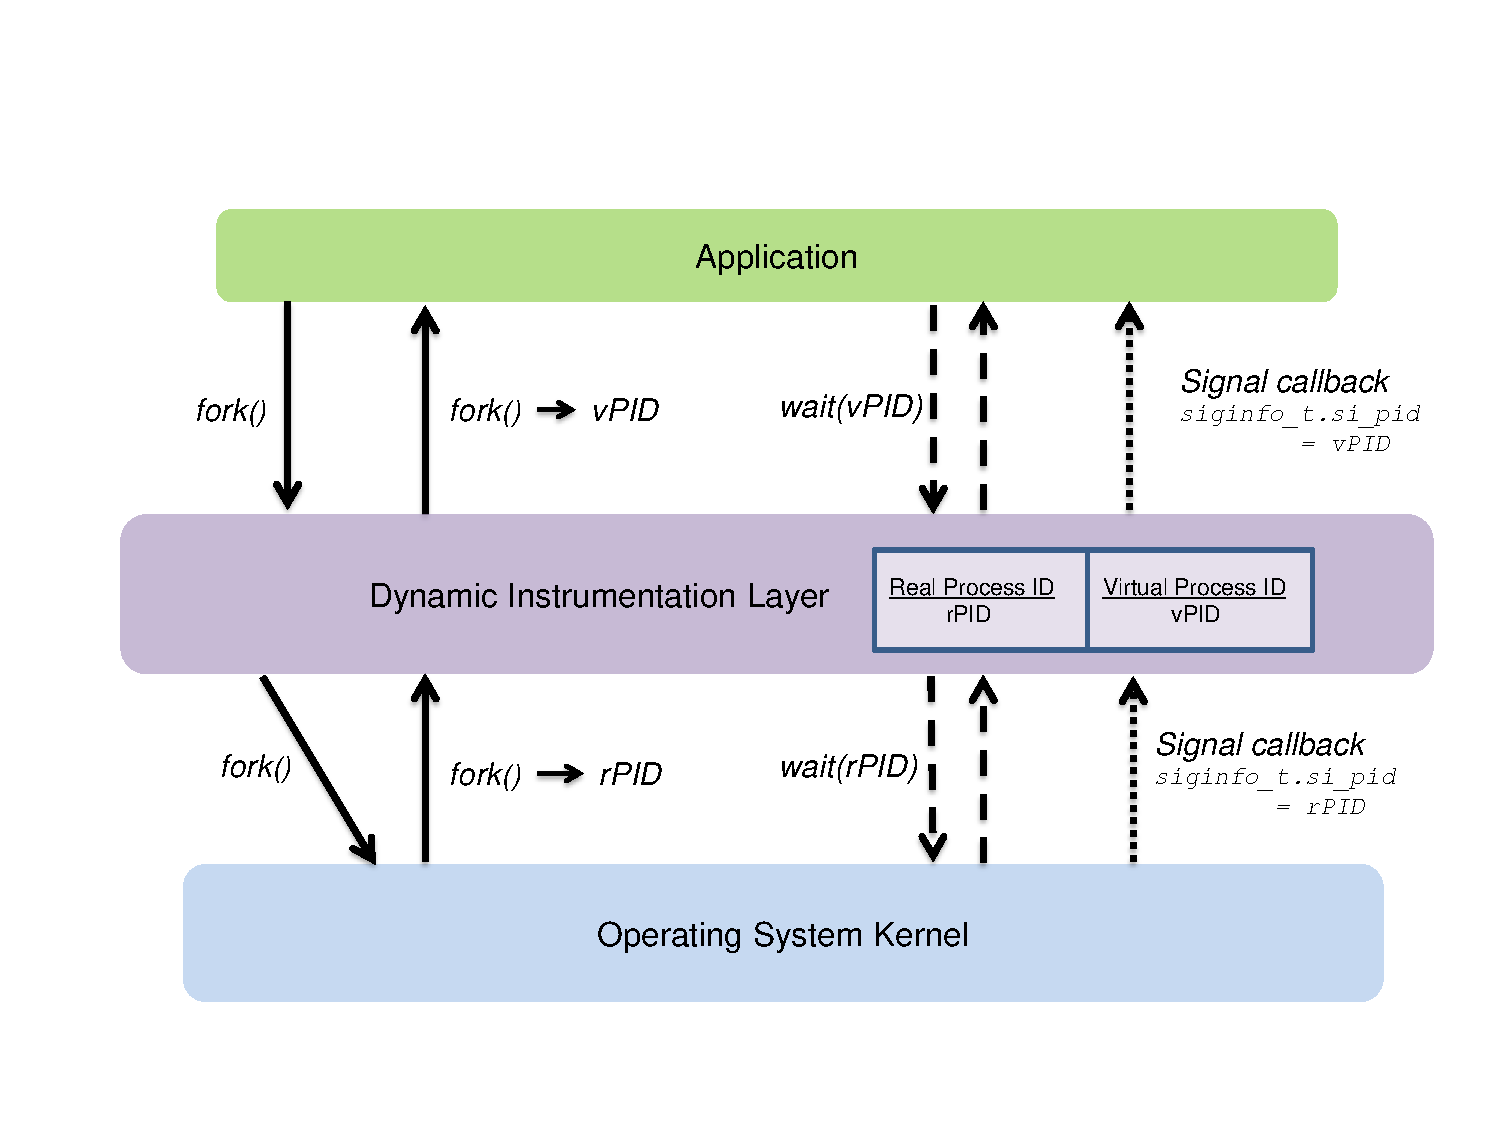
\includegraphics[trim=0cm 1cm 0cm 0.5cm, scale=0.60]{pid.pdf}
  \caption[Virtualizing the process ID layer using Pin]% 
  {All system calls and communications
  between the Linux user and kernel space are intercepted; 
  the dynamic instrumentation layer
  uses a PID translation table, and
  translates between real and virtual process IDs
  to ensure correctness. }
  
  \label{ch3:pidfig}
\end{figure} 

In practice, this is equivalent
to using an operating system that assigns
process IDs in a deterministic fashion.
In a complete implementation of silhouette
execution, we could expect the leader VM
to store process IDs in its execution 
signature; silhouettes would assign process IDs
in the same order as the leader.

For silhouette execution purely in 
user-space, we could add some logic to the silhouettes 
and virtualize their process IDs as described
in Figure \ref{ch3:pidfig}.
Instead of treating instructions that deal with process IDs as 
fork-points (e.g. \texttt{fork} or \texttt{clone}), the leader
would execute past them, and simply flag them before
including them in its execution signature.
When silhouettes would arrive at these 
instructions, they would simply translate
between real and virtual process IDs.
This clearly adds complexity and translation overhead
whenever an instance interacts 
with an operating system interface using 
virtual process IDs. However, virtualizing
the process ID layer prevents
a considerable number of user-space instructions 
that propagate differences
in process IDs (e.g. in \texttt{libc} or \texttt{pthreads}) from being labeled at fork-points
due to taint propagation.
Note that,  for correctness, silhouettes
must pretend to use the same virtual process IDs
that they have already used before even after they completely 
diverge execution.\newline

\noindent {\bf File I/O} \newline
Differences in input file contents across
executions would inevitably cause execution
to diverge, but reducing fork-points arising
from time, randomization or process ID system calls
is typically sufficient to ensure that
file contents evolve identically in Linux services. 
Some files that may differ
between two instances on start up (e.g. 
cache files or logs) can simply be 
deleted or replaced without sacrificing correctness.
Also, as mentioned already, \texttt{stat} 
timestamps are frequently not read, so
they can be excluded from fork-points until
they are actually compared with
other timestamps.

For file contents that are inherently and minimally different
(e.g. they contain different timestamps),
taint propagation otherwise suffices to ensure that 
they do not cause execution to diverge permanently. \newline

\noindent{\bf Network I/O} \newline
The content of network configuration files
does not change over a booting period in our experiments,
so we can mark them as immutable
during the boot process and
arrange for their \texttt{stat} timestamps
to return identical values across different
instances. In practice,
this means that a leader can 
exclude the \texttt{stat}
calls for network files
or their comparisons from its
set of fork-points without
sacrificing correctness.

In the same vein, the leader can exclude 
IP address resolution instructions from its definition
of fork-points, and execute past them. This disables DNS-based 
dynamic load balancing during the boot process and forces silhouettes
to use the same resolved IP addresses as the leader.
DNS-based load balancing typically uses low TTLs, so once 
the boot process is finished and execution diverges
permanently, the IP addresses will be refreshed 
quickly.

If bytes read from sockets differ across different executions,
we need to understand the {\em context} to determine whether the
differences are serious (e.g. due to different requests)
or synthetic (e.g. due to timestamps). Simply tainting 
the bytes that are different between
the instances is sufficient to tolerate
minor differences from external data.
In some specific cases, we can avoid marking
socket \texttt{read}s as fork-points:
for \texttt{Netlink} sockets, typically the only differences
in bytes across different instances
arise from interface statistics (\texttt{RTM\_NEWLINK}), 
sequence numbers or end-point IDs.
To handle variability in interface statistics (which are rarely read, if at all),
we can simply overwrite them with identical fixed values
across instances; sequence numbers
and end-points IDs are generated by 
\texttt{time} system calls and process IDs
respectively, which we already handle.
Thus, a leader can execute a socket 
\texttt{read} on \texttt{Netlink} sockets
and simply add memory operations that 
replace any statistics read by the silhouette
with what the leader read. 
This simulates the unlikely but semantically valid execution
scenario that all instances have the same network 
statistics (e.g. packets dropped/transmitted) when the 
system call is made.
Using this approach, while we introduce instrumentation overhead
in the leader for handling \texttt{Netlink} sockets, we reduce the number of expensive
fork-points requiring byte-by-byte comparisons related to \texttt{Netlink} socket \texttt{reads}
across all instances.

To overcome fork-points related to ephemeral port assignments, 
the leader can monitor the \texttt{bind} or \texttt{connect} 
system calls and changes their arguments to explicitly request ports
in the ephemeral range rather than let the kernel 
assign them. These system calls, then,
are no longer fork-points; the silhouettes
derive and use the same arguments as the leader from
the execution signature files sent to them,
so there are no execution differences.
This allows us to avoid virtualizing ephemeral ports
in a similar fashion to how we virtualize process IDs. \newline

\noindent{\bf Scalable I/O Schemes} \newline
To handle nondeterminism caused by unpredictable
ordering of I/O events,
we use techniques similar to those used 
for reordering signals in our simulations,
as described by Figure \ref{ch3:reorderfig}.
We name our approach {\em I/O stalling}.

\begin{figure}[h]
  \center
  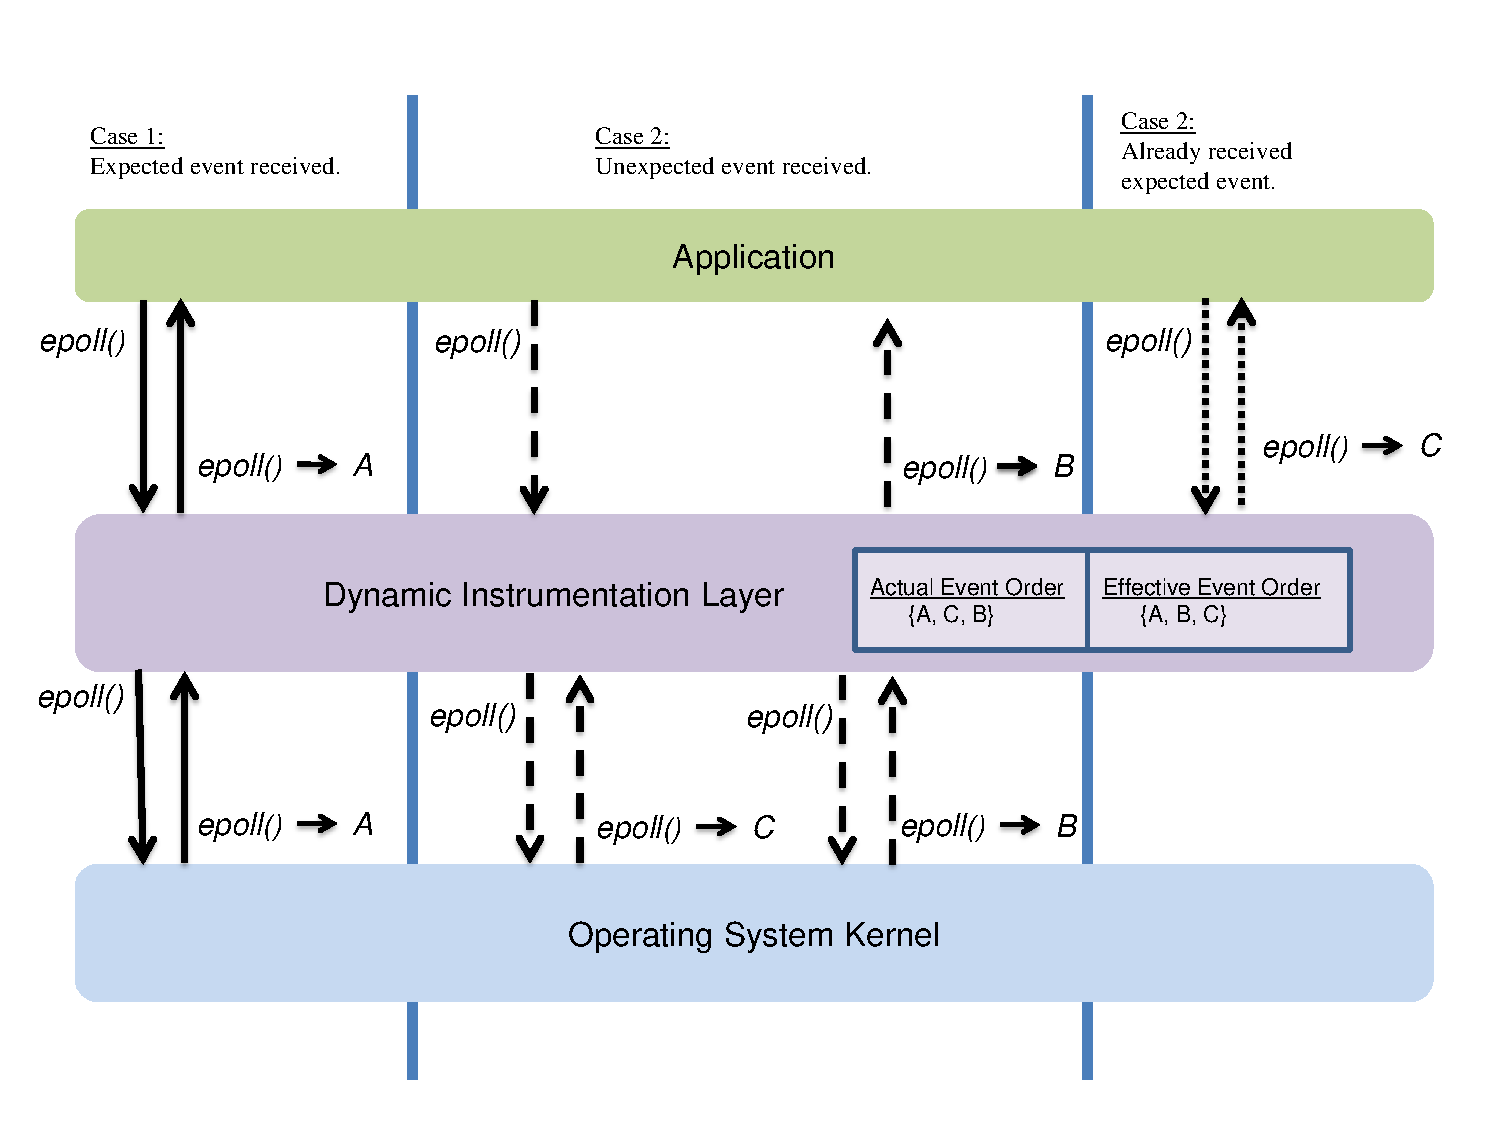
\includegraphics[trim=0cm 1.25cm 0cm 0.75cm, scale=0.60]{epoll.pdf}
  \caption[Reordering I/O events using Pin]% 
    {We intercept all \texttt{epoll} system calls,
    and use the execution signature file to
    achieve determinism. We do not ``replay'' I/O
    events because only events that actually do occur
    are delivered to the application instance. This
    diagram assumes \texttt{epoll} returns one event
    per call for the sake of illustration. }       
  \label{ch3:reorderfig}
\end{figure} 
              
Assuming that \texttt{epoll} returns just one event, figure
\ref{ch3:reorderfig} illustrates three possible cases that could occur:
\begin{itemize}
    \item The event returned by a call to \texttt{epoll} ($A$) is the one expected
    in the execution signature file ($A$). The instrumentation layer
    does not modify the system call.
    \item The desired event ($B$) has not been received yet,
    and \texttt{epoll} returns an unexpected event ($C$).
    The instrumentation layer stores the out-of-order event,
    and repeatedly calls \texttt{epoll} until the 
    the expected event is received.
    \item  A call to \texttt{epoll} is initiated, and the
    event desired ($C$) has already been received.
    The instrumentation layer does not 
    make a system call and simulates a return
    from \texttt{epoll} with the expected event instead.
\end{itemize}

Even if I/O events are reordered,
it is possible that different amounts
of data are available for ready
file descriptors across executions. We can 
mask this effect in the same
way we handle signals: if more bytes
are available (e.g. through \texttt{read}) 
than expected in the execution signature
file, we modify return values and \texttt{read}
buffers to delay the reading of these bytes
until the next \texttt{read}. In some corner
cases, we may have to ``fake'' readiness
in a call to \texttt{epoll}: if all bytes to be read from
a file descriptor have been read by 
the dynamic instrumentation layer (out of which
a few have not yet been delivered to the application),
there will be no more readiness events even
though the application expects them. If less-than-expected
bytes are available, we simply wait
till they are available by waiting for
another readiness update on the same file descriptor inside 
dynamic instrumentation layer.
In our experiments, this approach has been sufficient 
for overcoming nondeterminism from event-based I/O
schemes.
For asynchronous I/O schemes (e.g. \texttt{aio\_read}), strategies
similar to those used for reordering
and precisely-timing signals would be necessary to hide
variable I/O latency and ordering.

For silhouette execution in practice,
we would implement this technique -- {\em I/O alignment} -- by excluding \texttt{epoll} system calls
from fork-points. An \texttt{epoll}
call and its expected results
would be stored in the execution signature;
a silhouette would execute \texttt{epoll}
and not not let differences in the observed results 
let execution branch immediately. Instead,
the silhouette would repeatedly call
\texttt{epoll} until it gets the desired
event set, taking care to delay
and reorder I/O events as necessary
to align with the leader.
The same approach
can be used for determining 
how many bytes are available
from a \texttt{read}. While this 
adds overhead to the instructions
executed by a silhouette, it eliminates control-flow 
divergences and subsequent fork-points created from
inherent I/O nondeterminism. \newline

\noindent {\bf Concurrency} \newline
Execution variability resulting from multi-threading
has been extensively documented; there
is a significant body of work that
attempts to overcome such nondeterminism
by using deterministic logical clocks
or record-and-replay approaches. 
For our experiments, we did not attempt to enforce
a total order on the instructions executed in multi-threaded
programs and just measured fork-points inside 
the main process for each Linux service.
To reduce fork-points from multi-threading, we could incorporate
deterministic logical clocks 
into our design.

As mentioned before, a nondeterministic system scheduler
can cause variable timing of signals or I/O events, which
we handle using signal and I/O alignment strategies. 
Work on deterministic operating systems can
be extended to overcome this issue
in a more systematic manner. \newline

\noindent {\bf {\em Procfs}: The \texttt{`/proc/directory'}} \newline
A leader can exclude reads from {\em procfs}
for statistics from fork-points; instead, the leader can simply replace
them with memory operations that simulate
identical results in silhouettes. A leader
must be careful to flag reads from {\em procfs}
use process IDs, so that silhouettes
can translate between real and virtual process IDs
accordingly.

\newpage
\section{Evaluation of Improved Silhouette Execution} \label{sileval}
In this section, we evaluate the effectiveness of some of the techniques
introduced earlier to increase determinism in Linux services.
The next few subsections analyze some of 
the Linux services we sampled in our experiments
individually.

Tables \ref{evalsummarytbl1} and \ref{evalsummarytbl2} summarize the results of our experiments
using the modified data collection scheme. When we pick very high values for the overhead constants (represented by $\vec K$),
our techniques yield an aggregate improvement of 5.33$\times$
in the advantage ratio $A$ for 1000 VMs. That is, 
we go from a CPU load {\em increase} of 6\% due
to silhouette execution to a CPU load {\em reduction} by a 
{\em factor} of 4.772$\times$. When we pick reasonably conservative
values of $\vec K$ in our simulations, our techniques boost $A$ by a factor of 19.01$\times$,
and theoretically reduce the CPU load by a factor of 19.18$\times$.
Figure \ref{sumresults} visually graphs such improvements 
in $A$ over different values of $N$.

\begin{table} [h]
\begin{center}
\begin{tabular}{|l||c|c||c||}\hline
  Program & Preliminary Best $A$ & Current Best $A$ & Relative Improvement \\\hline \hline
  \texttt{acpid} & 0.589 & 1.16 & 1.96$\times$  \\\hline  
  \texttt{anacron} & 0.980 & 10.26 & 10.47$\times$  \\\hline  
  \texttt{cron} & 0.938 & 4.24 & 4.53$\times$  \\\hline
  \texttt{cupsd} & 0.982 & 5.91 & 6.02$\times$  \\\hline
  \texttt{ntpd} & 0.942 & 2.04 & 2.17$\times$  \\\hline \hline 
  \textbf{Average} & \textbf{0.886} & \textbf{4.772} & {\bf 5.33$\times$}  \\\hline
\end{tabular}
\caption{Improvements in $A$ for Linux services
  when $N = 1000$ and $\vec K$ is 
  picked conservatively i.e. $\vec K = (20, 1000, 20, 40, 1000)$.}
\label{evalsummarytbl1}
\end{center}
\end{table}

\begin{table} [h]
\begin{center}
\begin{tabular}{|l||c|c||c||}\hline
  Program & Preliminary Best $A$ & Current Best $A$ & Relative Improvement \\\hline \hline
  \texttt{acpid} & 1.031 & 6.20 & 6.01$\times$  \\\hline  
  \texttt{anacron} & 1.01 & 37.92 & 37.90$\times$  \\\hline  
  \texttt{cron} & 0.999 & 17.39 & 17.41$\times$  \\\hline
  \texttt{cupsd} & 0.999 & 24.31 & 24.33$\times$  \\\hline
  \texttt{ntpd} & 1.006 & 10.09 & 10.03$\times$  \\\hline \hline 
  \textbf{Average} & \textbf{1.009} & \textbf{19.18} & {\bf 19.01$\times$}  \\\hline
\end{tabular}
\caption{Improvements in $A$ for Linux services
  when $N = 1000$ and $\vec K$ is 
  picked less conservatively i.e. $\vec K = (10, 100, 5, 20, 50)$.}
\label{evalsummarytbl2}
\end{center}
\end{table}


\begin{figure}
  \centering
  \subfloat%[Part 1]
           {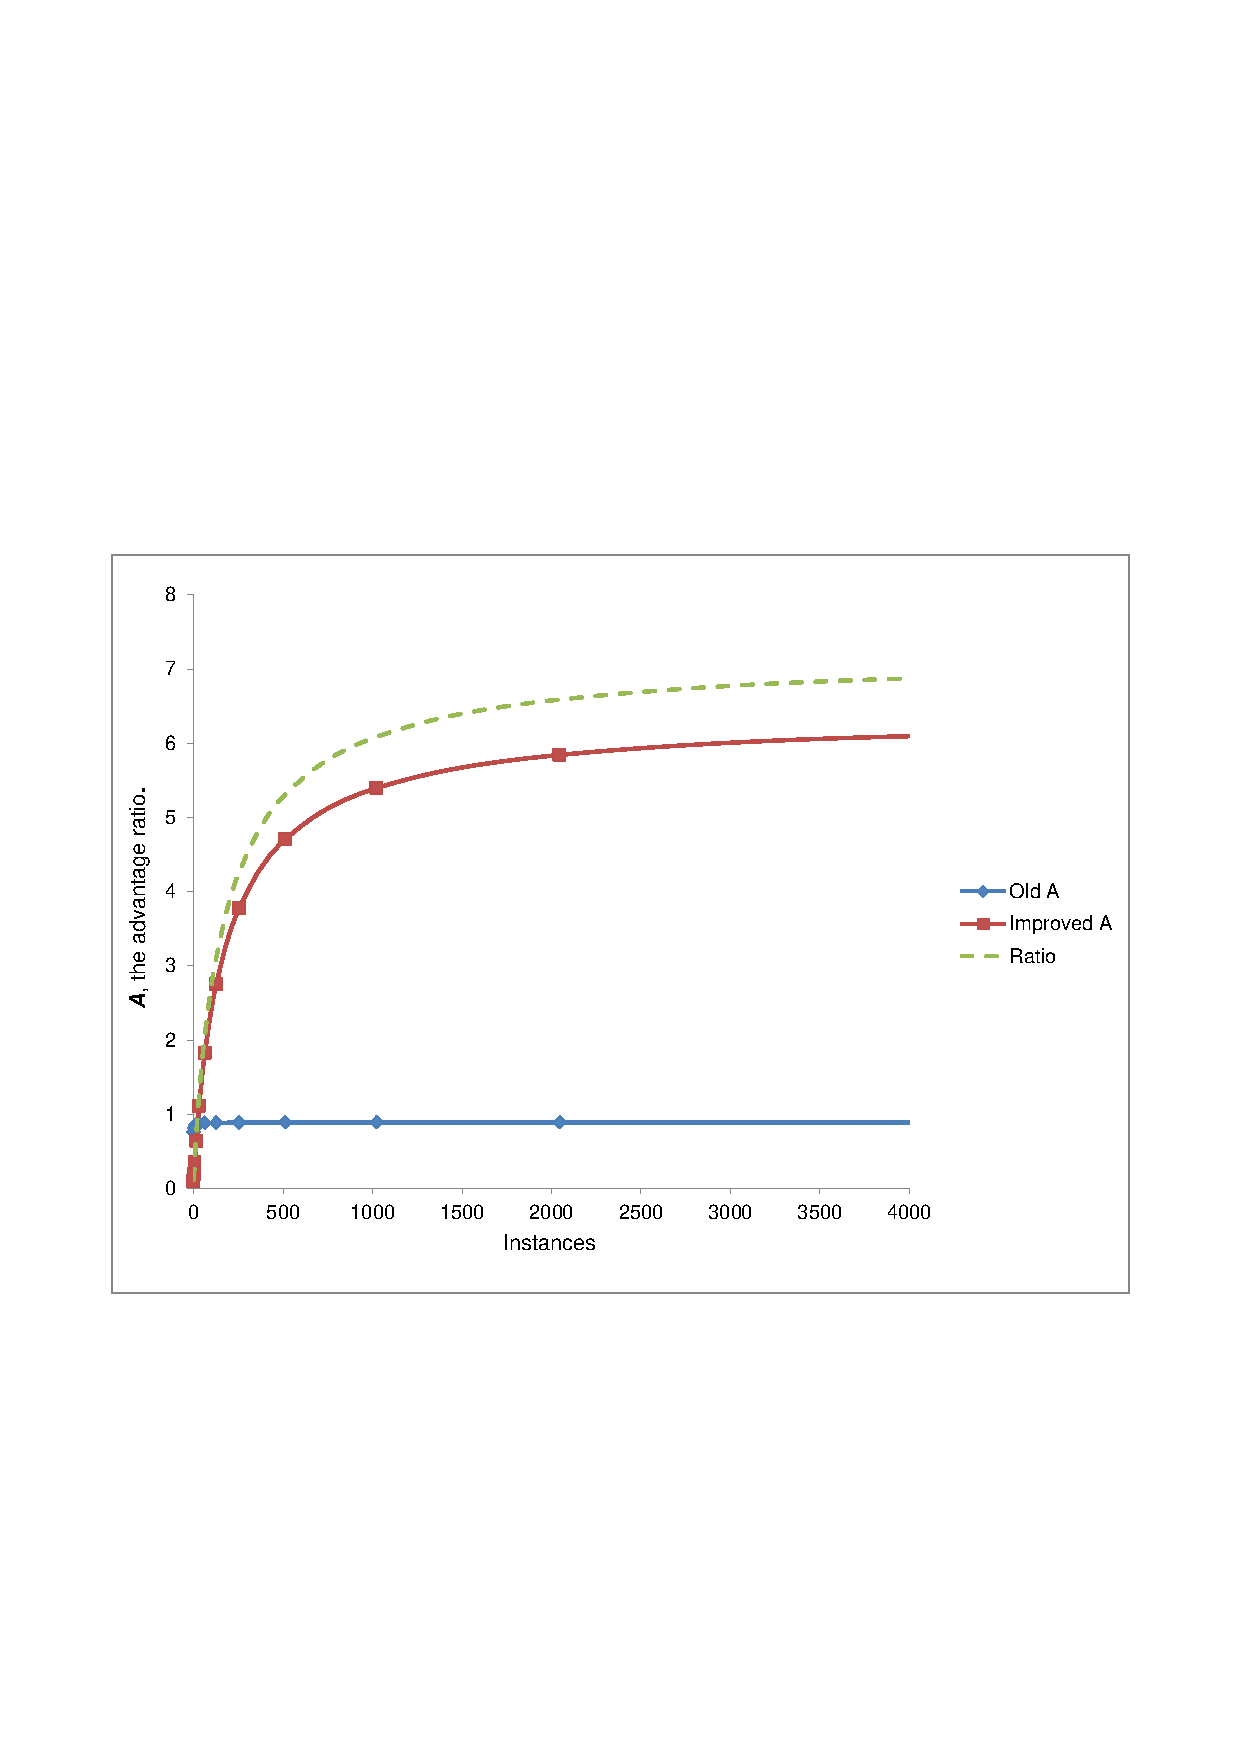
\includegraphics[scale=0.85, trim=5cm 8.5cm 5cm 10cm]{results1.pdf} \label{results1}} \\
  \subfloat%[Part 2]
      {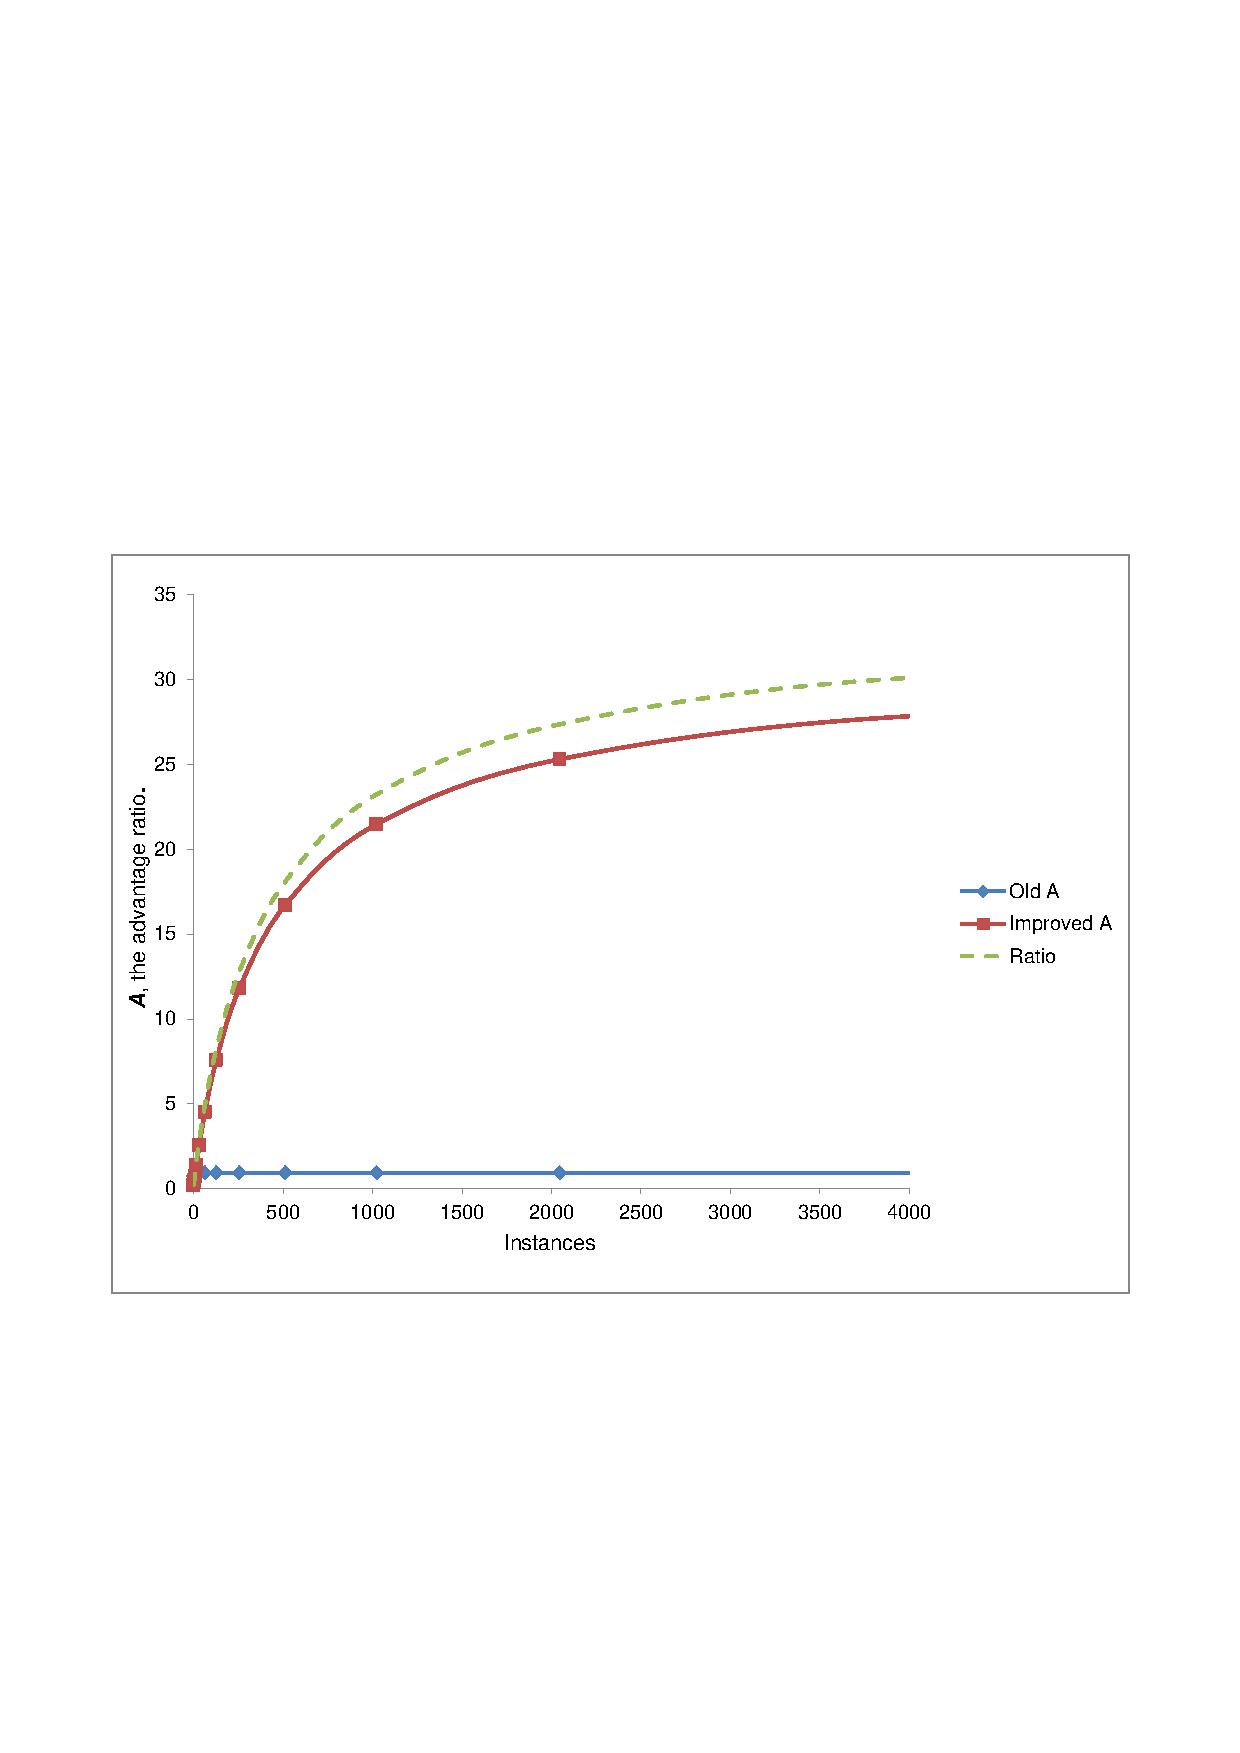
\includegraphics[scale=0.85, trim=5cm 8cm 5cm 8cm]{results2.pdf} \label{results2}} 
  \caption[Improvements in $A$ after controlling nondeterminism in Linux services.]%
          {Improvements in $A$ after controlling nondeterminism in Linux services.
          $\vec K$ for the top graph is much more conservative than that for the bottom graph.}

  \label{sumresults}
\end{figure}

\subsection{\texttt{acpid}}
The program {\texttt{acpid}} is a user-space daemon
typically launched at boot and is part of the Advanced Configuration
and Power Interface (ACPI) implementation in Linux.
The daemon listens for specific events triggered by 
external actions (e.g. pressing the power button, unplugging the AC adapter from
a notebook, or closing the notebook lid). When an event occurs,
it executes programs to handle that event (which
are specified through some configuration files).

\begin{figure}[h]
  \center
  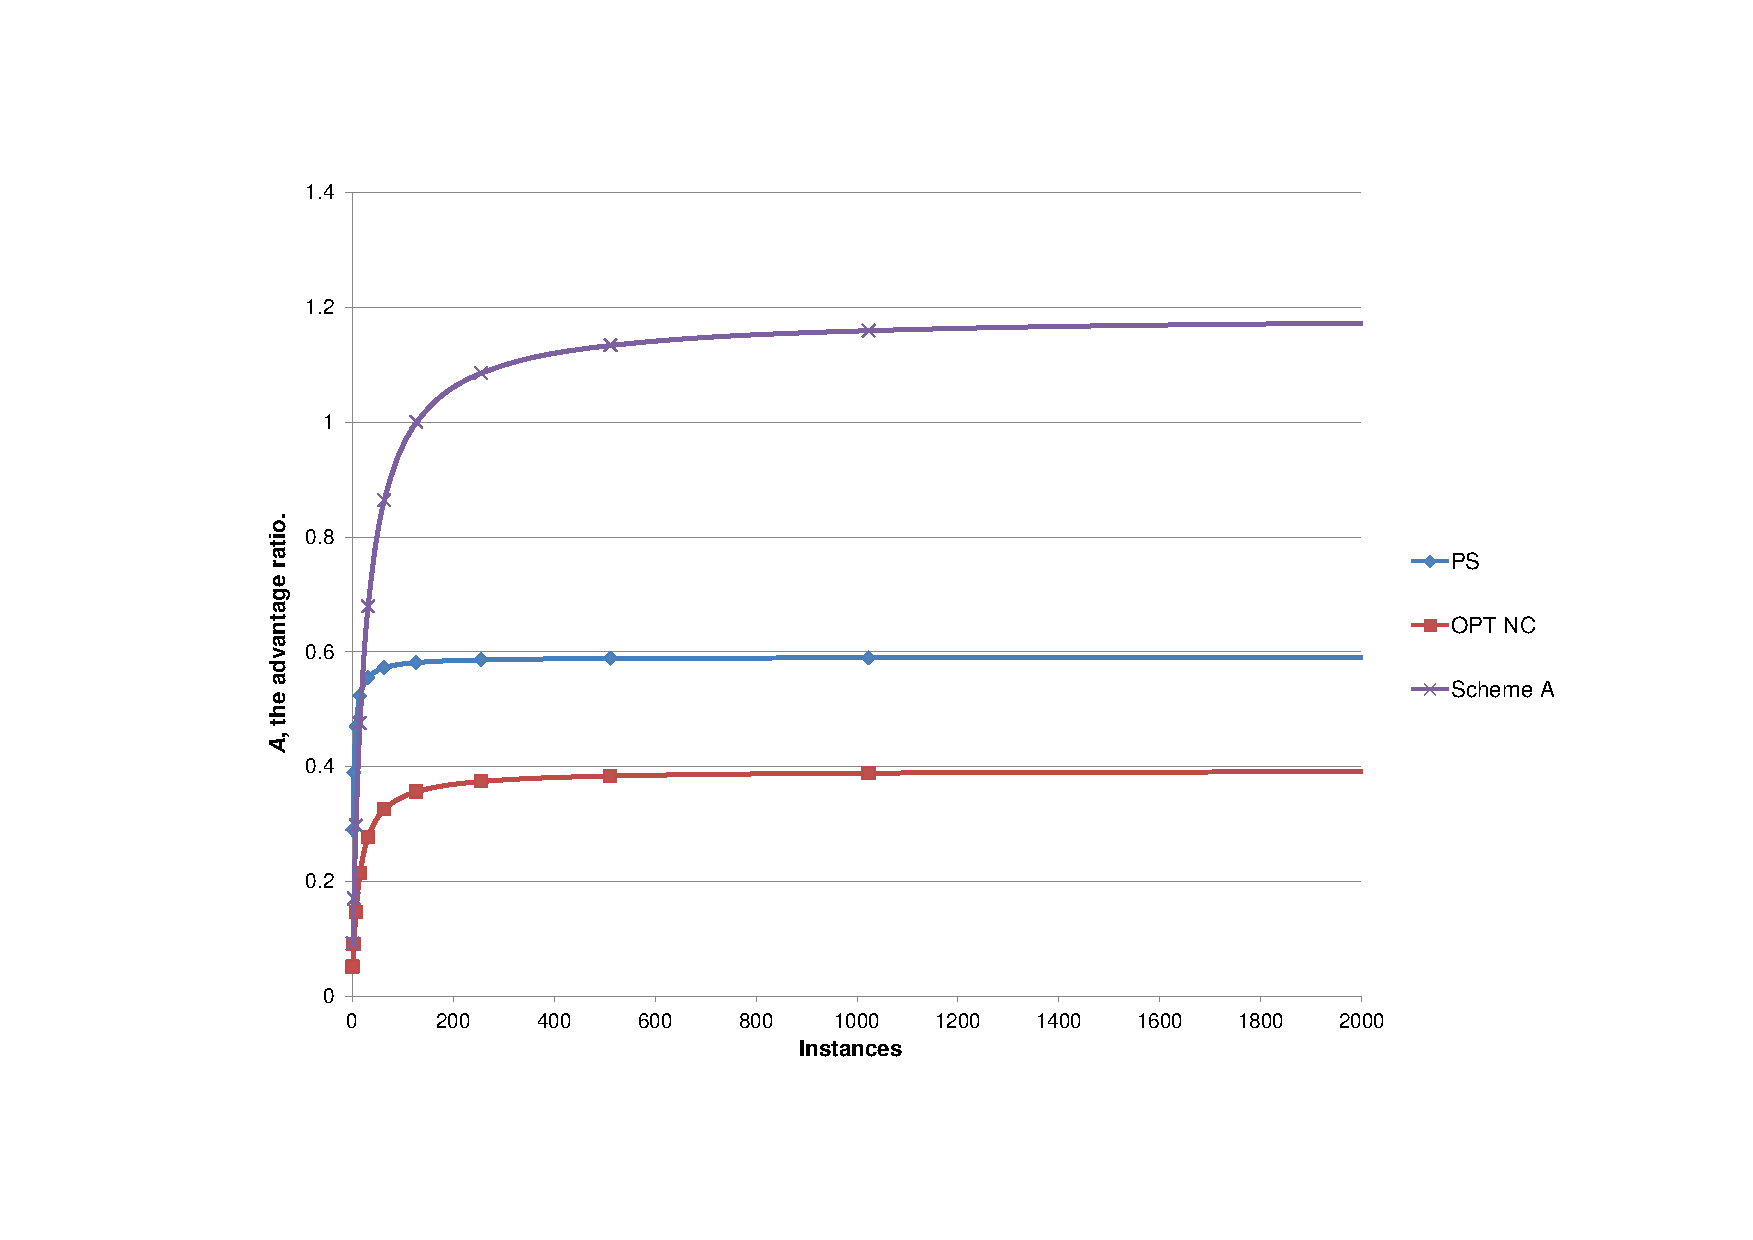
\includegraphics[scale=0.80, trim=5cm 3cm 0cm 3cm]{acpid-1.pdf}
  \caption[For \texttt{acpid}, $A$ as a function of $N$ (highly conservative $\vec K$)]% ]%
          {
            For \texttt{acpid}, computing $A$ as a function of $N$ (highly conservative $\vec K$).\newline
            \texttt{PS} and \texttt{OPT NC} are lines for precise silhouetting and optimistic 
            silhouetting (excluding control flow) without any improvements; they
            serve as a baseline to measure the success of our techniques
            in our simulations. \texttt{Scheme A} represents the improved values of $A$
            achieved through deterministic silhouette execution. There is no
            \texttt{OPT C} line for optimistic silhouetting (including 
            control flow) because there were no control flow divergences 
            in our \texttt{acpid} traces.
          }
  \label{acpid1}
\end{figure}

\newpage
\noindent Figure \ref {acpid1} shows the results of our experiments
to measure any improvements in $A$ from the techniques described in Section \ref{silimprove}.
Our workload consisted of simple boot-time initialization of \texttt{acpid}
i.e. a few iterations of its main loop. 

\texttt{Scheme A} includes the techniques we described to reduce
execution differences that arise from randomization, security and time;
these are sufficient to eliminate active fork-points in \texttt{acpid}
entirely. Thus, \texttt{Scheme A} uses precise silhouetting
in which execution does not diverge till the very end of our workload.
Unlike the baseline executions, \texttt{Scheme A} also simulates {\em write compression}:
silhouettes only write the latest values to memory locations instead of wastefully
replaying all intermediate writes  in {\em execution signatures}.

As shown in Figure \ref{acpid1}, \texttt{Scheme A} improves $A$ and
takes it above 1, converting a CPU load {\em increase}
into a CPU load reduction. However, the value of $A$ is not high
and does not scale too well as $N$ increases;
this is because of the high design overhead 
modelled by a highly conservative $\vec K$. In fact, the overhead 
in \texttt{acpid} from comparing forking instructions across instances, and replaying system calls and memory writes
across silhouettes is equally significant, unlike
the overhead from simply detecting fork-points.
Setting one of $k2$ or $k3$ to 0 immediately boosts $A$ by a factor of 2 for large $N$;
this factor is small because of generally high design overhead.

Figure \ref{acpid23} shows how $A$ changes with $N$ when we pick less conservative
values of overhead constants ($\vec K$) i.e. (10, 100, 5, 20, 50) 
rather than (20, 1000, 20, 40, 100). The achieved values of $A$ 
exceed 6 for $N < 1000$, which represents a significant
theoretical reduction in the number of user-space instructions
executed. The value of $A$ scales well for small $N$
(Figure \ref{acpid2}).
However, as $N$ increases, $A$ plateaus because some
of the design overhead (e.g. executing forking instructions or system
calls in the execution signature) grows with $N$. 

The highest theoretically possible
$A$ for our sampled traces is given by $A_{MAX} = \frac{I}{F+M}$,
which models the possibility that each instance only
executes system calls and {\em compressed} memory-writes
rather than $I$ instructions. For our samples of \texttt{acpid}, $A_{MAX}$ 
is about 40, and we get within a factor of 10 of that number in Figure \ref{acpid3}. 

\begin{figure}
  \centering
  \subfloat%[Part 1]
           {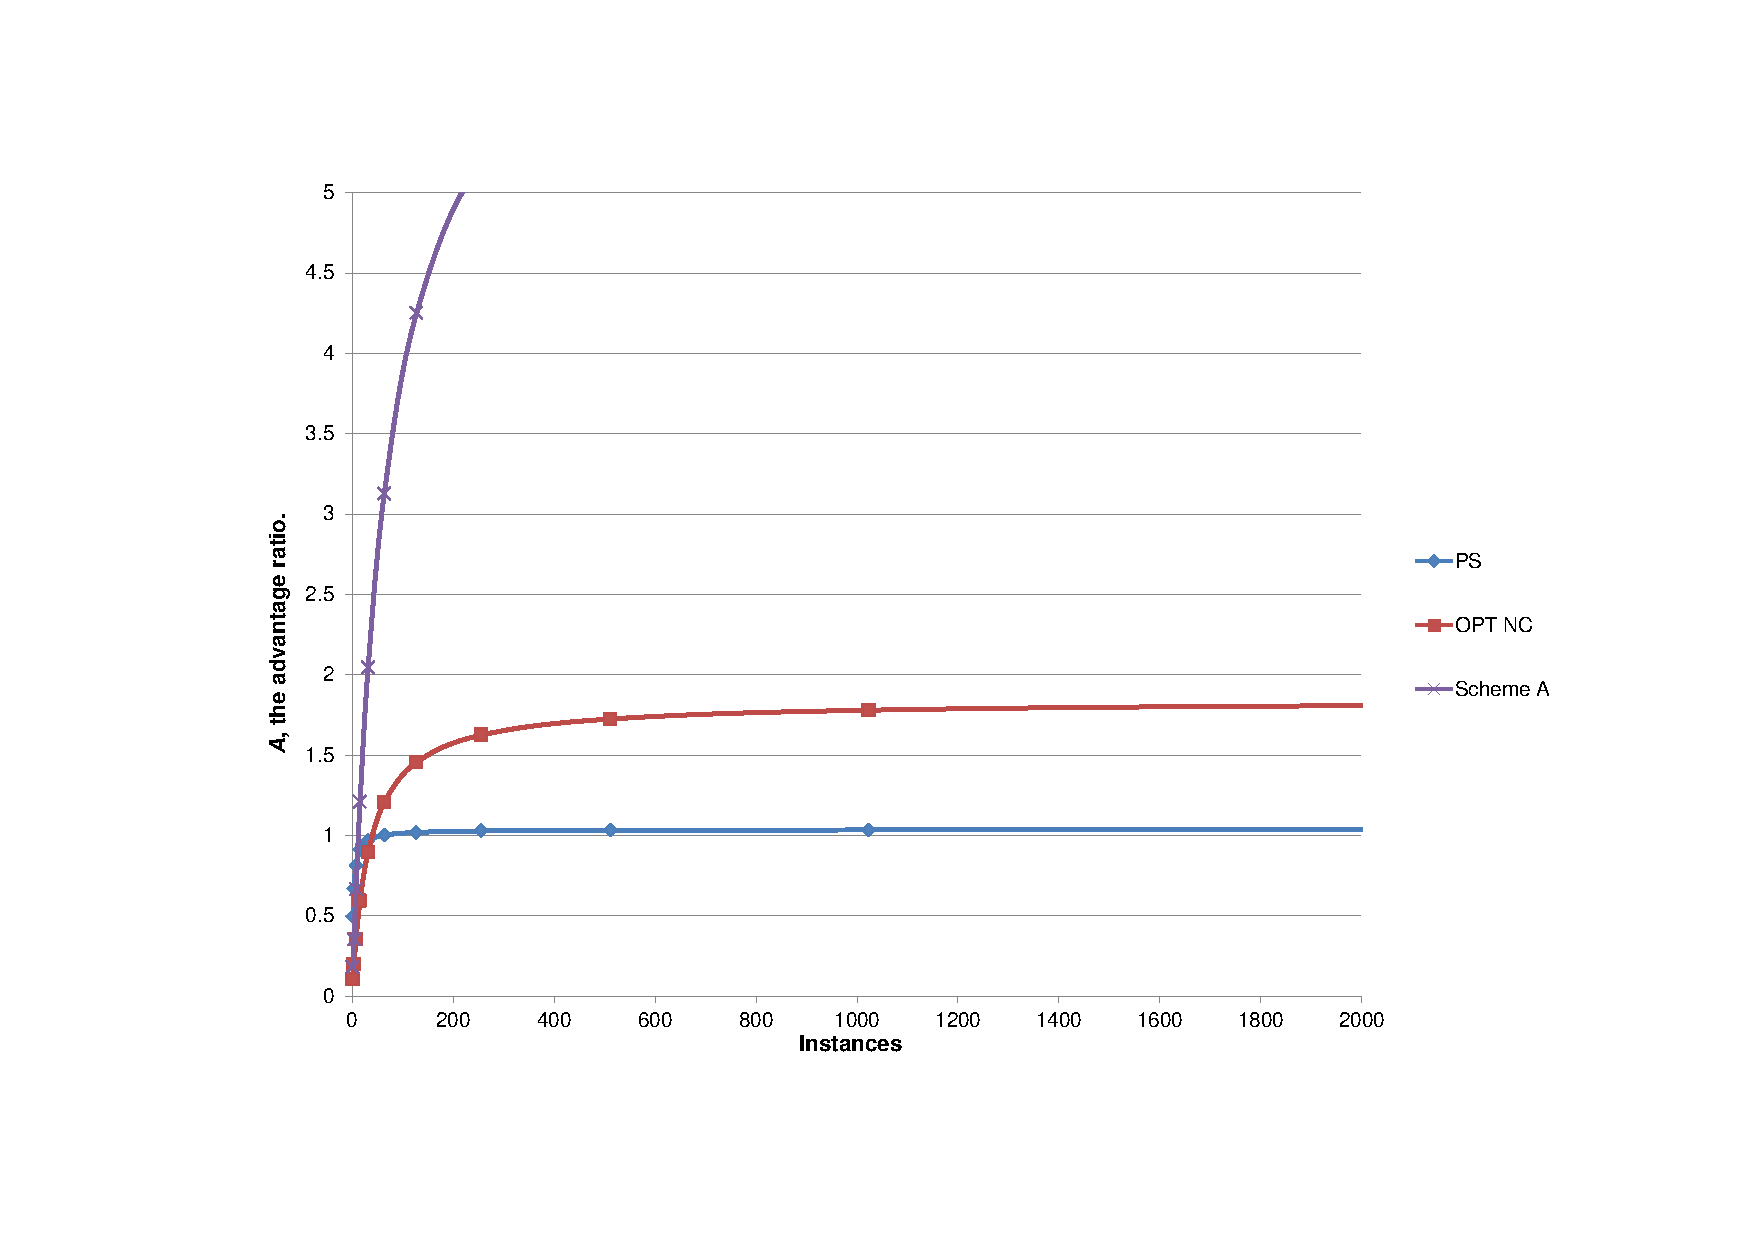
\includegraphics[scale=0.75, trim=5cm 3cm 0cm 4.5cm]{acpid-2.pdf} \label{acpid2}} \\
  \subfloat%[Part 2]
           {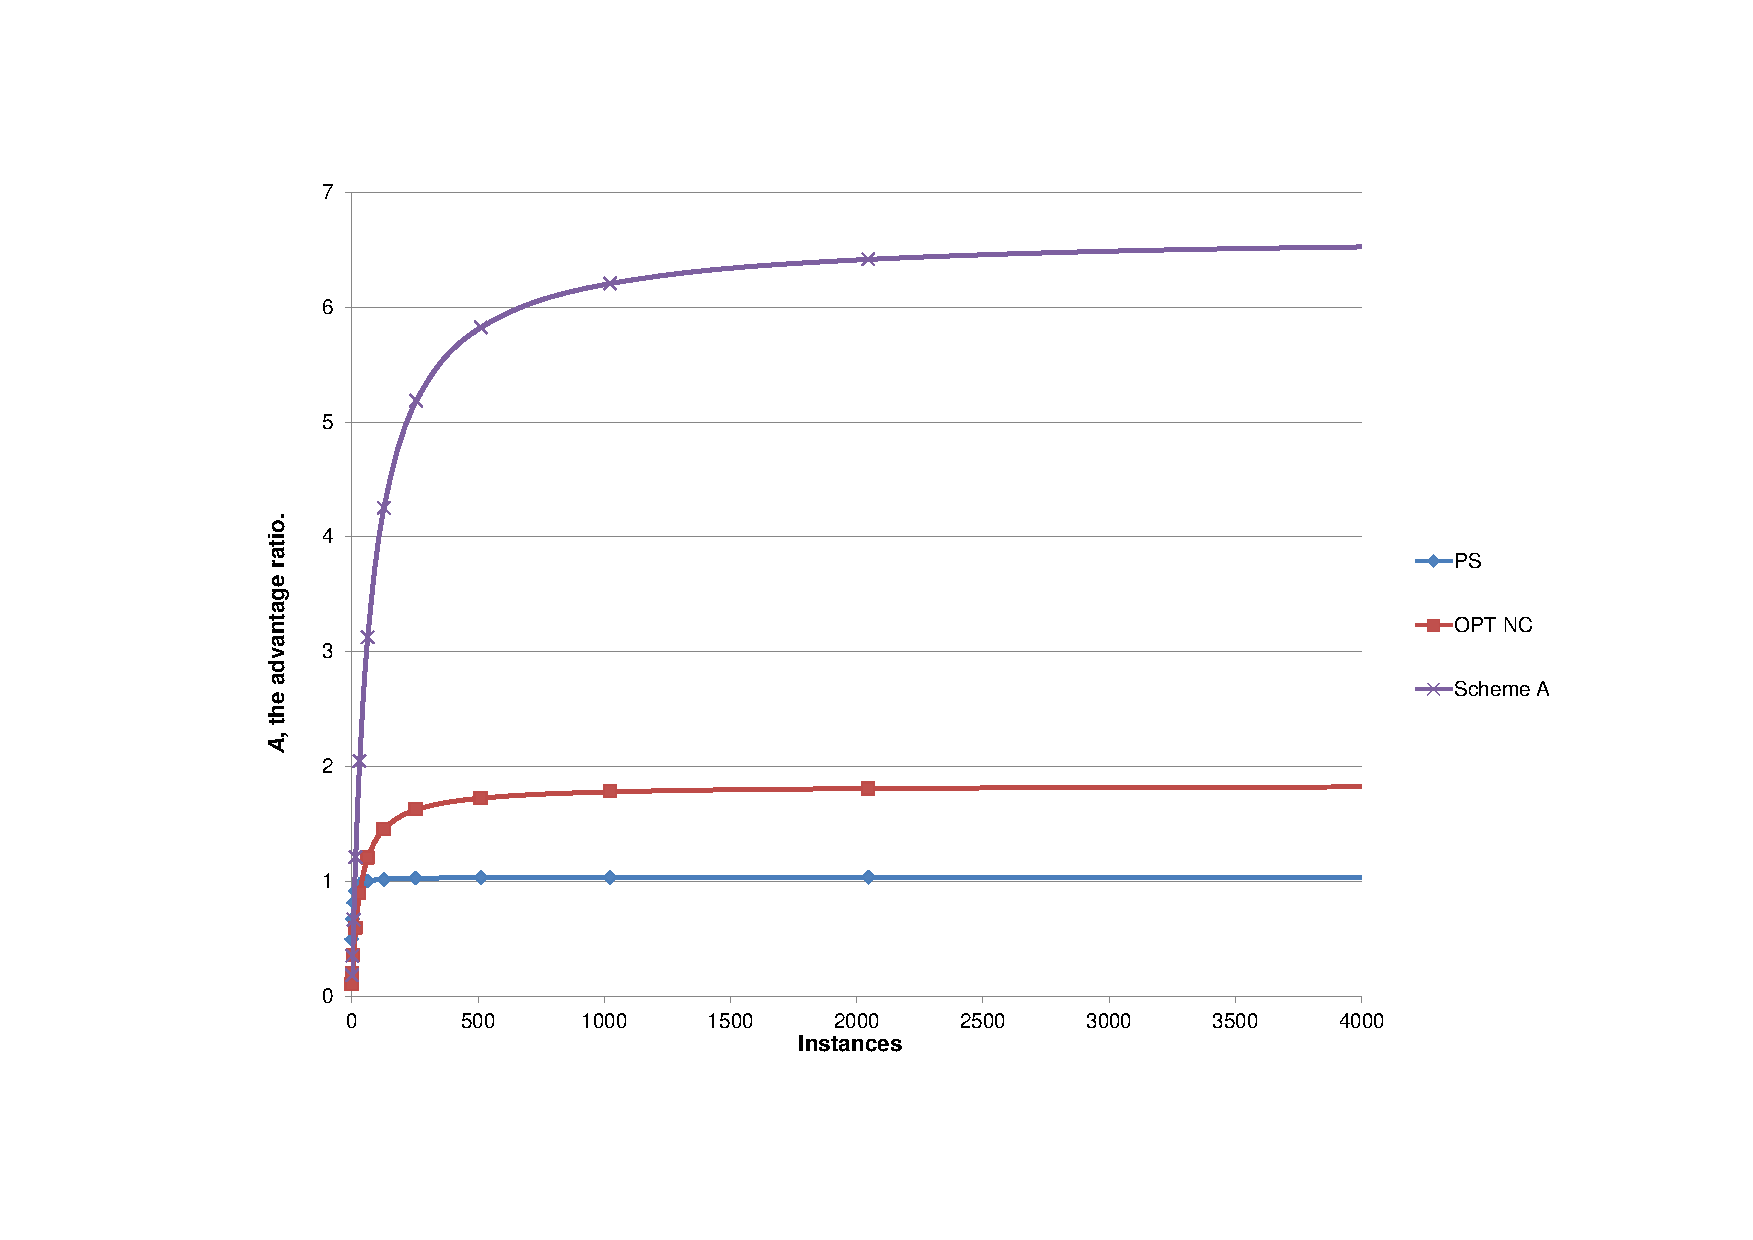
\includegraphics[scale=0.75, trim=5cm 3cm 0cm 3cm]{acpid-3.pdf} \label{acpid3}} 
  \caption[For \texttt{acpid}, $A$ as a function of $N$ (moderately conservative $\vec K$)]% 
          {For \texttt{acpid}, $A$ as a function of $N$ (moderately conservative $\vec K$).
          The top graph is a zoomed-in version of the lower graph.}
  \label{acpid23}
\end{figure}


\subsection{\texttt{anacron}}
\texttt{Anacron} is a user-space service
that complements \texttt{cron} by scheduling 
and executing tasks without requiring
the system to be continuously running.
Typically, \texttt{anacron} is used
to schedule daily, weekly or monthly
tasks for system-wide maintenance.

\begin{figure}[h]
  \center
  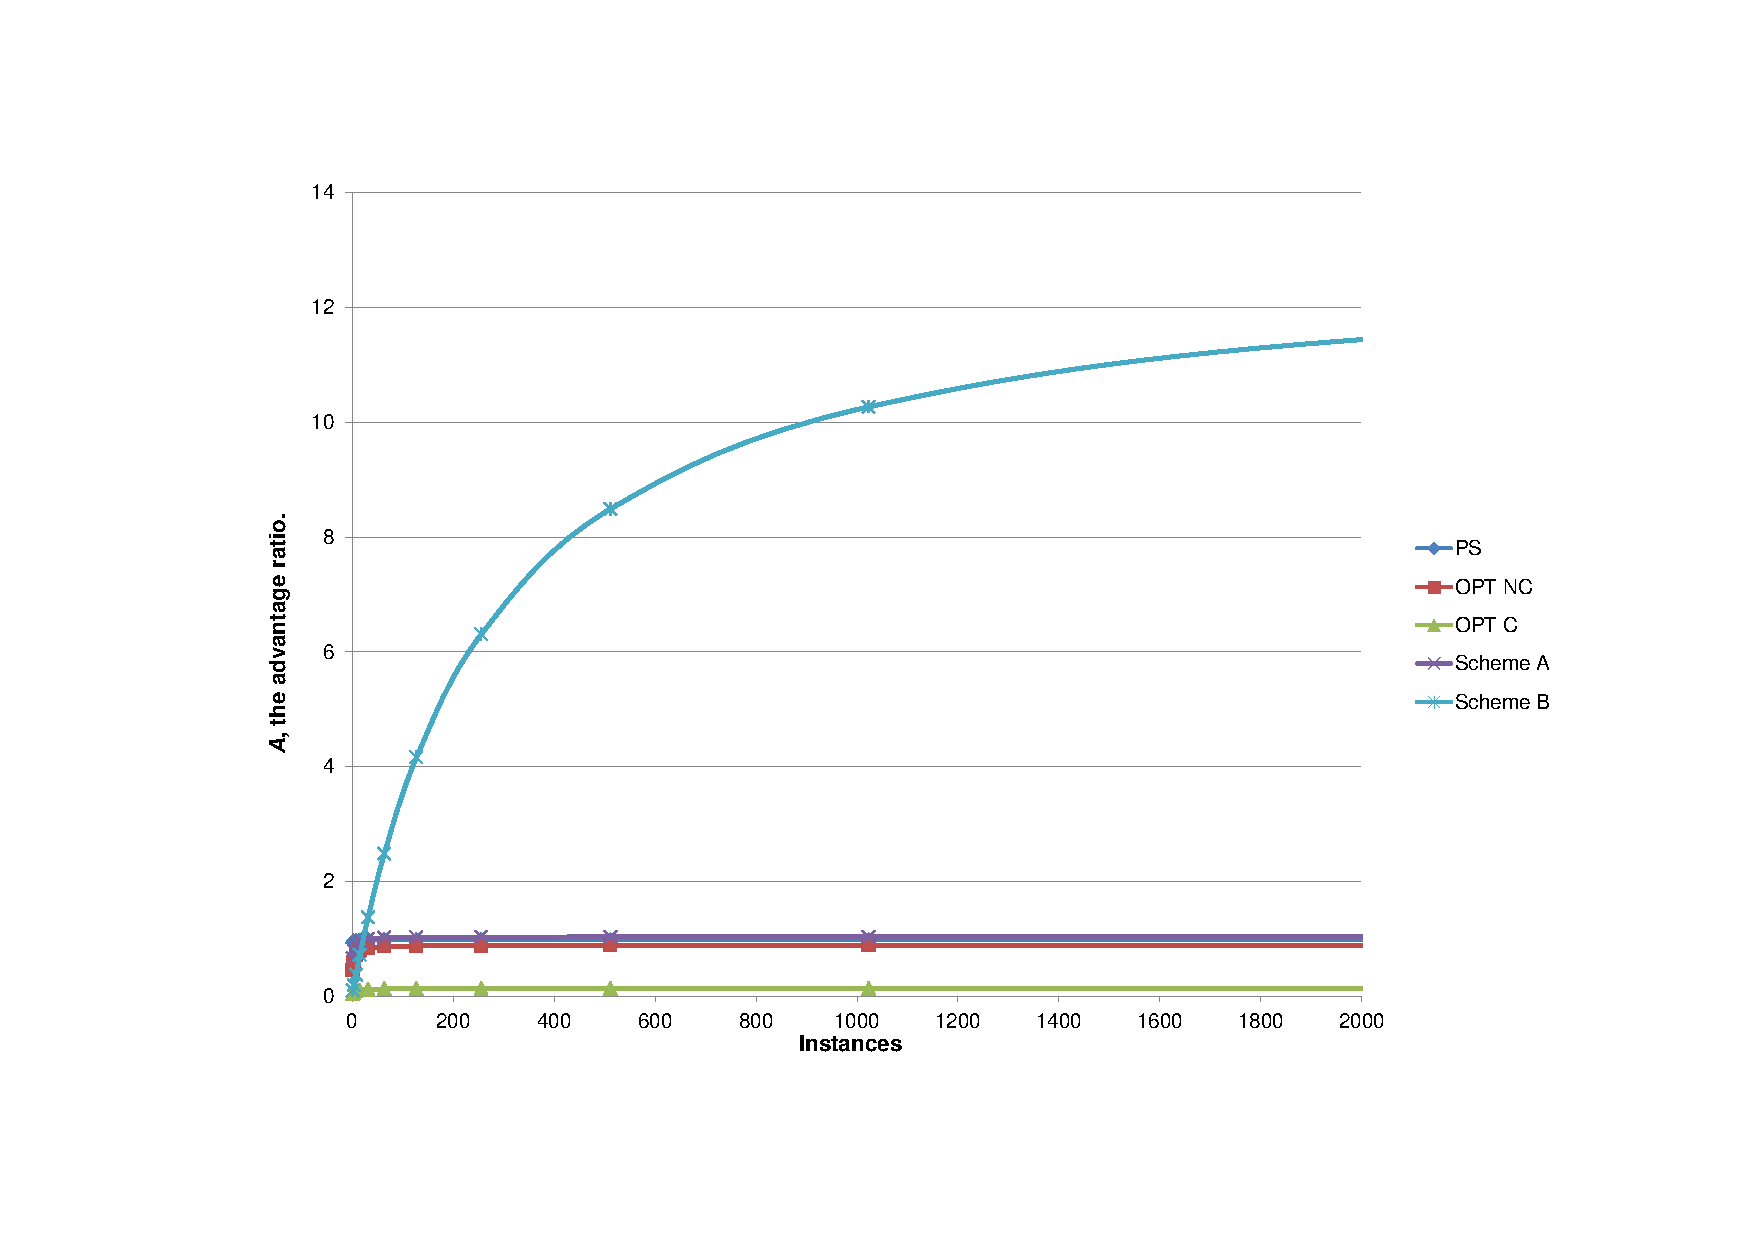
\includegraphics[scale=0.80, trim=5cm 3cm 0cm 3cm]{anacron-1.pdf}
  \caption[For \texttt{anacron}, $A$ as a function of $N$ (highly conservative $\vec K$)]% ]%
          {
            For \texttt{anacron}, computing $A$ as a function of $N$ (highly conservative $\vec K$).\newline
            \texttt{PS}, \texttt{OPT NC} and \texttt{OPT C} are lines for precise silhouetting, optimistic 
            silhouetting (excluding control flow) and optimistic silhouetting
            (including control flow) without any improvements; they
            serve as a baseline to measure the success of our techniques
            in our simulations. \texttt{Scheme A} and \texttt{Scheme B} represent the improved values of $A$
            achieved through deterministic silhouette execution:
            \texttt{Scheme A} reduces execution differences because
            of security, randomization and architecture-specific instructions;
            \texttt{Scheme B} incrementally adds the techniques used to
            virtualize the process ID layer on top of \texttt{Scheme A}.            
          }
  \label{anacron1}
\end{figure}

\newpage
\noindent Figure \ref{anacron1} shows the results of our experiments
to measure any improvements in $A$ from the techniques described in Section \ref{silimprove}.
Our workload consisted of simple boot-time initialization of \texttt{anacron}
for the case when \texttt{cron.weekly} tasks need to be executed.

\texttt{Scheme A} includes the techniques we described to reduce
execution differences that arise from randomization, security and time.
\texttt{Scheme B} adds {\em process ID virtualization}
to \texttt{Scheme A}; \texttt{anacron} interacts
frequently with process IDs because it uses them to track
child jobs spawned. \texttt{Scheme B} is sufficient to eliminate active fork-points in \texttt{anacron}
entirely. Thus, \texttt{Scheme B} uses precise silhouetting
in which execution does not diverge till the very end of our workload,
whereas \texttt{Scheme A} elongates the execution prefix ($P$) slightly
to 5.50\%. As before, \texttt{Scheme A} and \texttt{Scheme B} simulate {\em write compression}
to improve $A$. 

As shown in Figure \ref{anacron1}, \texttt{Scheme A}
does not affect $A$ much; because of the small increase
in $P$ (the prefix), $A$ remains close to 1.
However, \texttt{Scheme B} improves the ratio $A$ and
takes it to a reasonably high value ($A > 10$), converting a CPU load {\em increase}
into a CPU load reduction. $A$ scales better as $N$ increases for \texttt{anacron}
than for \texttt{acpid}, because \texttt{anacron} has 
a $10\times$ lower memory-writes-to-instructions (i.e. $M/I$) ratio 
than \texttt{acpid}; this means there is less 
overhead when silhouettes restore the leader's memory image 
in \texttt{anacron}.  Eventually, however, the 
very conservative design overhead $\vec K$
causes $A$ to plateau when $N$ becomes very large.

As before, Figure \ref{anacron2} shows how $A$ changes with $N$ when we pick less conservative
values of overhead constants ($\vec K$). The achieved values of $A$ 
exceed 50 for $N < 3000$, a significant simulated reduction in the CPU
pressure from user-space. The value of $A$ scales well for moderately high $N$
(Figure \ref{anacron2}) before it plateaus due
to expected design overhead.

The highest theoretically possible
$A$ ($A_{MAX}$) is equal to $\frac{I}{F+M}$. For our samples of \texttt{anacron}, $A_{MAX}$ 
is about 377, and we again get within a factor of 10 of that number in Figure \ref{acpid3}. 

\begin{figure}
  \centering
  \subfloat%[Part 1]
           {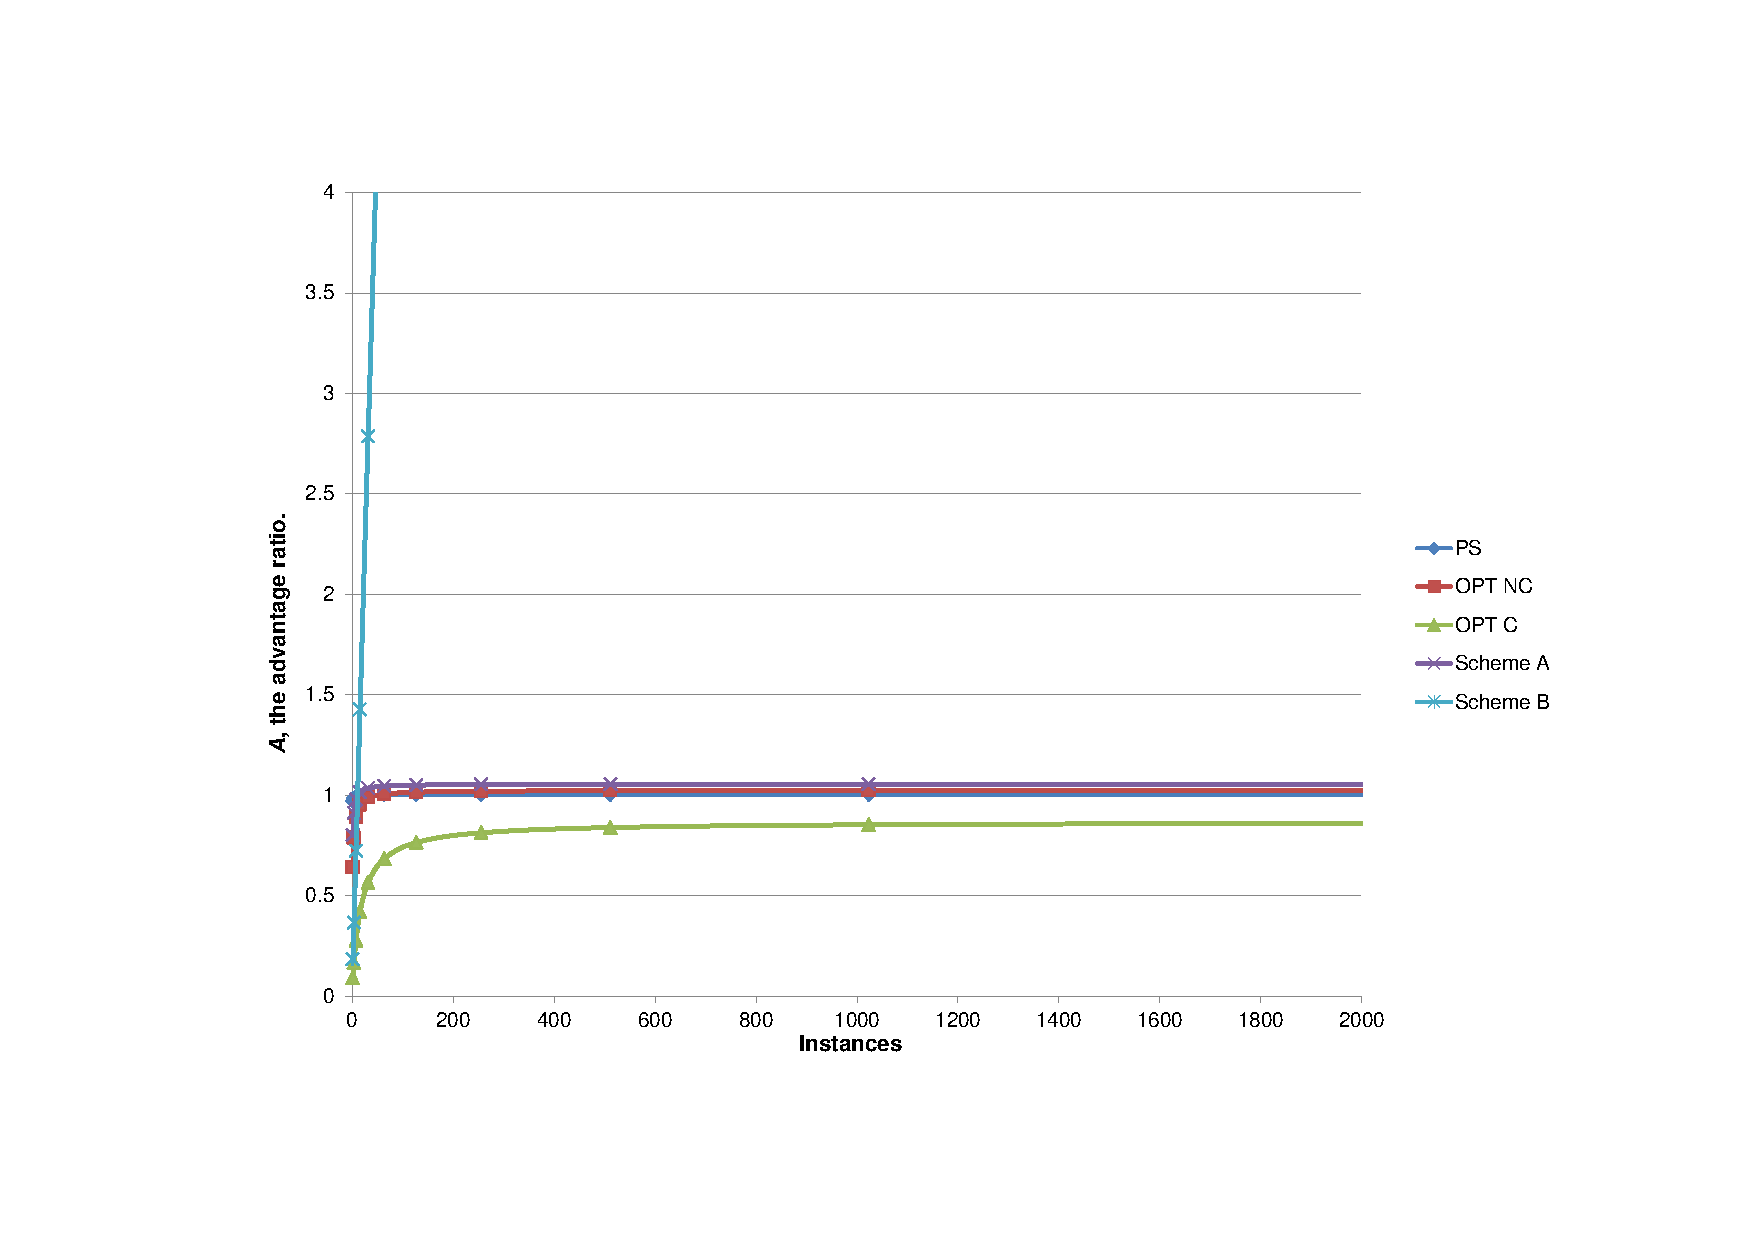
\includegraphics[scale=0.75, trim=5cm 3cm 0cm 4.5cm]{anacron-2.pdf} \label{anacron2}} \\
  \subfloat%[Part 2]
           {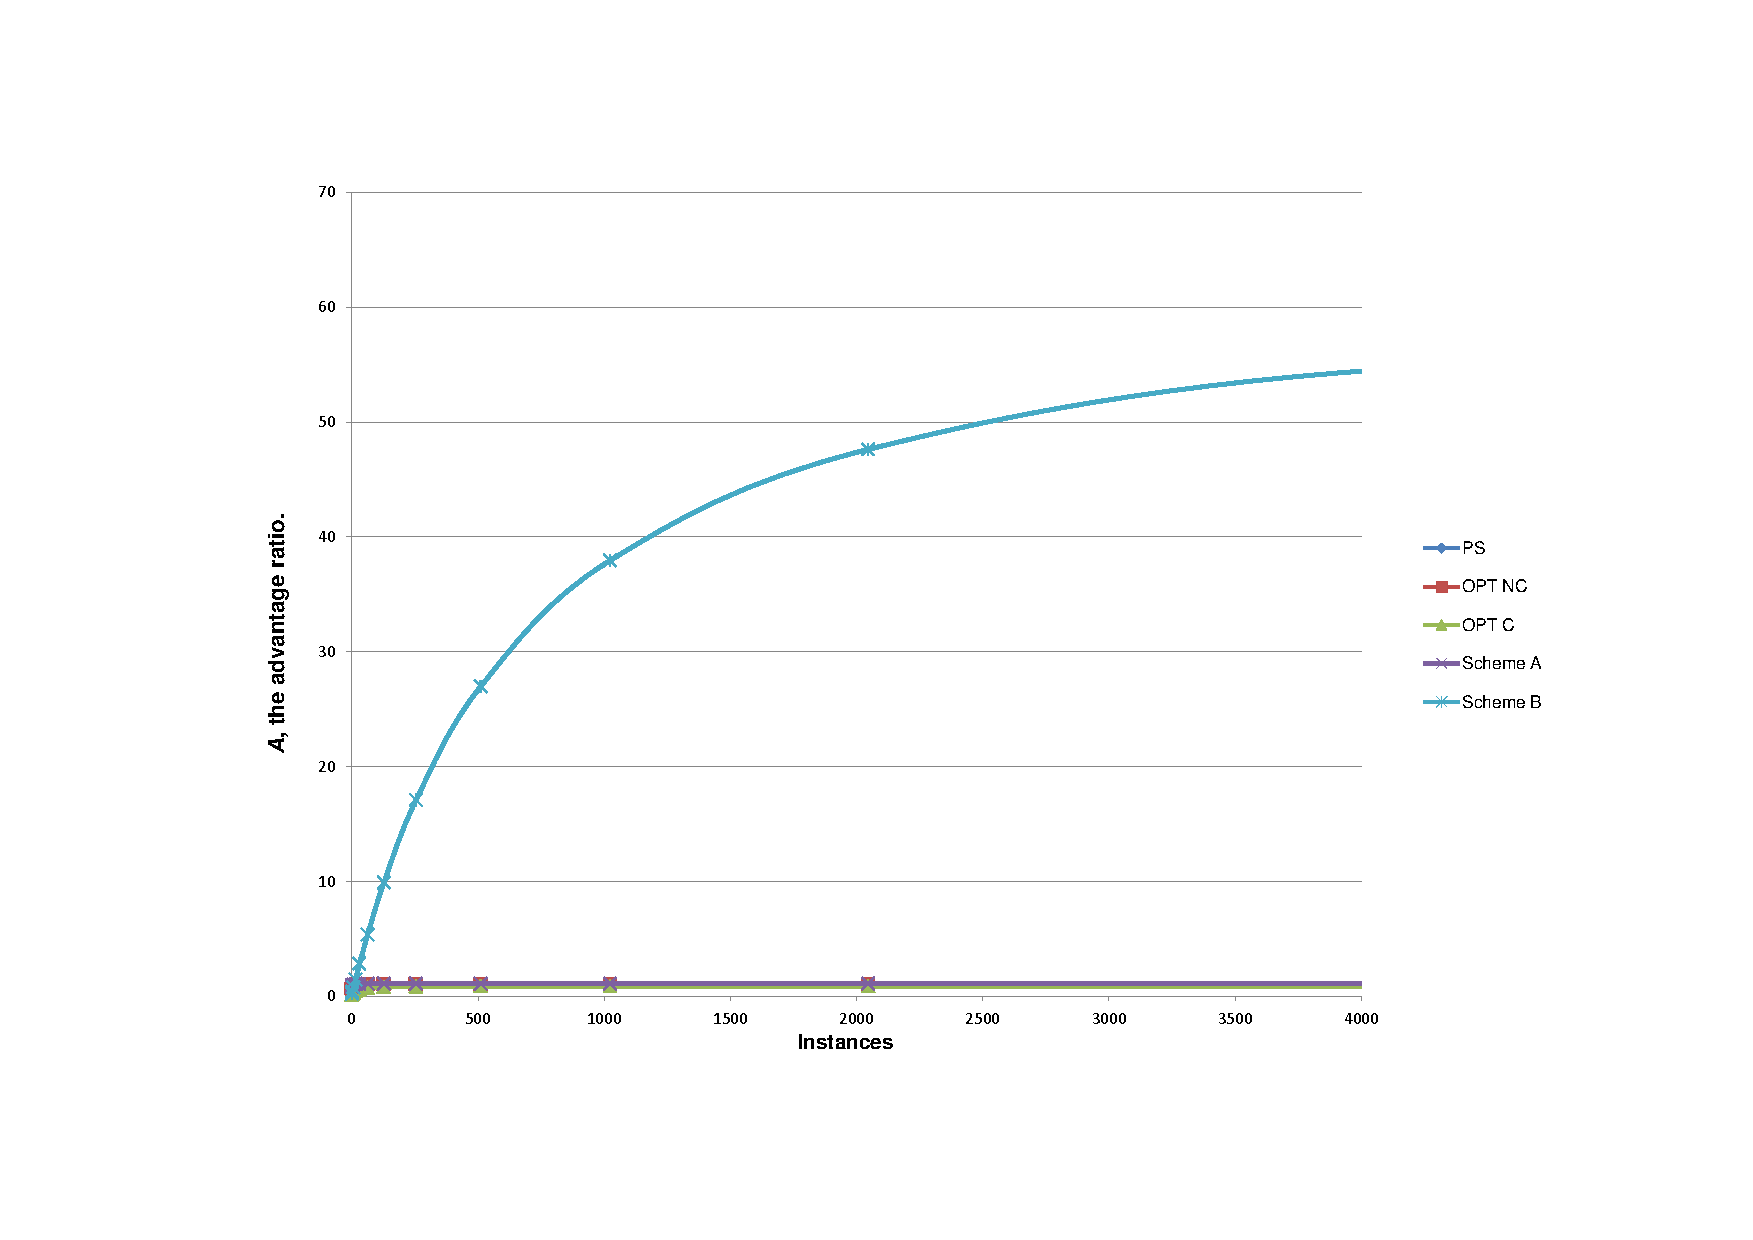
\includegraphics[scale=0.75, trim=5cm 3cm 0cm 3cm]{anacron-3.pdf} \label{anacron3}} 
  \caption[For \texttt{anacron}, $A$ as a function of $N$ (moderately conservative $\vec K$)]% 
          {For \texttt{anacron}, $A$ as a function of $N$ (moderately conservative $\vec K$).
          The top graph is a zoomed-in version of the lower graph.}
  \label{anacron23}
\end{figure}


\subsection{\texttt{cron}}
The program {\texttt{cron}} is a job scheduler
that allows users to periodically execute scripts or programs;
it automates system maintenance or administration
and complements \texttt{anacron}. \texttt{Cron}
assumes that the system is running continuously; 
\texttt{anacron} catches jobs missed
by \texttt{cron} while the computer is turned off.

\begin{figure}[h]
  \center
  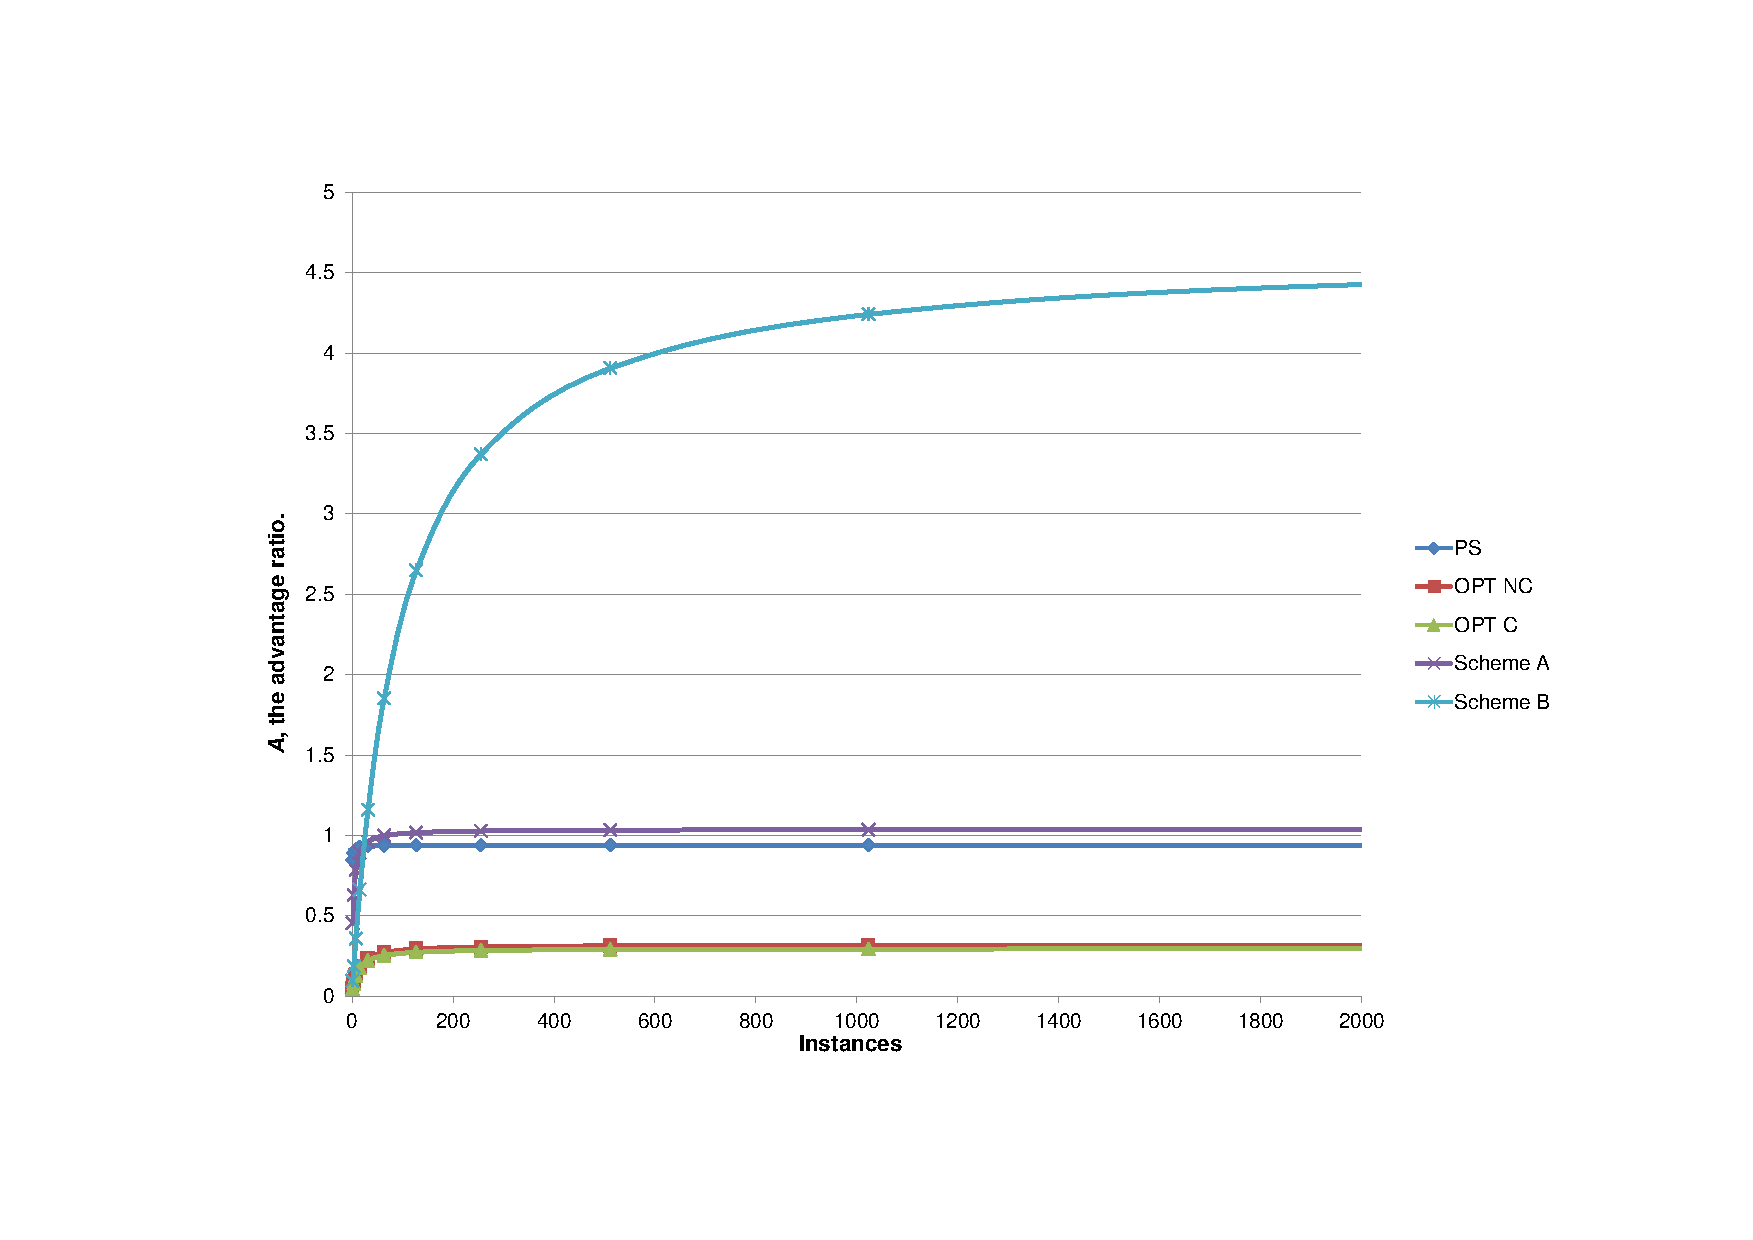
\includegraphics[scale=0.80, trim=5cm 3cm 0cm 3cm]{cron-1.pdf}
  \caption[For \texttt{cron}, $A$ as a function of $N$ (highly conservative $\vec K$)]% ]%
          {
            For \texttt{cron}, computing $A$ as a function of $N$ (highly conservative $\vec K$).\newline
            \texttt{PS}, \texttt{OPT NC} and \texttt{OPT C} are lines for precise silhouetting, optimistic 
            silhouetting (excluding control flow) and optimistic silhouetting
            (including control flow) without any improvements; they
            serve as a baseline to measure the success of our techniques
            in our simulations. \texttt{Scheme A} and \texttt{Scheme B} represent the improved values of $A$
            achieved through deterministic silhouette execution:
            \texttt{Scheme A} reduces execution differences because
            of security, randomization and architecture-specific instructions;
            \texttt{Scheme B} incrementally adds the techniques used to
            virtualize the process ID layer on top of \texttt{Scheme A}.            
          }
  \label{cron1}
\end{figure}

\newpage
\noindent Figure \ref {cron1} shows the results of our experiments
to measure any improvements in $A$ from the techniques described in Section \ref{silimprove}.
Our workload consisted of a few iterations of the main loop in \texttt{cron}.
The analysis for \texttt{cron} is somewhat similar to that of 
\texttt{anacron} because of the similar nature of the two programs.

As before, \texttt{Scheme A} includes the techniques we described to reduce
execution differences that arise from randomization, security and time.
Just like \texttt{anacron}, \texttt{cron} uses process IDs
in its interactions with any spawned child jobs,
so \texttt{Scheme A} itself is not effective and only elongates the 
execution prefix ($P$) to 12.40\%.
However, \texttt{Scheme B} adds {\em process ID virtualization} to
\texttt{Scheme A}, which is sufficient to eliminate
execution differences in \texttt{cron}.
{Scheme B} thus uses precise silhouetting
in which execution does not branch till the very end of our workload.
Both schemes simulate {\em write compression}.

As shown in Figure \ref{cron1}, \texttt{Scheme B} improves $A$ 
to be slightly higher than 1. In fact, $A > 4$, which represents                                                                                             
a theoretical reduction in CPU pressure unlike the baseline
scores. However, the achieved $A$ is much lower for \texttt{cron} than that for \texttt{anacron},
which is probably because of the lower memory-writes-to-instructions (i.e. $M/I$) ratio
for the latter.

Figure \ref{cron23} shows how $A$ changes with $N$ when we pick less conservative
values of overhead constants ($\vec K$) 
The achieved values of $A$ 
exceed 17 for $N < 1000$, which represents a significant
theoretical reduction in the number of user-space instructions
executed. The value of $A$ scales well for small $N$
(Figure \ref{cron2}) but plateaus as expected
for very large $N$.

The highest theoretically possible
$A$, $A_{MAX} = \frac{I}{F+M}$  is about 120, and we get within a factor of 10 of that number in Figure \ref{cron3}. 

\begin{figure}
  \centering
  \subfloat%[Part 1]
           {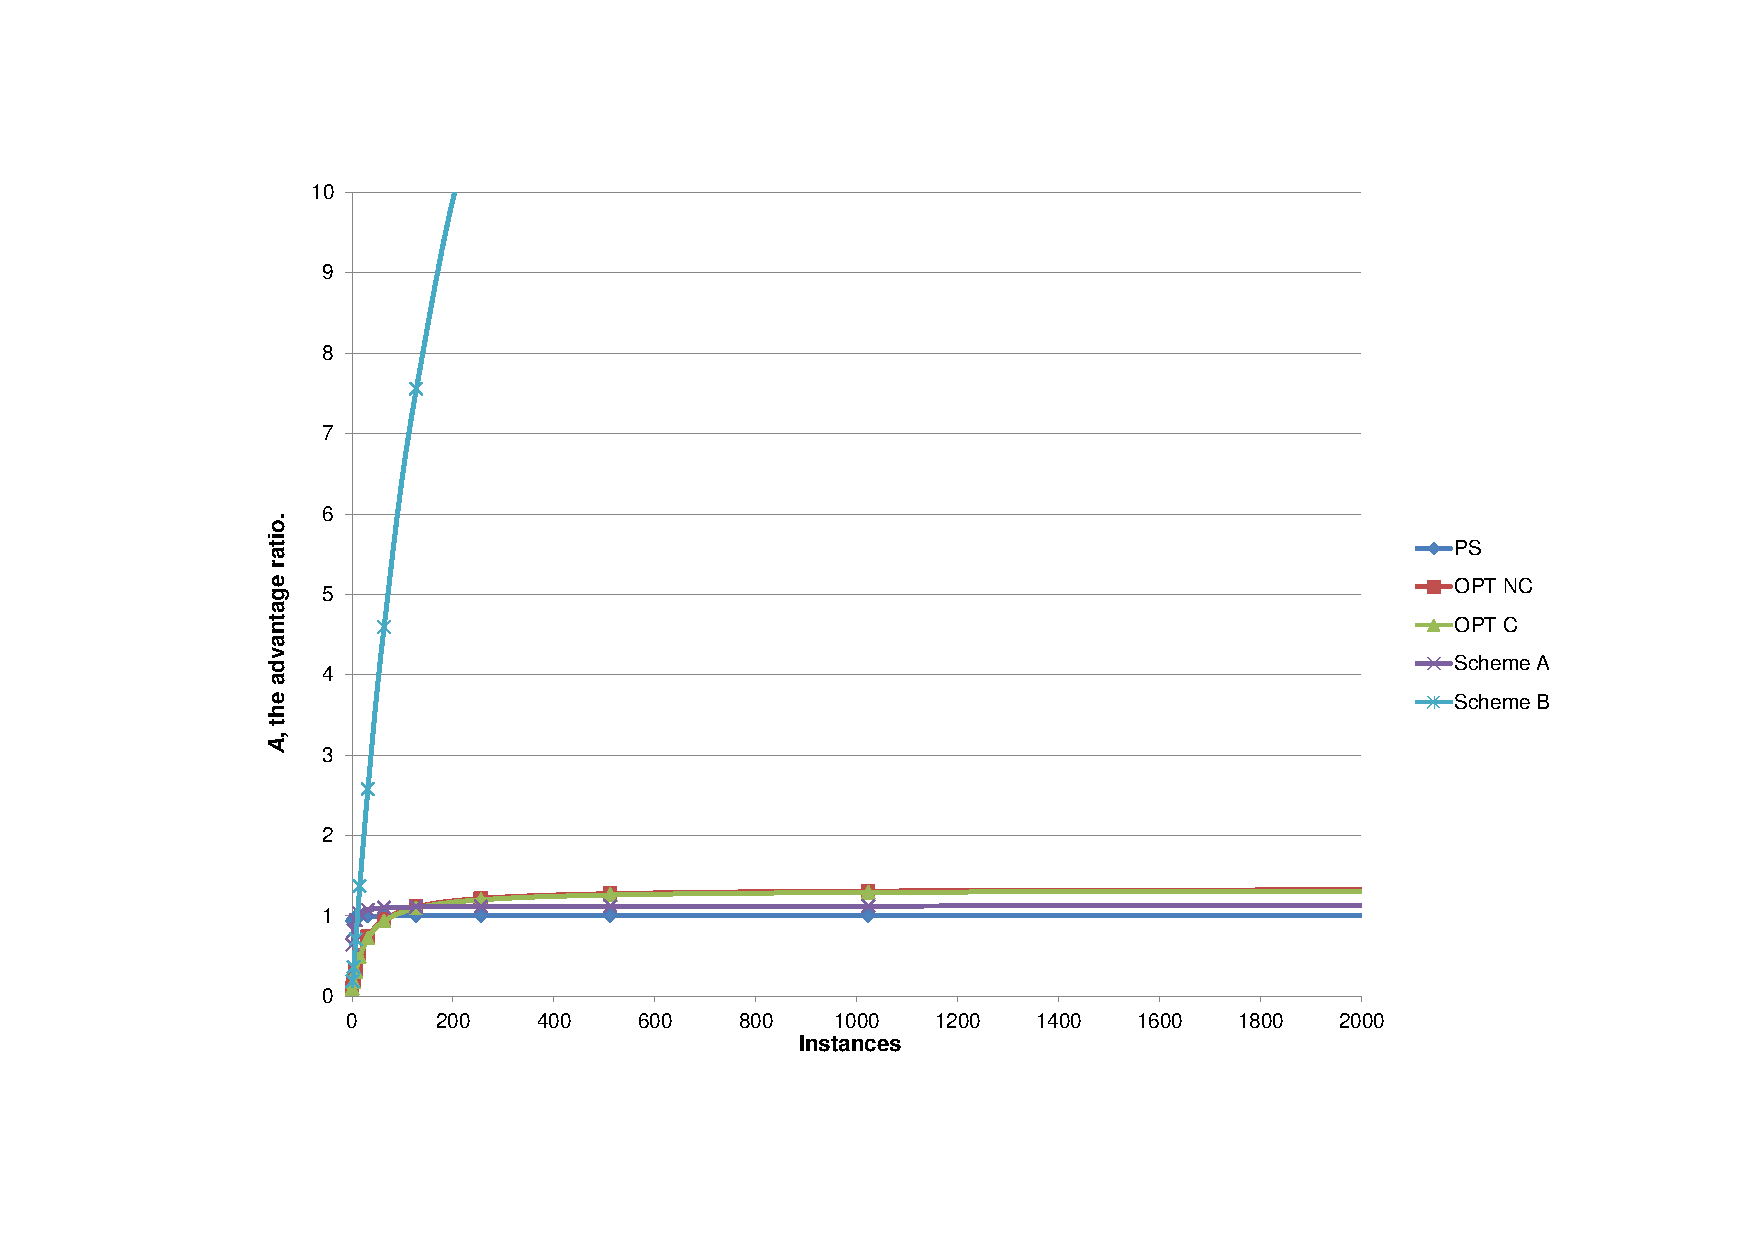
\includegraphics[scale=0.75, trim=5cm 3cm 0cm 4.5cm]{cron-2.pdf} \label{cron2}} \\
  \subfloat%[Part 2]
           {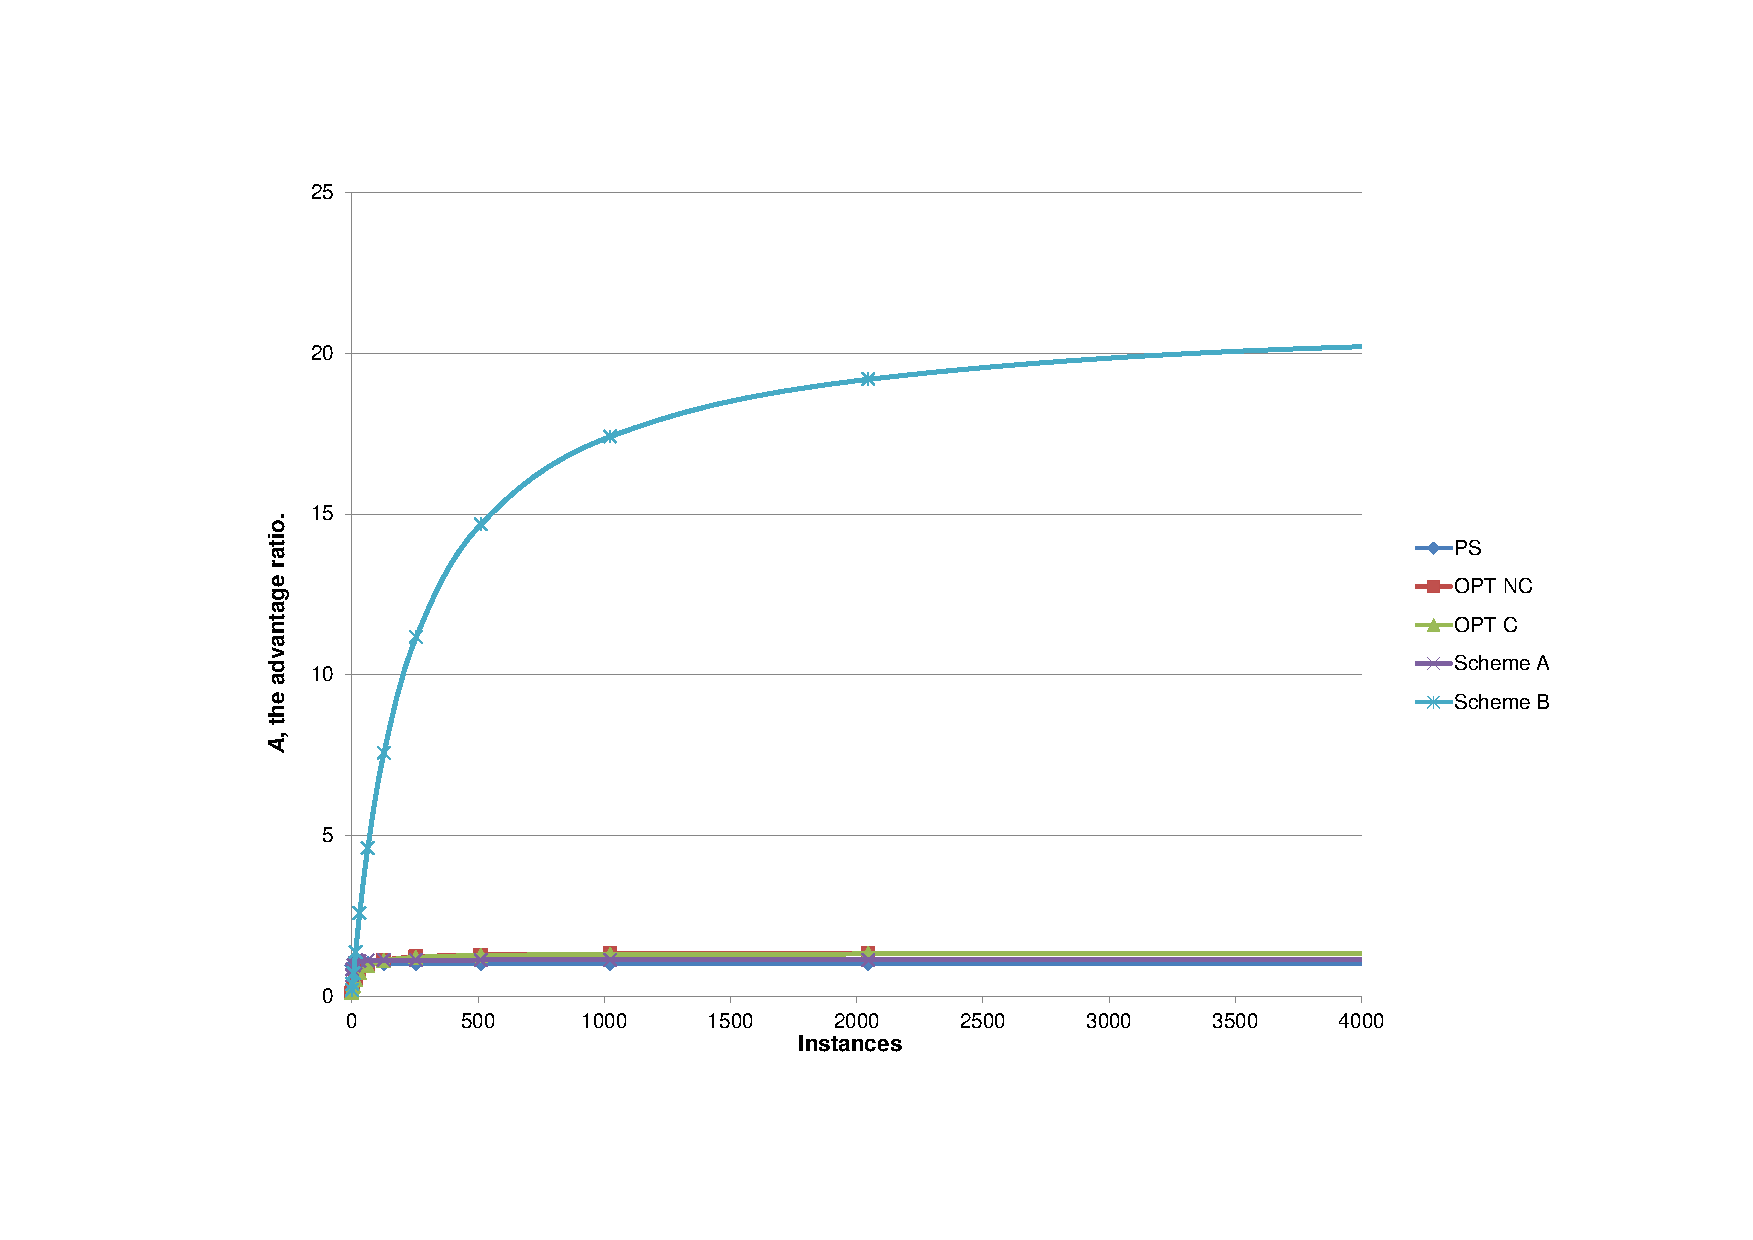
\includegraphics[scale=0.75, trim=5cm 3cm 0cm 3cm]{cron-3.pdf} \label{cron3}} 
  \caption[For \texttt{cron}, $A$ as a function of $N$ (moderately conservative $\vec K$)]% 
          {For \texttt{cron}, $A$ as a function of $N$ (moderately conservative $\vec K$).
          The top graph is a zoomed-in version of the lower graph.}
  \label{cron23}
\end{figure}

\newpage
\subsection{\texttt{cups}} \label{cups:hard}
The \texttt{cups} program is a printing service
for Linux systems that allows a computer to act as a print server. 
Because of the modularity in \texttt{cups}, the print {\em scheduler}
can easily communicate with many kinds of printers (including local, remote or
virtual printers).

\begin{figure}[h]
  \center
  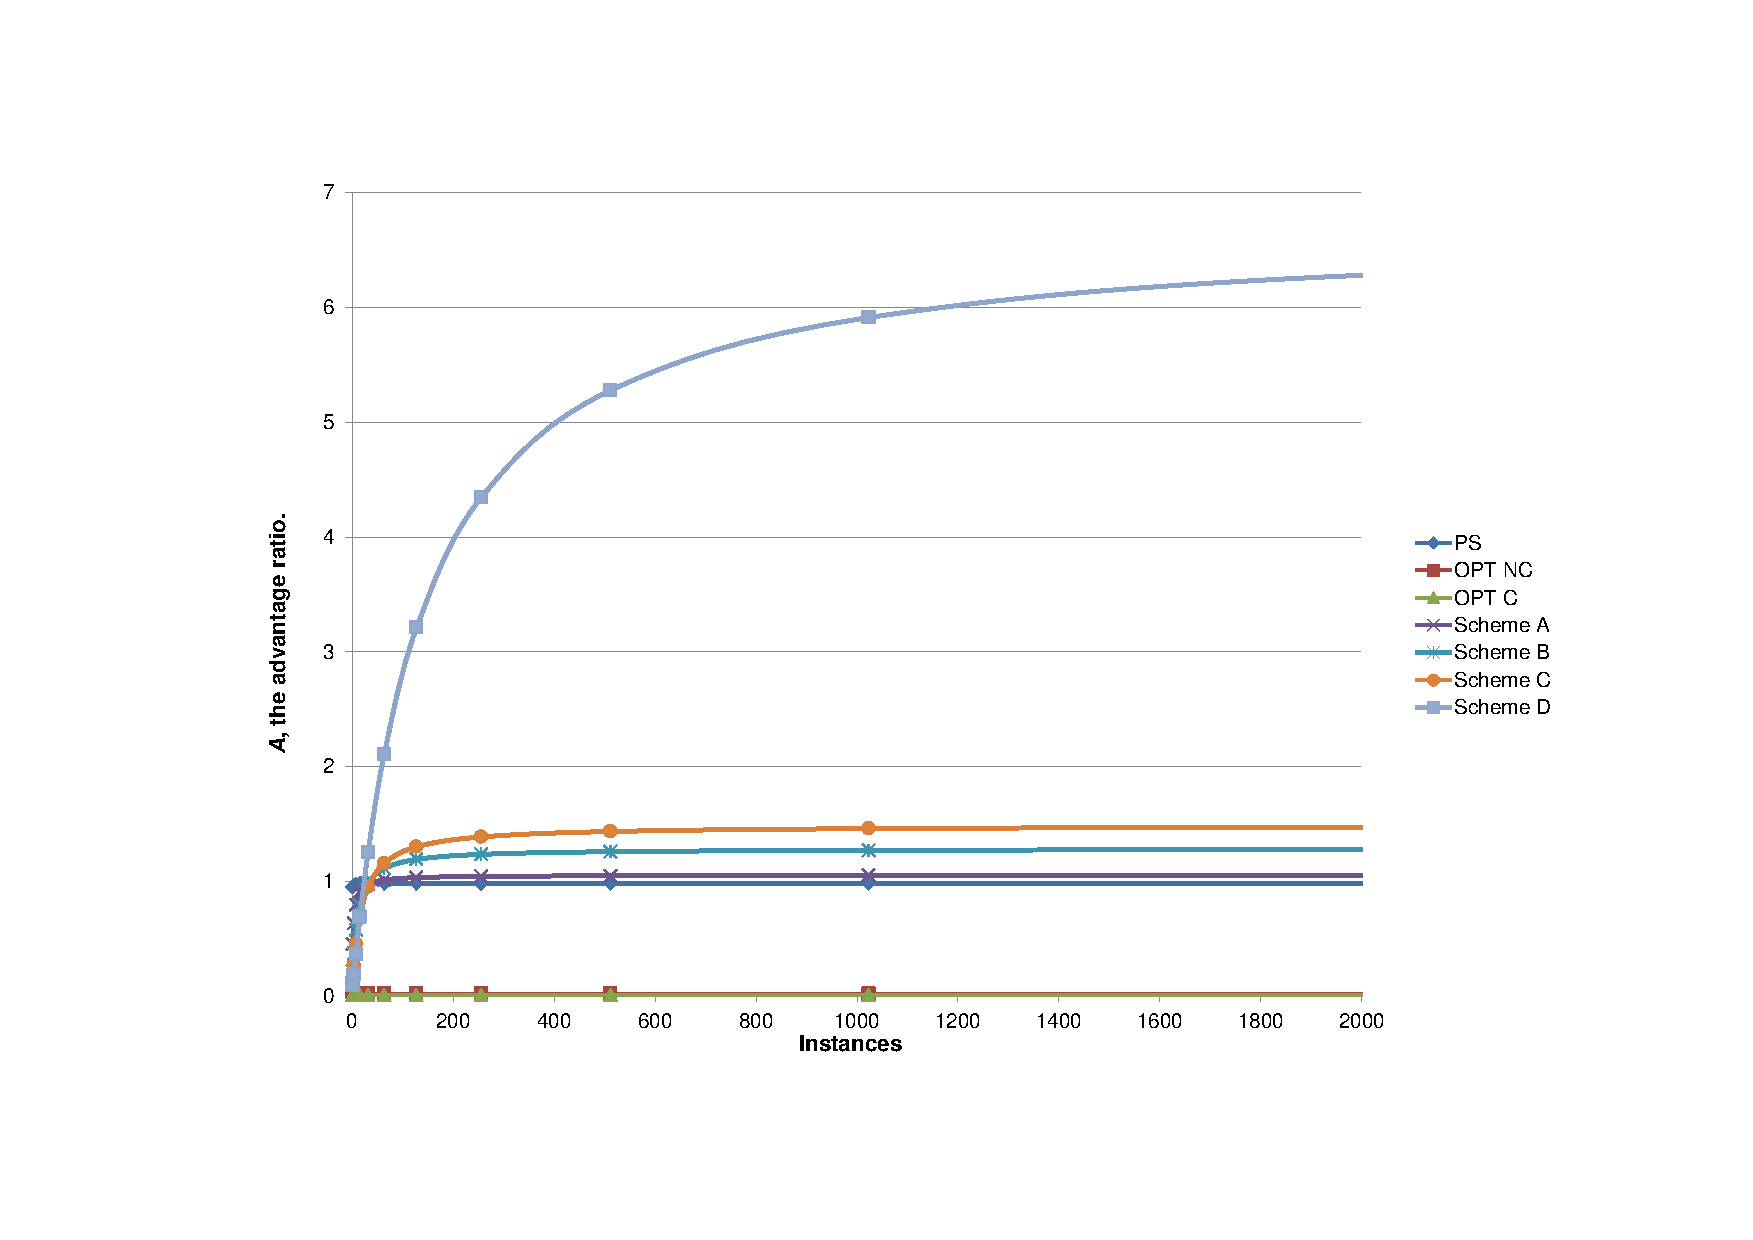
\includegraphics[scale=0.80, trim=5cm 3cm 0cm 3cm]{cups-1.pdf}
  \caption[For \texttt{cups}, $A$ as a function of $N$ (highly conservative $\vec K$)]% ]%
          {
            For \texttt{cups}, computing $A$ as a function of $N$ (highly conservative $\vec K$).\newline
            \texttt{PS}, \texttt{OPT NC} and \texttt{OPT C} are lines for precise silhouetting, optimistic 
            silhouetting (excluding control flow) and optimistic silhouetting
            (including control flow) without any improvements; they
            serve as a baseline to measure the success of our techniques
            in our simulations. \texttt{Scheme A}, \texttt{Scheme B}, \texttt{Scheme C} and
            \texttt{Scheme D} represent the improved values of $A$
            achieved through incremental levels of deterministic silhouette execution.
          }
  \label{cups1}
\end{figure}

\newpage
Figure \ref{cups1} shows how $A$ depends on $N$ for various design
strategies for silhouette execution in \texttt{cups}. The workload
considered was a few iterations of the \texttt{cups} daemon on a 
machine configured to print remotely to \texttt{cups.csail.mit.edu}.
The various schemes illustrated in Figure \ref{cups1} are:
\begin{itemize}
\item {\bf Scheme A} \newline
  This scheme reduces execution differences that occur because of Linux security
  features, time, randomization and architecture-specific instructions.
\item {\bf Scheme B} \newline
  This scheme includes Scheme A, and also handles execution
  differences from \texttt{Netlink} and the process ID layer
  in Linux.
\item {\bf Scheme C} \newline
  This scheme includes Scheme B, and also handles execution
  differences from file contents (e.g. cache files)
  or file timestamps (e.g. from \texttt{stat}).
  Scheme $C$ reduces fork-points from \texttt{stat}
  calls by tainting their timestamps automatically
  and deletes/forces agreements between cache
  files if they do not matter for correctness.

\item {\bf Scheme D} \newline
  This scheme includes Scheme C, and also handles execution
  differences from variable timing,
  latency or ordering of I/O operations e.g.
  signals or scalable polling (\texttt{epoll})
  engines.
\end{itemize}
For each of these schemes, the measured advantage ratio
is higher than 1, so they all successfully reduce CPU
pressure in our simulations unlike the baseline designs.
\texttt{Scheme D} is necessary because \texttt{cups}
uses signals and \texttt{epoll}; using it,
the achieved value of $A$ is reasonably high ($A > 15$
for $N < 500$). \texttt{Scheme D} eliminates
all active fork-points, so we can
use precise silhouetting 
for \texttt{cups}. 

\begin{figure}
  \centering
  \subfloat%[Part 1]
           {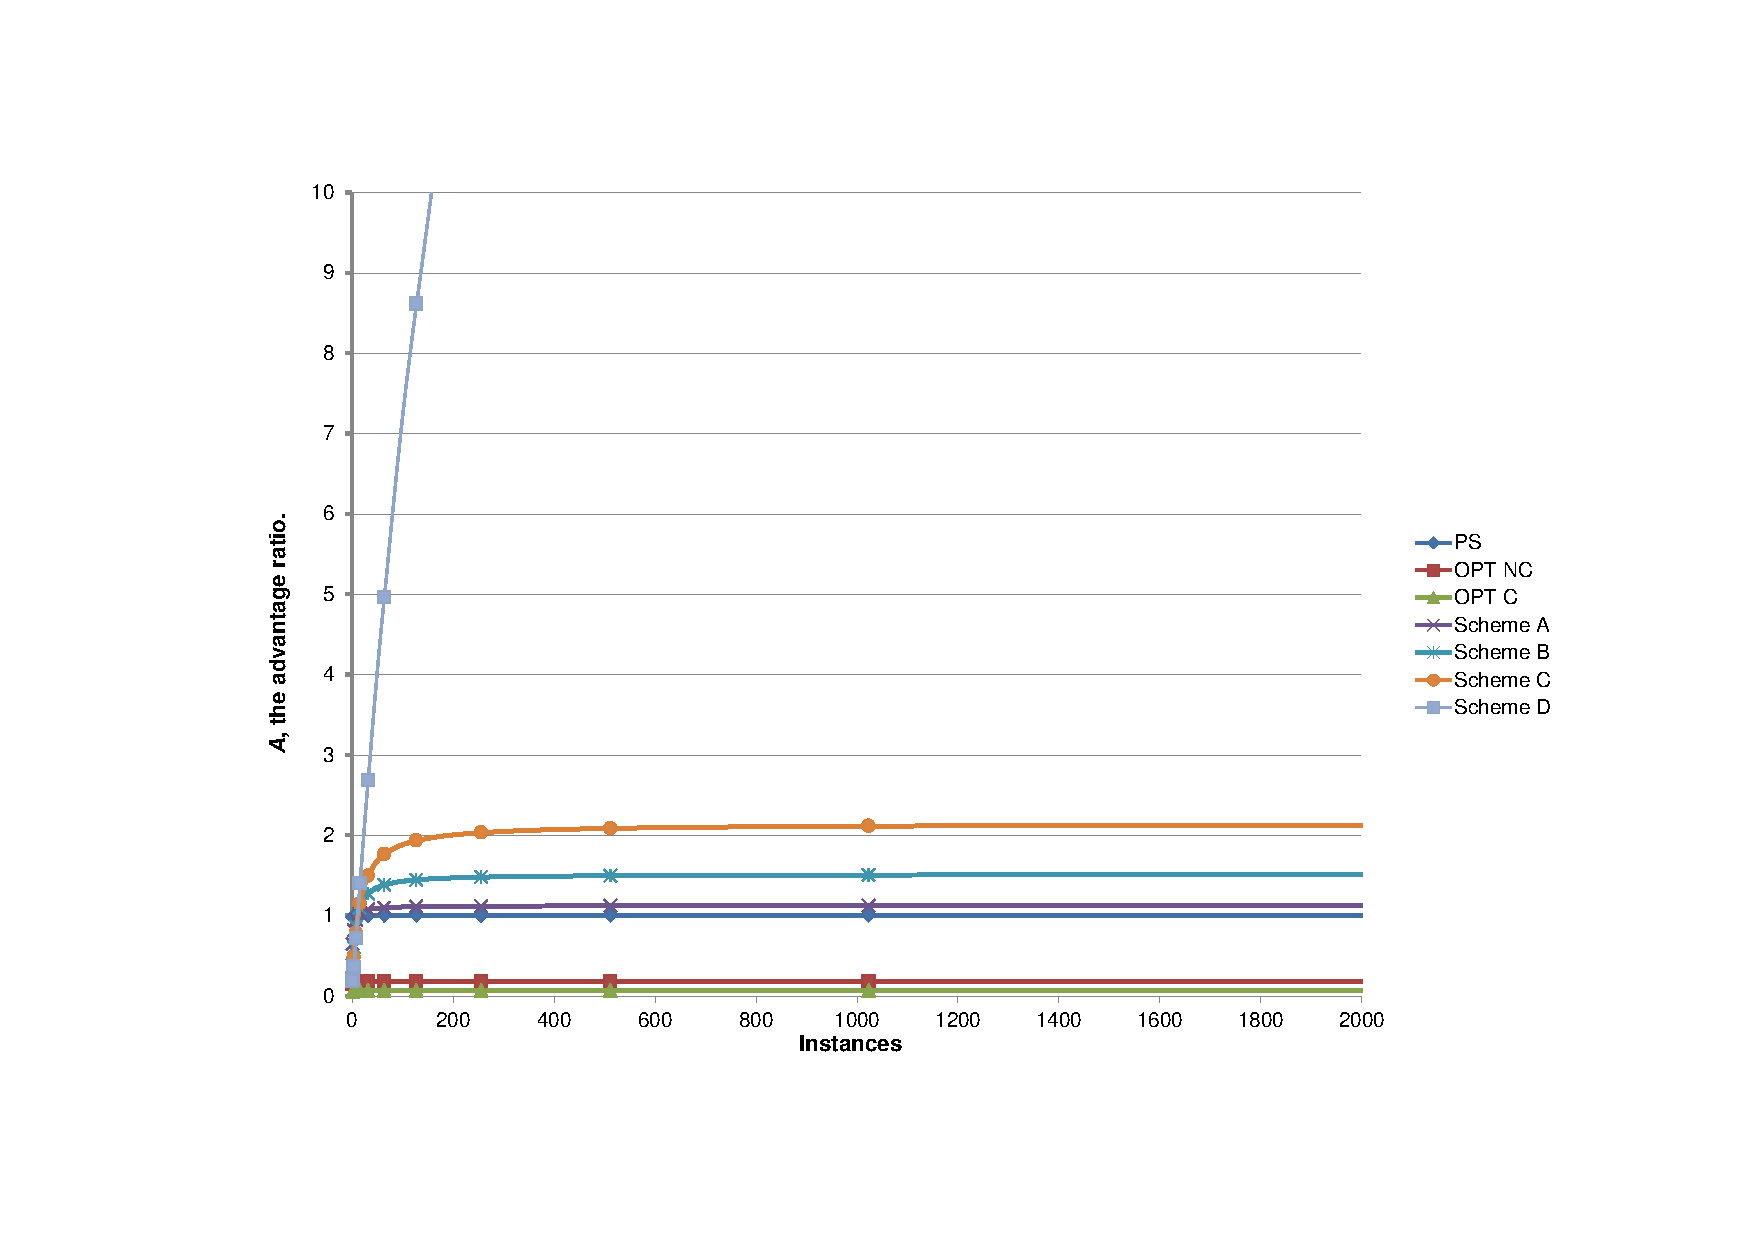
\includegraphics[scale=0.75, trim=5cm 3cm 0cm 4.5cm]{cups-2.pdf} \label{cups2}} \\
  \subfloat%[Part 2]
           {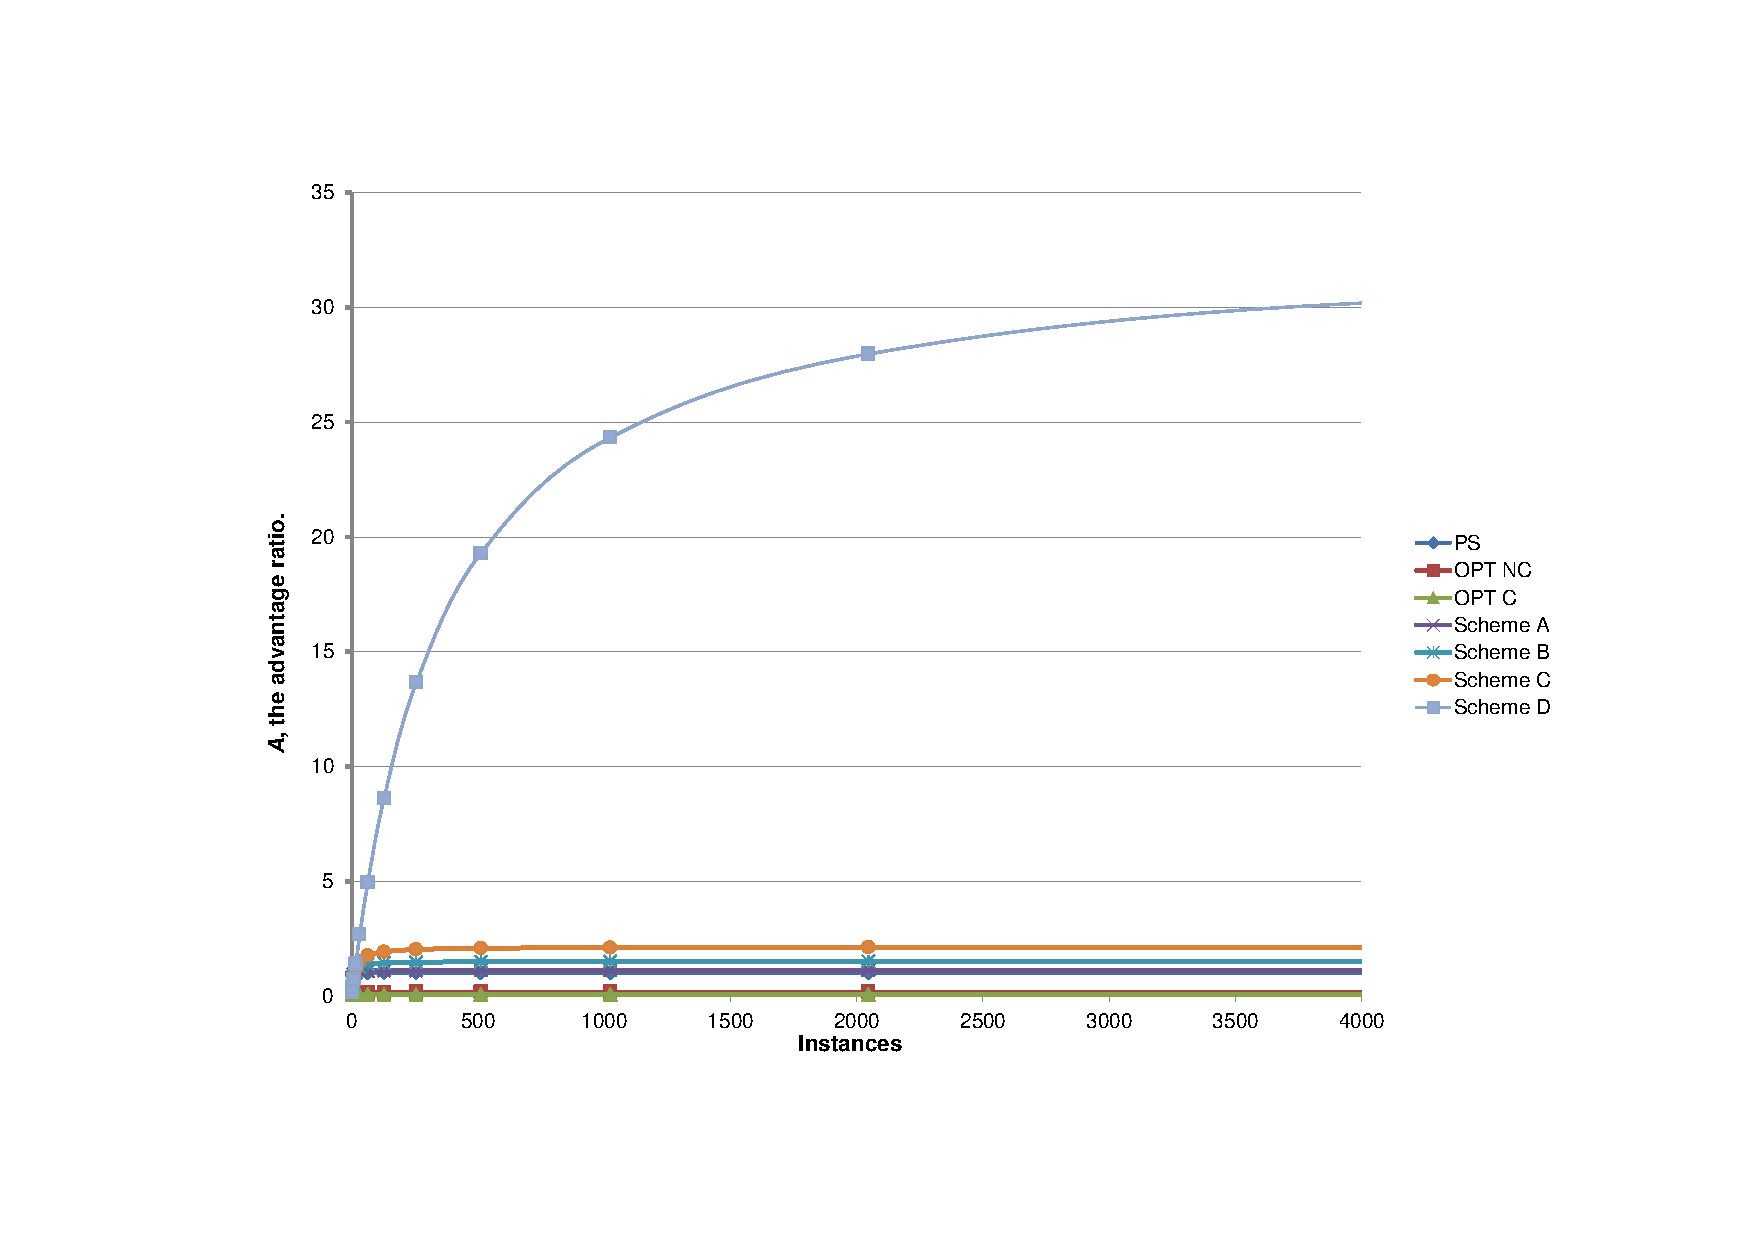
\includegraphics[scale=0.75, trim=5cm 3cm 0cm 3cm]{cups-3.pdf} \label{cups3}} 
  \caption[For \texttt{cups}, $A$ as a function of $N$ (moderately conservative $\vec K$)]% 
          {For \texttt{cups}, $A$ as a function of $N$ (moderately conservative $\vec K$).
          The top graph is a zoomed-in version of the lower graph.}
  \label{cups23}
\end{figure}

For less conservative values of $\vec K$, Figure \ref{cups23} shows that $A$
plateaus at a higher value of $A = 30$ as $N$ gets very large. The maximum
theoretical advantage achievable, $A_{MAX}$ is equal to 194, and we 
are within a factor of $10\times$ that value.

\newpage
\subsection{ntpd}
The Network Time Protocol daemon (\texttt{ntpd}) is a background
service that synchronizes the system time with time servers
using the Network Time Protocol (NTP). \texttt{ntpd}
uses a single configuration file, can operate in both server or client
mode. and can even try to correct for clock skew using a drift file
in the absence of an accessible time server.

\begin{figure}[h]
  \center
  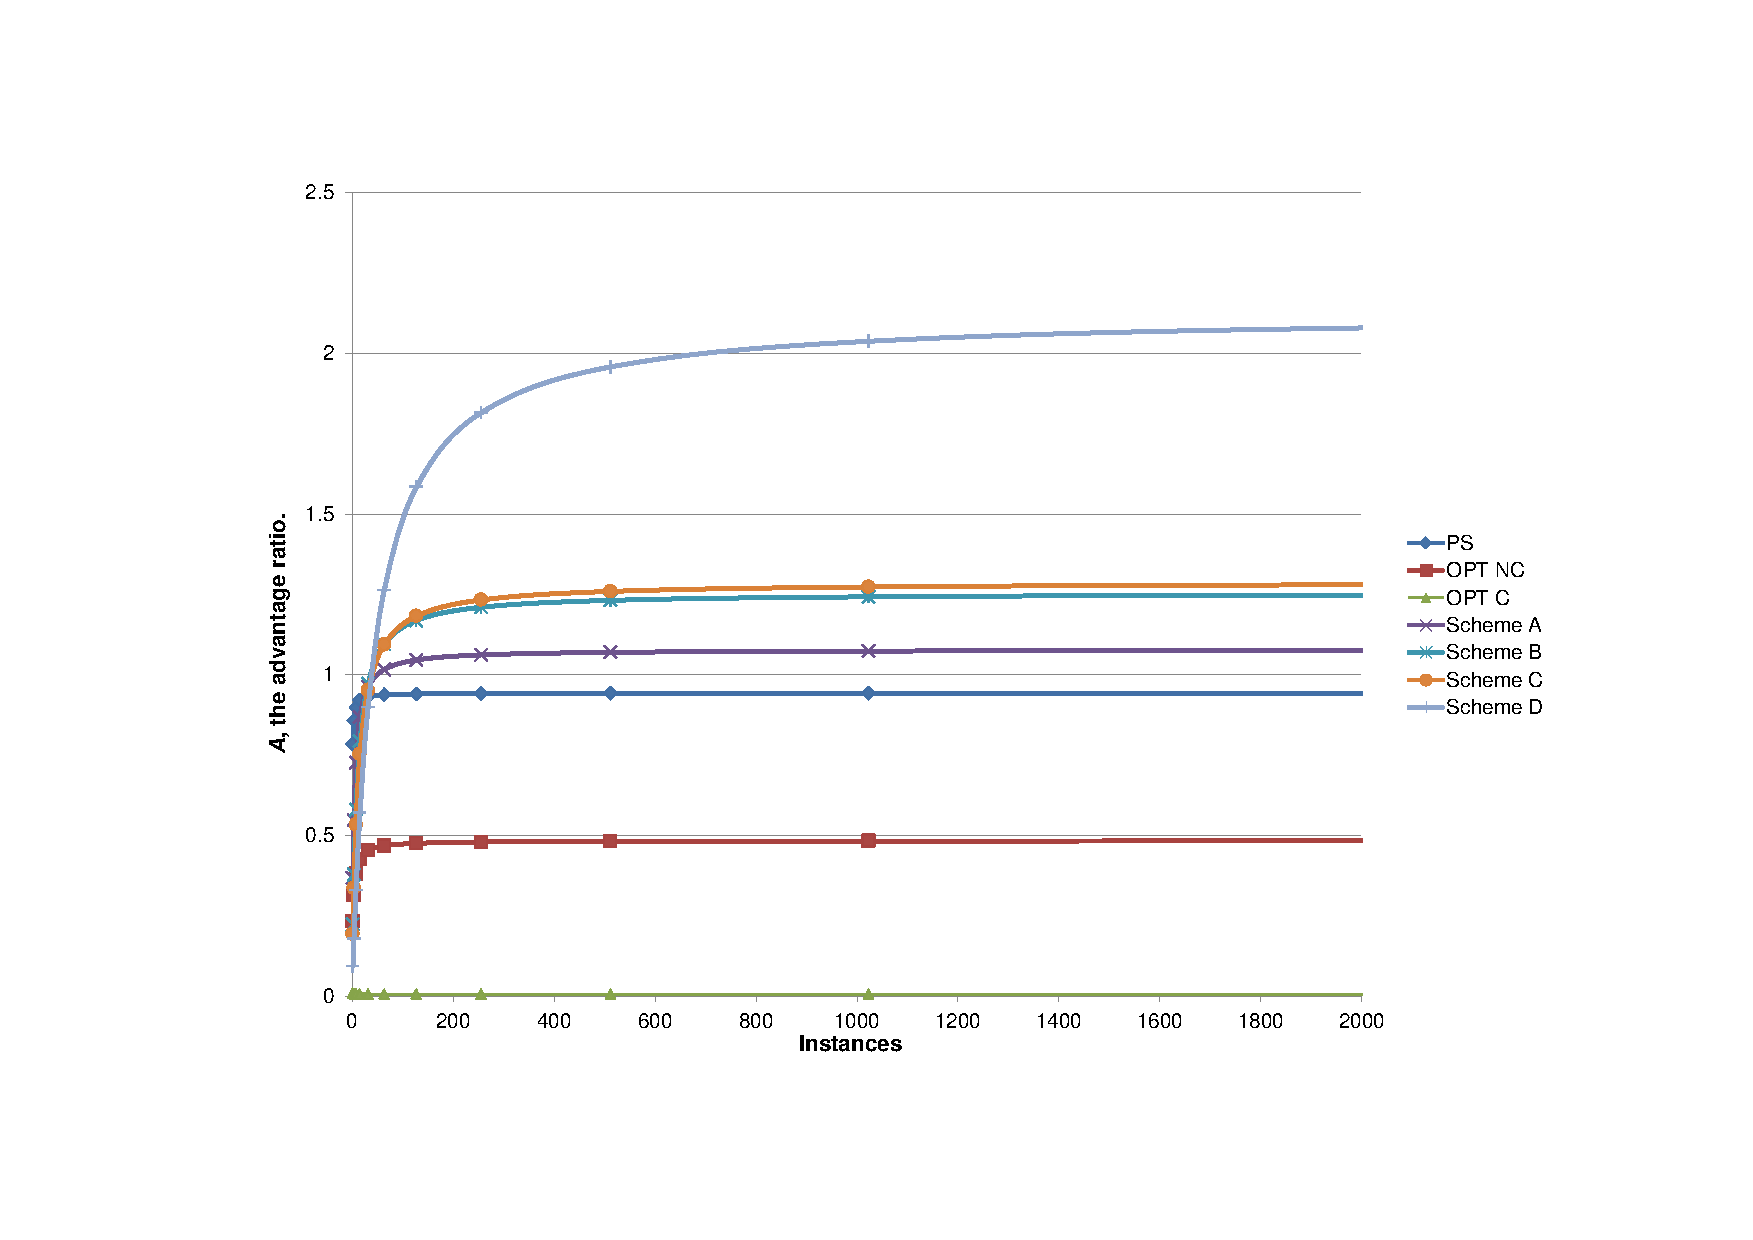
\includegraphics[scale=0.80, trim=5cm 3cm 0cm 3cm]{ntp-1.pdf}
  \caption[For \texttt{ntp}, $A$ as a function of $N$ (highly conservative $\vec K$)]% ]%
          {
            For \texttt{ntpd}, computing $A$ as a function of $N$ (highly conservative $\vec K$).\newline
            \texttt{PS}, \texttt{OPT NC} and \texttt{OPT C} are lines for precise silhouetting, optimistic 
            silhouetting (excluding control flow) and optimistic silhouetting
            (including control flow) without any improvements; they
            serve as a baseline to measure the success of our techniques
            in our simulations. \texttt{Scheme A}, \texttt{Scheme B}, \texttt{Scheme C} and
            \texttt{Scheme D} represent the improved values of $A$
            achieved through incremental levels of deterministic silhouette execution.
          }
  \label{ntp1}
\end{figure}

\newpage
Figure \ref{ntp1} shows how deterministic silhouette execution affects
$A$ for \texttt{ntpd}. The workload considered was a few
iterations of \texttt{ntpd} after it starts up, to simulate
what happens at boot time. The schemes 
for \texttt{ntpd} are the same as those defined for \texttt{cupsd}
in Section \ref{cups:hard}, except that \texttt{Scheme D} 
monitors \texttt{select} events rather than \texttt{epoll}.

For the conservative values of overhead constants ($\vec K$),
\texttt{Scheme D} yields $A > 2$ for $N < 1000$,
which means that the CPU pressure is halved in our simulation of silhouette execution.
This value of $A$ is not as high for
\texttt{ntpd} as for \texttt{cupsd}
because \texttt{ntpd} has almost twice as many memory 
writes as \texttt{cupsd} for the same number of instructions 
(which, in turn, translates into higher overhead for \texttt{ntpd}).

For less conservative values of ($\vec K$), $A$ plateaus
at a value greater than 10. The maximum theoretical
advantage achievable $A_{MAX} = \frac{I}{F+M} = 72$ for 
\texttt{ntpd}, and our simulated $A$ is within a factor of $10\times$ 
of $A_{MAX}$.

\begin{figure}
  \centering
  \subfloat%[Part 1]
           {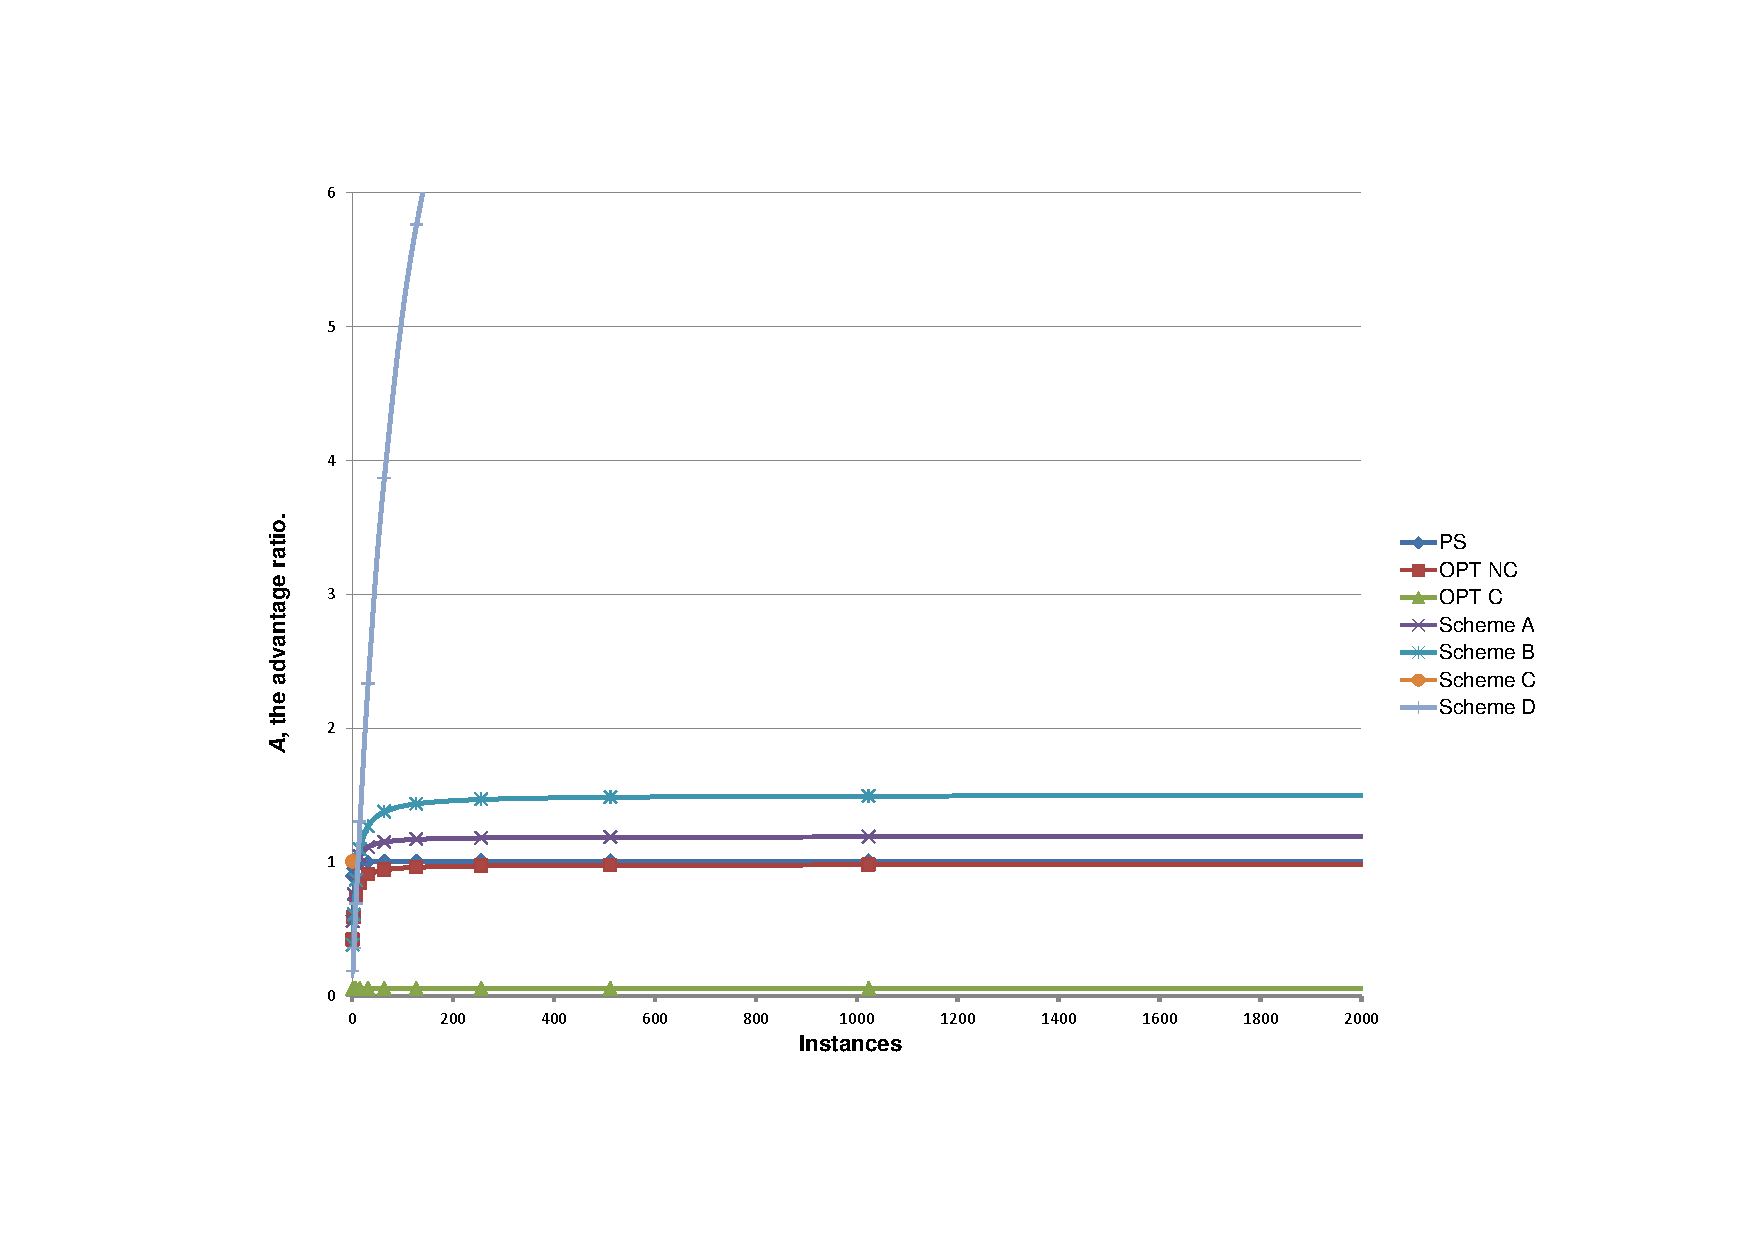
\includegraphics[scale=0.75, trim=5cm 3cm 0cm 4.5cm]{ntp-2.pdf} \label{ntp2}} \\
  \subfloat%[Part 2]
           {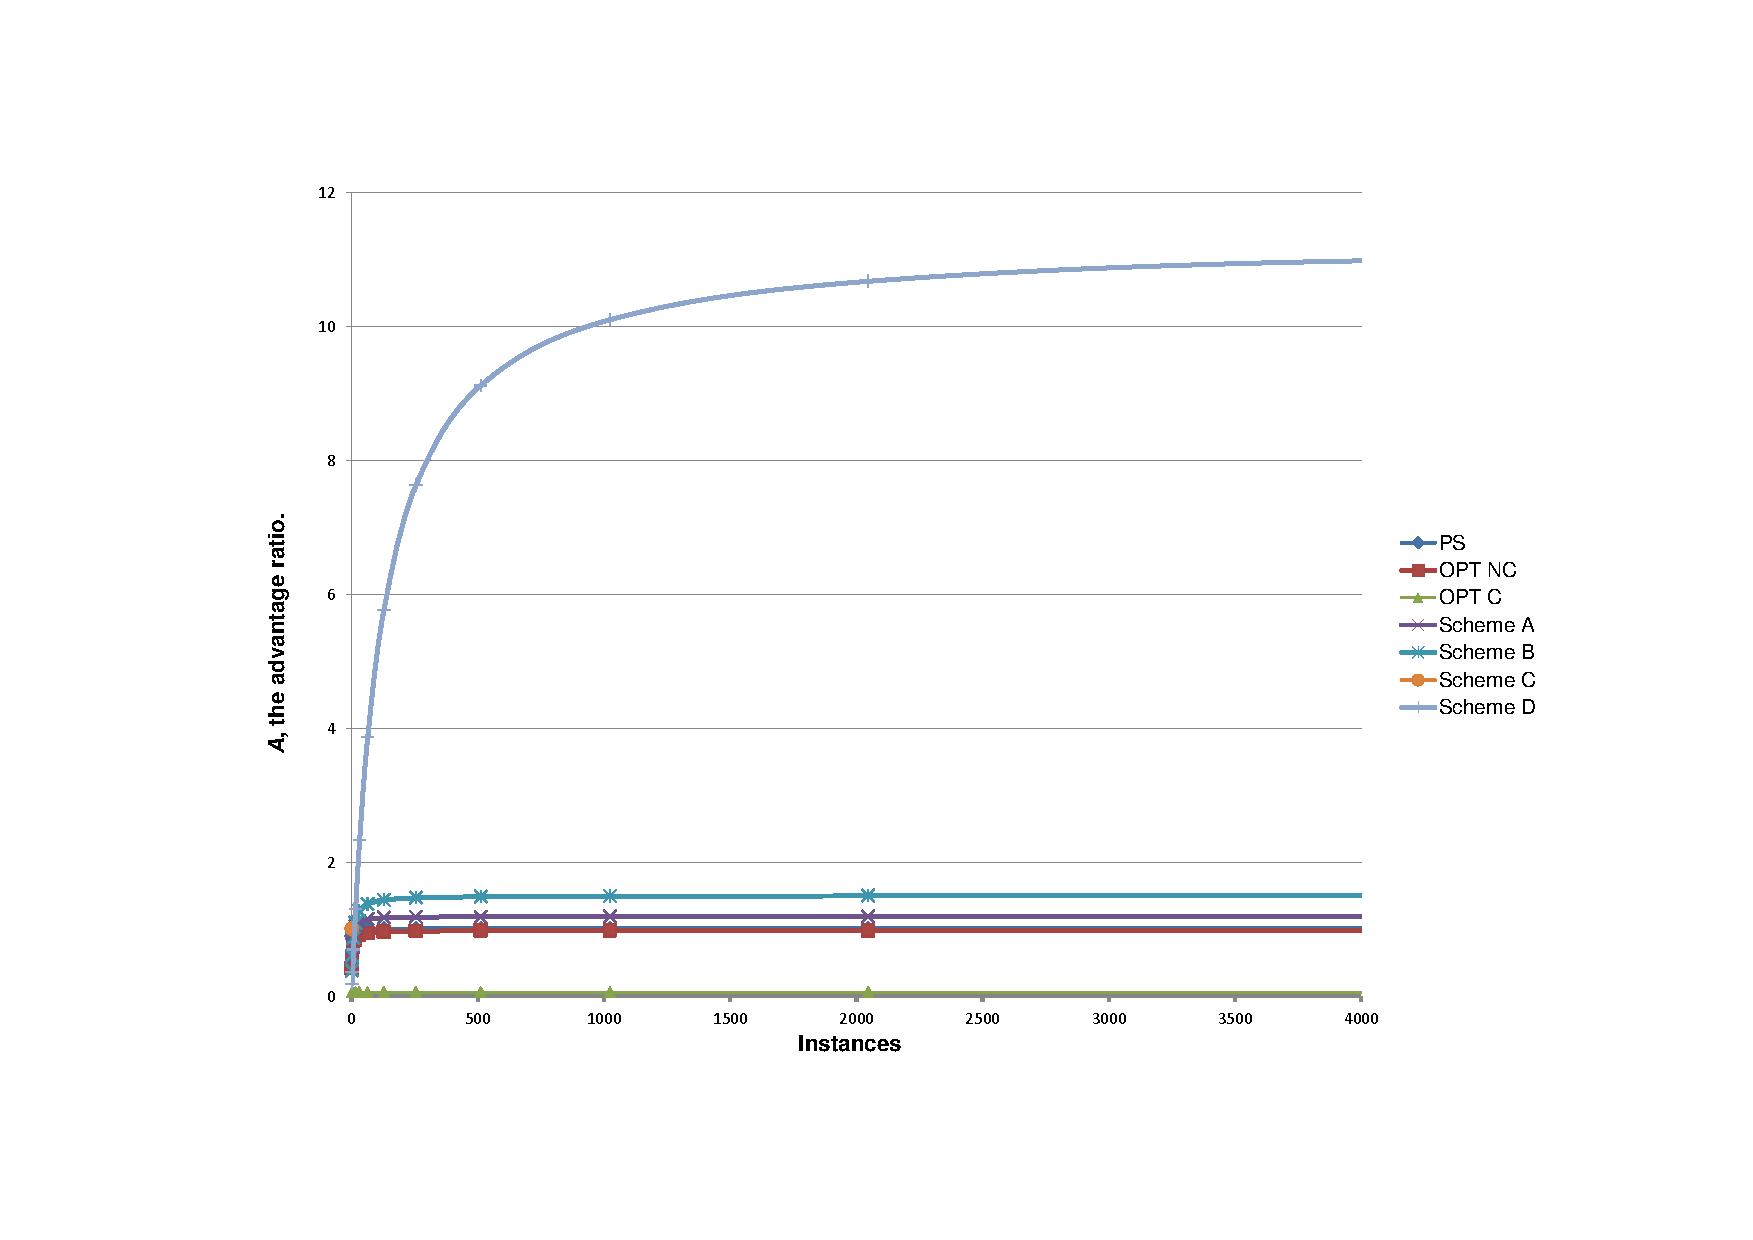
\includegraphics[scale=0.75, trim=5cm 3cm 0cm 3cm]{ntp-3.pdf} \label{ntp3}} 
  \caption[For \texttt{ntpd}, $A$ as a function of $N$ (moderately conservative $\vec K$)]% 
          {For \texttt{ntpd}, $A$ as a function of $N$ (moderately conservative $\vec K$).
          The top graph is a zoomed-in version of the lower graph.}
  \label{ntp23}
\end{figure}

\section{Limitations of Deterministic Execution} \label{ch3:issues}
This section describes some of the drawbacks
of deterministic silhouette execution. \newline

\noindent \textbf{Security} \newline
To achieve deterministic silhouette execution,
we have to disable ASLR. We also have to fix 
canary (\texttt{gs:0x14}) or pointer guard (\texttt{gs:0x18})
values across many different VMs.
Disabling ASLR increases the vulnerability of
applications to external attacks. 
Though canary and pointer guard
values are still dynamically chosen in
our brand of deterministic execution, 
they must agree across all VMs. Thus,
an adversary  who can compromise one VM by
guessing its canary could easily attack the other VMs.
The fact that we can choose different
canary or guard values between different successive boot storms
is some consolation and provides some security. \newline
\newpage
\noindent \textbf{Randomization} \newline
Randomization can be essential for security (e.g. random values
may be used to generate keys or certificates),
performance, and sometimes simply correctness (e.g. 
clients may choose random IDs for themselves).
Making PRNG seeds agree across all VM instances can entail
a compromise on all of these fronts.
In our sample of Linux services, we have not yet discovered any such
issues. Technically,
our approach simulates the extremely unlikely 
-- yet possible -- scenario that all concurrently executing
instances somehow generated the same seeds
from external sources. \newline

\noindent \textbf{Time and Correctness} \newline
Any programs that rely on precise
measurements of time (e.g. through \texttt{rdtsc})
will lose correctness. 
Some Linux services such as \texttt{ntpd} 
do need to measure time accurately in order to synchronize the system clock
Our semantics can cause such services to 
behave incorrectly at start up,
because we may give incorrect values
of time to \texttt{ntpd}.
Thankfully, this is not a huge correctness problem because network 
clock synchronization programs are self-healing and
because we ultimately do provide monotonically
increasing time values. After the booting process is over,
and all VMs branch in execution, \texttt{ntpd} will synchronize
the current time correctly. \newline

\newpage
\section{Summary}
In this chapter, we introduced the general notion of {\em Silhouette Execution},
which is our own design innovation. To study whether silhouette execution
can be effective in solving the boot storm problem, we outlined some design
sketches for silhouette execution in user-space and evaluated their
effectiveness on a few Linux services via simulation and modeling. Preliminary
analysis of silhouette execution was discouraging and showed
an average CPU load {\em increase} in our simulations. We proposed
strategies to control the nondeterminism in Linux services
(e.g. I/O alignment, memory-write compression and process ID virtualization). Through our
simulations in user-space, we found that silhouette execution can reduce CPU
pressure by a factor of $19\times$ on average for $N = 1000$ program instances.



%\appendix
%\chapter{Tables}

\begin{table}
\caption{Armadillos}
\label{arm:table}
\begin{center}
\begin{tabular}{||l|l||}\hline
Armadillos & are \\\hline
our	   & friends \\\hline
\end{tabular}
\end{center}
\end{table}

\clearpage
\newpage

%\chapter{Figures}

\vspace*{-3in}

\begin{figure}
\vspace{2.4in}
\caption{Armadillo slaying lawyer.}
\label{arm:fig1}
\end{figure}
\clearpage
\newpage

\begin{figure}
\vspace{2.4in}
\caption{Armadillo eradicating national debt.}
\label{arm:fig2}
\end{figure}
\clearpage
\newpage

%% This defines the bibliography file (main.bib) and the bibliography style.
%% If you want to create a bibliography file by hand, change the contents of
%% this file to a `thebibliography' environment.  For more information 
%% see section 4.3 of the LaTeX manual.
\begin{singlespace}
\bibliography{main}
\bibliographystyle{plain}
\end{singlespace}

\end{document}

